\documentclass[10pt,twocolumn,letterpaper]{article}

\usepackage{iccv}
\usepackage{times}
\usepackage{epsfig}
\usepackage{graphicx}
\usepackage{color}
\usepackage{caption}
\usepackage{amsmath}
\usepackage{amssymb}
\usepackage{bm}
\usepackage{booktabs}
\usepackage{lib}
\usepackage{algorithm}
\usepackage{algpseudocode}

\algnewcommand{\Initialize}[1]{%
  \State \textbf{Initialize:}
  \Statex \parbox[t]{\linewidth}{\raggedright #1}
}

\usepackage[pagebackref=true,breaklinks=true,letterpaper=true,colorlinks,bookmarks=false]{hyperref}

\iccvfinalcopy % *** Uncomment this line for the final submission

\def\iccvPaperID{1772} % *** Enter the ICCV Paper ID here
\def\httilde{\mbox{\tt\raisebox{-.5ex}{\symbol{126}}}}

% Pages are numbered in submission mode, and unnumbered in camera-ready
\ificcvfinal\pagestyle{empty}\fi
\begin{document}

%%%%%%%%% TITLE
\title{Amodal Completion and Size Constancy in Natural Scenes}
%\title{Object Size from a Single Image}

\author{Abhishek Kar, Shubham Tulsiani, Jo\~{a}o Carreira and Jitendra Malik\\
University of California, Berkeley - Berkeley, CA 94720\\
{\tt\small \{akar,shubhtuls,carreira,malik\}@eecs.berkeley.edu}}

\maketitle
%\thispagestyle{empty}

% Ever since the dawn of computer vision, 3D reconstruction has been a core problem, inspiring early seminal works and leading to numerous real world applications. Much recent progress in the field has been driven by visual recognition systems powered by statistical learning techniques - more recently with convolutional neural networks (CNNs). In this thesis, we attempt to bridge the worlds of geometric 3D reconstruction and learning based recognition by leveraging 3D perception cues from image collections for the task of reconstructing 3D objects.

% In Chapter \ref{chapter:CategoryShapes}, we present a system which is able to learn category-specific deformable 3D models for objects from 2D recognition datasets enabling single view 3D reconstruction for novel instances. In Chapter \ref{chapter:Amodal}, we demonstrate how predicting the amodal extent of objects in images can help us infer their real world heights. Finally, in Chapter \ref{chapter:LSM}, we present Learnt Stereo Machines (LSM), which unify a number of paradigms in 3D object reconstruction - single and multi-view, coarse and dense reconstruction, geometric and semantic reasoning- within an end-to-end learnt framework using convolutional neural networks.

Ever since the dawn of computer vision, 3D reconstruction has been a core problem, inspiring early seminal works and leading to numerous real world applications. Much recent progress in the field however, has been driven by visual recognition systems powered by statistical learning techniques - more recently with deep convolutional neural networks (CNNs). In this thesis, we attempt to bridge the worlds of geometric 3D reconstruction and learning based recognition by learning to leverage various 3D perception cues from image collections for the task of reconstructing 3D objects.

In Chapter \ref{chapter:CategoryShapes}, we present a system that is able to learn intra-category regularities in object shapes by building category-specific deformable 3D models from 2D recognition datasets enabling fully automatic single view 3D reconstruction for novel instances. In Chapter \ref{chapter:Amodal}, we demonstrate how predicting the amodal extent of objects in images and reasoning about their co-occurrences can help us infer their real world heights. Finally, in Chapter \ref{chapter:LSM}, we present Learnt Stereo Machines (LSM), an end-to-end learnt framework using convolutional neural networks, which unifies a number of paradigms in 3D object reconstruction- single and multi-view reconstruction, coarse and dense outputs and geometric and semantic reasoning. We will conclude with several promising future directions for learning based 3D reconstruction.

% Category specific deformable 3D models - Learning shape statistics from annotations in image collections
% Amodal Completion and Size constancy - Learning relative size of objects by observing object co-occurence in image collections
% Learnt Stereo Machines - Unifying single and multi-view resconstruction, geometric and semantic reasoning for 3D reconstruction and coarse and dense prediction by leveraging recent advances in learning based systems (deep neural networks).
Consider the chairs in \figref{fig1_cat}. As humans, not only can we infer at a glance that the image contains three chairs, we also construct a rich internal representation of each of them such as their locations and 3D poses. Moreover, we have a guess of their 3D shapes, even though we might never have seen these particular chairs. We can do this because we do not experience this image {\em tabula rasa}, but in the context of our  ``remembrance of things past".   Previously seen chairs enable us to develop a notion of the 3D shape of chairs, which we can project to the instances in this particular image. We also specialize our representation to these particular instances (e.g. any custom decorations they might have), signalling that both top-down and bottom-up cues influence our percept~\cite{nandakumar2011little}. In this chapter, we incorporate these principles in a computational framewoek for reconstructing objects given a single image. 

The task of reconstructing objects from a single image is a challenging one -- a typical image depicts many objects, each possibly belonging to a different object category; an object category, in turn, comprises instances of varying shapes, textures, size \etc and any particular instance may be viewed from a different viewpoint. Previous approaches to this problem can be broadly grouped into two paradigms. The paradigm of model-based object reconstruction has reflected varying preferences on model representations.  Generalized cylinders~\cite{nevatia1977description} resulted in very compact descriptions for certain classes of shapes, and can be used for category level descriptions, but the fitting problem for general shapes is challenging. Polyhedral models~\cite{gupta2010blocks,xiao2012localizing}, which trace back to the early work of Roberts \cite{roberts1963machine}, and CAD models~\cite{limparsing,satkin20143dnn,Pepik_2015_CVPR_Workshops}, cannot perfectly deform into shapes even slightly different from those in training data, but given a set of point correspondences can be quite effective for determining approximate instance viewpoints. Some recent methods have proposed using similar instances from a collection of CAD models \cite{su2014estimating,huang2015single} for  non-parametric reconstruction but their applications have been restricted to pre-segmented online product images or recovering 3D from 2.5D object scans~\cite{sung2015data}. Here we pursue more expressive basis shape models~\cite{Anguelov:SCAPE2005,blanz1999morphable,zia2013detailed} which establish a balance between the two extremes as they can deform but only along class-specific modes of variation.

\begin{figure}[t]
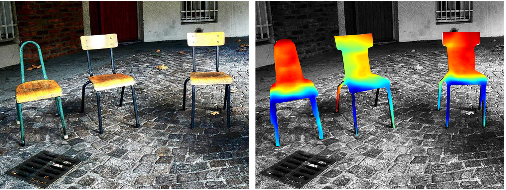
\includegraphics[width = \textwidth]{figures/categoryshapes/teaserChair.pdf}
\caption{Example outputs of our system, given a single image of a scene having chairs, a class that the system was exposed to during training. The coloring on the right image signals object-centric depth (we do not aim for globally consistent depths across multiple objects). Blue means close to the camera, red means far from the camera.}
  \figlabel{fig1_cat}
\end{figure}

The alternate paradigm comprises of approaches that target the problem of object reconstruction in a class or object agnostic manner, either implicitly or explicitly using generic learned 3D shape cues \cite{hoiem2005automatic, saxena2009make3d}, or bottom-up cues and the physics of image formation \cite{Karsch2013,barronPAMI13} building upon the long tradition of Shape-from-X, which traces back to seminal work by Horn \cite{HORNThesis1970}. These methods, while quite general, have not yet been demonstrated for 3D reconstruction -- as opposed to 2.5D -- and typically assume known object segmentation \cite{barronPAMI13}. Some recent approaches have demonstrated the use of supervised learning techniques to implcitly learn generic cues to predict depth maps \cite{eigennips14} and surface normals \cite{eigen2015predicting, wang2015designing} but these have primarily focused on  inferring scene-level information which differs from our goal of perceiving the shape of objects.

In this chapter, we combine both these reconstruction paradigms - we obtain top-down shape information from our model-based reconstruction approach and complement it with bottom-up shape information obtained via an intrinsic image decomposition method.  Crucially, in contrast to previous work (e.g. \cite{barronPAMI13,carvi14,cashman2013dolphins}), we do not require perfect knowledge of object localization and pose as our reconstruction is driven by automatic figure-ground object segmentations and viewpoint estimations.

\begin{figure}[t]
\centering
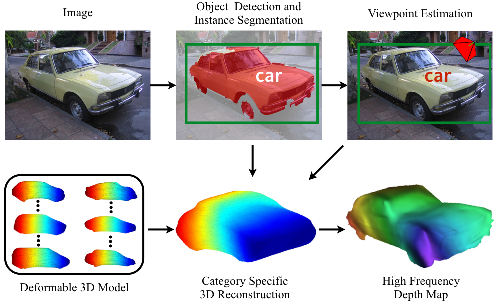
\includegraphics[width = .9\textwidth]{figures/categoryshapes/figTest.pdf}
\caption{Overview of our full reconstruction method. We leverage estimated instance segmentations and predicted viewpoints to generate a full 3D mesh and a high frequency 2.5D depth map for each object in the image.}
\figlabel{figTest}
\end{figure}

The framework we propose to reconstruct the objects present in an image is outlined in \figref{figTest}. As a first step, we leverage the recent progress made by the computer vision community in object detection~\cite{girshick2013rich} and instance segmentation~\cite{BharathECCV2014, BharathCVPR2015} to identify and localize objects in the image. For each object, we also predict a viewpoint in the form of three euler angles. We then use our learned deformable 3D shape models in conjunction with the viewpoint and localization information to produce a ``top-down'' 3D reconstruction for the object guided primarily by category level cues. Finally, we infuse our 3D shape with high frequency local shape cues to obtain our end result - a rich 3D reconstruction of the object. We briefly outline each of the components required for the above proposed framework.

\paragraph{Learning Deformable 3D Models.}
As noted earlier, previously seen objects allow us to develop a notion of 3D shape which informs inference for new instances. We present an algorithm that can build category-specific  deformable shape models from just images with 2D annotations (segmentation masks and a small set of keypoints) present in modern computer vision datasets (e.g. PASCAL VOC~\cite{pascal-voc-2012}). These learnt shape models and deformations allow us to robustly infer shape while capturing intra-class shape variation.

% \paragraph{Learning to Estimate Viewpoint.}
% The first step towards being able to represent objects in 3D is to predict their viewpoint. This intermediate representation provides coarse information about the shape and its inference is a well studied problem in computer vision \cite{huttenlocher1990recognizing, rothganger20063d, gordon2006and, savarese2008view, xiao2008structuring, gu2010discriminative, ozuysal2009pose}.
% We train a Convolutional Neural Network (CNN) ~\cite{neocognitron,LeCun1989} based architecture which can implicitly capture and aggregate local evidence to obtain a viewpoint estimate and demonstrate improvements over the state-of-the-art for this task.

\paragraph{Object Shape Recovery.}
Given an object's category, approximate localization and viewpoint, we obtain a 3D reconstruction for the corresponding object using the learned category-specific deformable shape model. We complement the top-down shape inferred via this inference with a bottom-up module that further refines our shape estimate for a particular instance. This framework allows us to capture the coarse as well as fine level shape details for objects from a single image.

This chapter is organized as follows: in \secref{modelLearning} we describe our model learning pipeline where we estimate camera parameters for all training objects (\secref{nrsfm}) followed by our shape model formulation (\secref{basisshapes}) to learn 3D models. \secref{testing} describes our testing pipeline where we leverage our learnt models alongwith object recognition systems (detection~\cite{girshick2013rich}, segmentation~\cite{BharathCVPR2015}, pose estimation~\cite{ShubhamPose}) to reconstruct novel instances without assuming any annotations. We quantitatively evaluate the various components of our approach in \secref{experiments} and provide sample reconstructions in the wild.

% This journal paper extends our earlier work~\cite{categoryShapesKar15} by providing a detailed exposition of our viewpoint prediction system and its systematic evaluation previously presented in \cite{ShubhamPose}. We also report updated experiments with a slightly modified mesh metric and using improved versions of our pose prediction~\cite{ShubhamPose} and instance segmentation~\cite{BharathCVPR2015} systems.
%\section{Related Work}


Hoiem et al \cite{hoiem2008putting} studied the interaction between object detection and scene layout estimation and showed that reasoning over object sizes within their 3D environment, as opposed to within the image, had a positive impact on detection performance. 

The work Lalonde et al \cite{lalonde2007photo} is close to ours. It estimates average real world sizes of many object categories in the 3D world, from annotated LabelMe data.

This was still in the HOG age  \cite{dalal2005histograms} -- here we leverage the more powerful feature extraction technology we have now to be able to widthstand occlusions and recover metric information.

Building a database of 3d scenes from user annotations \cite{russell2009building}. This is a heavy duty system with quite a broad model, that classifies pairwise relationships into support, attachment, occlusion, etc. On the bright side it assumes every pixel is annotated as belonging in a region. It also does not perform completion and it's not clear  exactly how they recover depth of occluded objects, probably using familiarity, etc.. ?
 
 Other references:
-  Are Cars Just 3D Boxes? – Jointly Estimating the 3D Shape of Multiple Objects. Schindler
-  Towards Scene Understanding with Detailed 3D Object Representations. Schindler
------------------------------------------------------

Psychology:
Do Artists See Their Retinas? Cavanagh

Amodal completion:
Amodal volume completion: 3D visual completion. Fisher


Organization in vision: Essays on Gestalt perception. Kanizsa 1979

%
\documentclass[../thesis.tex]{subfiles}

\begin{document}

%%%%%%%%% TITLE
% \title{Amodal Completion and Size Constancy in Natural Scenes}

% \begin{abstract}
%Towards the goal of enabling vision systems to reason with models of scenes inferred from a single image,  we study the task of enriching recognition system descriptions  with veridical sizes and relative depths of all the objects. 

We consider the problem of enriching current object detection systems with veridical object sizes and relative depth estimates from a single image. There are several technical challenges to this, such as occlusions, lack of calibration data and the scale ambiguity between object size and distance. These have not been addressed in full generality in previous work. Here we propose to tackle these issues by building upon advances in object recognition and using recently created large-scale datasets. We first introduce the task of amodal bounding box completion, which aims to infer the the full extent of the object instances in the image. We then propose a probabilistic framework for learning category-specific object size distributions from available annotations and leverage these in conjunction with amodal completions to infer veridical sizes of objects in novel images. Finally, we introduce a focal length prediction approach that exploits scene recognition to overcome inherent scale ambiguities and demonstrate qualitative results on challenging real-world scenes.
\end{abstract}
\section{Introduction}

% 1. explain constancy and in particular size constancy

Consider \figref{fig1}. Humans can effortlessly perceive two chairs of roughly the same height and tell that one is much closer than the other, though still further away than the person, who is taller than the chairs. Compare this to what a state-of-the-art object detector tells us about the image: that there are two chairs, 120 and 40 pixels tall, and one person with 200 pixels from top to bottom. How can we enable computer vision systems to move beyond this crude 2D representation and allow them to capture richer models of their environments, such as those that humans take for granted?

The 3D world is a lot more structured than it looks like from the retina (or from a camera sensor), where objects jump around with each saccade and grow and shrink as we move closer or farther from them. We do not perceive any of this because our brains have learned priors about how visual inputs correlate with the underlying environment, and this allows us to directly access realistic and rich models of scenes. The priors we use can be categorized as being related to either \textit{geometry} or \textit{familiarity}.

\begin{figure}[t!]
  \centering
  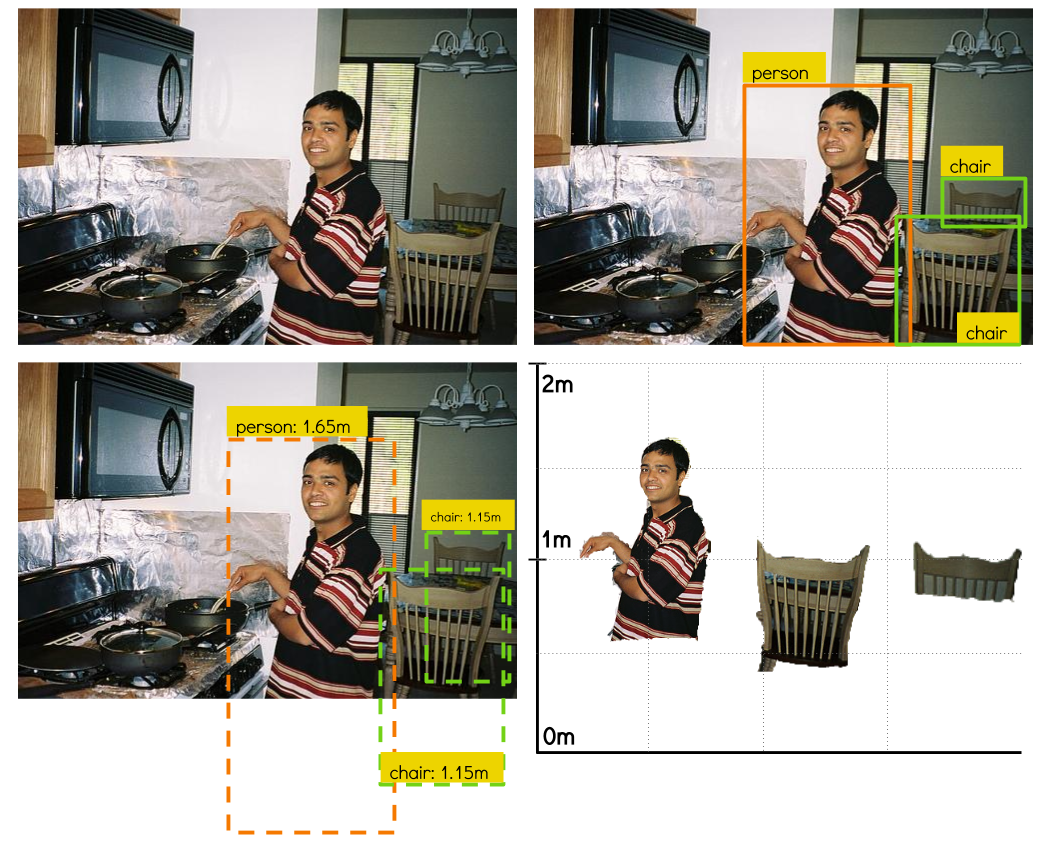
\includegraphics[width=\textwidth]{figures/amodal/Fig_1.png} % COCO_train2014_000000352357.jpg
%  \includegraphics[width=0.22\textwidth]{figures/amodal/coco_occlusions}
  \caption{\figlabel{fig1} Perceiving the veridical size of objects in realistic scenes, from a single image, requires disentangling size and depth, being able to compensate for occlusions and to determine intrinsic camera parameters. We tackle all three of these problems, leveraging recent developments in object recognition and large annotated object and scene datasets.}
\end{figure}

Image projection properties, such as the fact that the distance of an object from the camera dictates apparent size and that parallel lines in the scene vanish in the image, provide useful signal for perceiving structure. Familiarity cues are complementary and impose expectations on individual objects and configurations -- we expect most objects to be supported by another surface and we have the notion of \textit{familiar size} -- similar objects are of similar sizes. In this work, we exploit geometry and familiarity cues and develop a framework to build richer models of the visual input than those given by current computer vision systems, which are still largely confined to the 2D image plane.

The notion that certain geometrical cues can aid perception has been known since the time of Euclid - the points in the image where objects touch the ground together with their perceived heights allows inference of real world object size ratios \cite{burton45}. Familiarity cues, on the other hand must be learned, which can be done using available annotations and building upon rapid recent progress in object recognition, more robustly harnessed to explain novel images. Similar ideas have been proposed by Hoiem \etal~\cite{hoiem2008putting,Hoiem:book} and Gupta \etal ~\cite{gupta2010blocks} who studied the interaction between object detection and scene layout estimation and showed that, by reasoning over object sizes within their 3D environment, as opposed to within the image, one could perform better object detection. Lalonde \etal~\cite{lalonde2007photo} and Russell \etal~\cite{russell2009building} also tackled a problem similar to operationalizing size constancy and inferred object sizes of annotated objects. These works, while sharing similar goals to ours, were limited in their scope as they assumed fully visible instances - object recognition technology at the time being a limiting factor. In this paper, we aim for veridical size estimation in more realistic settings -- where occlusions are the rule rather than the exception. Occlusions present a significant technical challenge as they break down a number of assumptions(\eg in 
\figref{fig1} not modeling occlusions would yield an incorrect estimate of the relative depths of the two chairs shown).

To overcome these challenges, we first introduce amodal completion. This is a very well studied ability of human perception, primarily in the context of amodal edge perception \cite{kanizsa1979organization}, building on theories of \textit{good continuation} \cite{shipley2001fragments}. In the context of objects, amodal completion manifests itself as inference of the complete shape of the object despite visual evidence for only parts of it \cite{breckon2005amodal}.
%Psychology: Do Artists See Their Retinas? Cavanagh
%Amodal completion: Amodal volume completion: 3D visual completion. Fisher
%Organization in vision: Essays on Gestalt perception. Kanizsa 1979
In \secref{amodalCompletion}, we tackle the amodal completion task and frame it as a recognition problem, formalized as  predicting the full extent of object bounding boxes in an image, as opposed to only the visible extent. We build amodal extent predictors based on convolutional neural networks which we train on the challenging PASCAL VOC dataset. In \secref{sizeconstancy}, we propose a formulation that, leveraging amodally completed objects, can disentangle relative object sizes and object distances to the camera. This geometric reasoning allows us only to infer distances for objects up to a scaling ambiguity in each image. To overcome this ambiguity, we show in \secref{sceneFocal} that it is possible to leverage statistical dependencies between scenes and intrinsic camera parameters, and learn to predict focal lengths of scenes from large scale scene datasets. Finally, we present qualitative  results exhibiting veridical size estimation in complex scenes.

%The 3D world is a lot less wild than it looks like from the retina or from a camera sensor. In the retina, due to saccades, objects jump around several times per second. They also grow as we get closer, and get smaller as we move away. The ability to factor out such artifacts of seeing from the true nature of the scenes being seen is called \textit{visual constancy} and makes possible a more seamless interaction of an agent with its environment.


%Computer vision systems are still largely confined to the image plane. For example, in fig. \ref{fig1}, a state-of-the-art object detector localizes three people having heights of 100, 70 and 140 pixels, instead of three people of approximately the same height. Support relationships provide important cues for size constancy by leveraging time-proven Euclidean geometry: the points in the image where objects touch the ground together with their perceived heights allows inference of real world object size ratios \cite{}. Another important cue is familiarity (recognition). As an example, face sizes vary within a narrow range, so their dimensions in the image are informative of nearness to the camera.

%[Say something about size from familiarity (recognition)]

%Both types of cues are affected by occlusions, which translate into depth distortions, but have not yet been considered in prior art \cite{}. In this paper we tackle the size constancy problem in more generality, in realistic settings -- where occlusions are the rule rather than the exception -- by introducing amodal completion. We introduce amodal completion predictors based on convolutional networks which we train on especially engineered datasets having both natural and synthetic occlusion patterns. Additionally, we propose a formulation that, leveraging amodal completion, can disentangle relative class sizes and object distances to the camera from  training data having just ground truth bounding boxes and class labels. Finally, we present qualitative detection results exhibiting size constancy in complex Microsoft COCO scenes. 



%\section{Related Work}


Hoiem et al \cite{hoiem2008putting} studied the interaction between object detection and scene layout estimation and showed that reasoning over object sizes within their 3D environment, as opposed to within the image, had a positive impact on detection performance. 

The work Lalonde et al \cite{lalonde2007photo} is close to ours. It estimates average real world sizes of many object categories in the 3D world, from annotated LabelMe data.

This was still in the HOG age  \cite{dalal2005histograms} -- here we leverage the more powerful feature extraction technology we have now to be able to widthstand occlusions and recover metric information.

Building a database of 3d scenes from user annotations \cite{russell2009building}. This is a heavy duty system with quite a broad model, that classifies pairwise relationships into support, attachment, occlusion, etc. On the bright side it assumes every pixel is annotated as belonging in a region. It also does not perform completion and it's not clear  exactly how they recover depth of occluded objects, probably using familiarity, etc.. ?
 
 Other references:
-  Are Cars Just 3D Boxes? – Jointly Estimating the 3D Shape of Multiple Objects. Schindler
-  Towards Scene Understanding with Detailed 3D Object Representations. Schindler
------------------------------------------------------

Psychology:
Do Artists See Their Retinas? Cavanagh

Amodal completion:
Amodal volume completion: 3D visual completion. Fisher


Organization in vision: Essays on Gestalt perception. Kanizsa 1979

%
\section{Amodal Completion}
\seclabel{amodalCompletion}
\setlength{\epigraphwidth}{.9\textwidth}
\epigraph{``Almost \textit{nothing} is visible in its entirety, yet almost \textit{everything} is perceived as a whole and complete"}{\textit{Stephen Palmer}}

Classic computer vision approaches have traditionally been impoverished by trying to explain just what we see in an image. For years, standard benchmarks have focused on explaining the visible evidence in the image - not the world behind it. For example, the well-studied task of predicting the bounding box around the visible pixels of an object has been the goal of current object detection systems. As humans, not only can we perceive the visible parts of the chair depicted in \figref{fig1}, we can confidently infer the full extent of the actual chair.

This representation of objects, that humans can effortlessly perceive, is significantly richer than what current systems are capable of inferring. We take a step forward towards achieving similar levels of understanding by attacking the task of perceiving the actual extent of the object, which we denote as \textit{amodal completion}. The amodal representation of objects enables us to leverage additional scene information such as support relationships, occlusion orderings etc. For example, given the amodal and visible extents of two neighboring objects in the image, one can figure out if one is occluded by the other. Explicitly modeling amodal representations also allow us to implicitly model occlusions patterns rather than trying to ``explain them away" while detecting objects. As described in \secref{sizeconstancy}, we can use these representations to infer real world object sizes and their relative depths just from images.

The primary focus of object recognition systems \cite{girshick2013rich,felzens_latent_pami10} has been to localize and identify objects, despite occlusions, which are usually handled as noise. Several recently proposed recognition systems do explicitly model occlusion patterns along with detections and provide a mechanism for obtaining amodal extent of the object \cite{ghiasi2014parsing, xiang_cvpr15, zia2014towards}. However, these approaches have been shown to work only on specific categories and rely on available shape models or depth inputs, for learning to reason over occlusions. In contrast, we aim to provide a generic framework that is not limited by these restrictions. Our proposed framework is described below.

\paragraph{Formulation:} Given a candidate visible bounding box, we tackle the task of amodal completion -- the input to our system is some modal bounding box (\eg obtained via a detection system) and we aim to predict the amodal extent for the object. We frame this task as predicting the amodal bounding box, which is defined as  the bounding box of an object in the image plane if the object were completely visible, \ie if inter-object occlusions and truncations were absent. The problem of amodal box prediction can naturally be formulated as a regression task - given a noisy modal bounding box of an object we regress to its amodal bounding box coordinates. The amodal prediction system is implicitly tasked with learning common occlusion/truncation patterns and their effects on visible object size. It can subsequently infer the correct amodal coordinates using the previously learned underlying visual structure corresponding to occlusion patterns. For example, the learner can figure out that chairs are normally vertically occluded by tables and that it should extend the bounding box vertically to predict the full extent of the chair.

Let $b = (x,y,w,h)$ be a candidate visible (or modal) bounding box our amodal prediction system receives ($(x,y)$ are the co-ordinates of the top-left corner and $(w,h)$ are the width and height of the box respectively) and $b^* = (x^*,y^*,w^*,h^*)$ be the amodal bounding box of the corresponding object, our regression targets are $(\frac{x-x^*}{w},\frac{y-y^*}{h},\frac{(x+w)-(x^*+w^*)}{w},\frac{h-h^*}{h})$. Our choice of targets is inspired by the fact that for the $y$ dimension, the height and bottom of the box are the parameters we actually care about (see \secref{sizeconstancy}) whereas along the $x$ dimension the left co-ordinate is not necessarily more important than the right.

\paragraph{Learning:}

We use a Convolutional Neural Network (CNN) \cite{neocognitron,LeCun1989} based framework to predict the co-ordinates of the amodal bounding box. THe hypothesis is that the amodal prediction task can be reliably addressed given just the image corresponding to the visible object region -- seeing the left of a car is sufficient to unambiguously infer the full extent without significantly leveraging context. Based on this observation, we extract from input image $I$, the region corresponding to the detection box $b$ and train the CNN using targets derived as above from the amodal box $b^*$. We impose an $L_2$ penalty on the targets and regress from the extracted CNN image features to the targets. We initialize our model using the AlexNet \cite{krizhevsky2012imagenet} CNN pretrained for Imagenet \cite{imagenet_cvpr09} classification and then finetune the model specific to our task using backpropagation. Training is carried out with jittered instances of the ground truth bounding box to enable generalization from noisy settings such as detection boxes and also serve as data augmentation.

We train two variants of the above network - class-specific and class agnostic. Both these systems comprise of 5 convolutional layers followed by 3 fully-connected layers. The class-specific network has separate outputs in the last layers for different classes and is trained with positive examples from a specific class whereas the class agnostic network has a single set of outputs across all classes. Intuitively, the class-specific network learns to leverage occlusion patterns specific to a particular class (\eg chair occluded by a table) whereas the class agnostic network tries to learn occlusion patterns common across classes. Another argument for a class agnostic approach is that it is unreasonable to expect annotated amodal bounding box data for a large number of categories. A two-stage system, where we first predict the visible bounding box candidates and then regress from them to amodal boxes, enables leveraging these class agnostic systems to generalize to more categories. As we demonstrate in \secref{sizeconstancy}, this class agnostic network can be applied to novel object categories to learn object sizes.

\begin{figure}
  \centering
  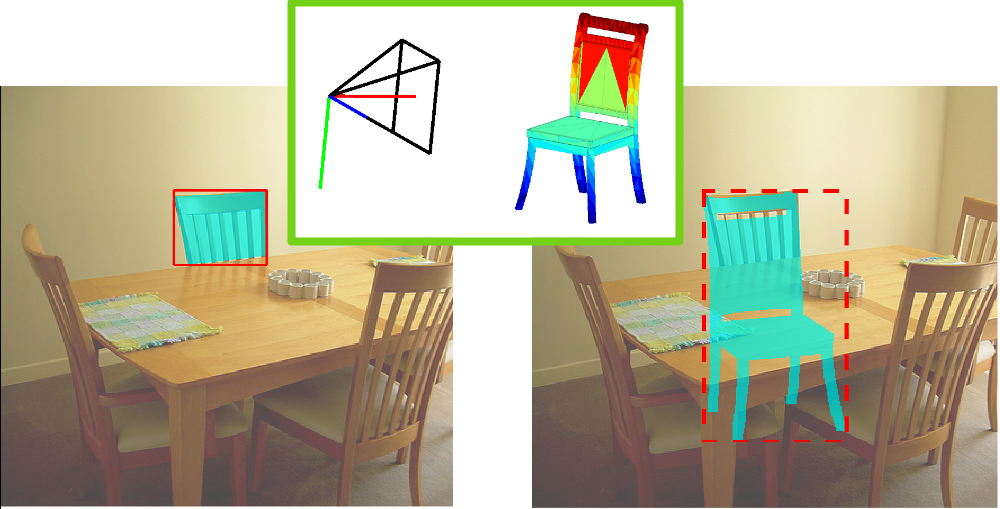
\includegraphics[width=.9\linewidth]{figures/amodal/Amodal.png}
  \caption{\figlabel{amodal} Generating amodal bounding boxes for instances in PASCAL VOC. We use the 3D models aligned to images from the PASCAL 3D+ \cite{pascal3d} and render them with their annotated 3D pose to obtain binary masks. We then use the tightest fitting bounding box around the mask as our ground truth amodal bounding box.}
\end{figure}


%\section{Experiments}
%\seclabel{experiments}
%\subsection{Amodal completion}
\paragraph{Dataset:} For the purpose of amodal bounding box prediction, we need annotations for amodal bounding boxes (unlike visible bounding box annotations present in all standard detection datasets). We use the PASCAL 3D+~\cite{pascal3d} dataset which has approximate 3D models aligned to 12 rigid categories on PASCAL VOC~\cite{pascal-voc-2012} to generate these amodal bounding box annotations. It also contains additional annotations for images from ImageNet \cite{imagenet_cvpr09} for each of these categories (~22k instances in total from ImageNet). For example, it has between 4 different models aligned to ``chair'' and 10 aligned to ``cars''. The different models primarily distinguish between subcategories (but might also be redundant). The 3D models in the dataset are first aligned coarsely to the object instances and then further refined using keypoint annotations. As a consequence, they correctly capture the amodal extent of the object and allow us to obtain amodal ground-truth.  We project the 3D model fitted per instance into the image, extract the binary mask of the projection and fit a tight bounding box around it which we treat as our amodal box (\figref{amodal}). We train our amodal box regressors on the detection training set of PASCAL VOC 2012 (\textit{det-train}) \textit{and} the additional images from ImageNet for these 12 categories which have 3D models aligned in PASCAL 3D+ and test on the detection validation set (\textit{det-val}) from the PASCAL VOC 2012 dataset.

\paragraph{Experiments:} We benchmark our amodal bounding box predictor under two settings - going from ground truth visible bounding boxes to amodal boxes and in a detection setting where we predict amodal bounding boxes from noisy detection boxes. We compare against the baseline of using the modal bounding box itself as the amodal bounding box (\textit{modal bbox}) which is in fact the correct prediction for all untruncated instances. \tableref{gtBboxTable} summarizes our experiments in the former setting where we predict amodal boxes from visible ground truth boxes on various subsets of the dataset and report the mean IoU of our predicted amodal boxes with the ground truth amodal boxes generated from PASCAL 3D+. As expected, we obtain the greatest boost over the baseline for truncated instances. Interestingly, the class agnostic network performs as well the class specific one signaling that occlusion patterns span across classes and one can leverage these similarities to train a generic amodal box regressor. 

To test our amodal box predictor in a noisy setting, we apply it on bounding boxes predicted by the RCNN\cite{girshick2013rich} system from Girshick \etal. We assume a detection be correct if the RCNN bounding box has an IoU $> 0.5$ with the ground truth visible box \textit{and} the predicted amodal bounding box also has an IoU $> 0.5$ with the ground truth amodal box. We calculate the average precision for each class under the above definition of a ``correct'' detection and call it the Amodal $AP$ (or $AP^{am}$). \tableref{detectionTable} presents our $AP^{am}$ results on VOC2012 \textit{det-val}. As we can see again, the class agnostic and class specific systems perform very similarly. The notable improvement is only in a few classes (\eg diningtable and boat) where truncated/occluded instances dominate. Note that we do not rescore the RCNN detections using our amodal predictor and thus our performance is bounded by the detector performance. Moreover, the instances detected correctly by the detector tend to be cleaner ones and thus the baseline (\textit{modal bbox}) of using the detector box output as the amodal box also does reasonably well. Our RCNN detector is based on the VGG16 \cite{simonyan2014very} architecture and has a mean $AP$ of $57.0$ on the 12 rigid categories we consider.

% Latent positives table
\begin{table}[htb!]
\centering
\begin{tabular}{ccccc}
\toprule
& \textbf{all} & \textbf{trun/occ} & \textbf{trunc} & \textbf{occ} \tabularnewline
\midrule

\textbf{modal bbox} & 0.66 & 0.59 & 0.52 & 0.64 \tabularnewline
\textbf{class specific} & 0.68 & 0.62 & 0.57 & 0.65 \tabularnewline
\textbf{class agnostic} & 0.68 & 0.62 & 0.56 & 0.65 \tabularnewline

\bottomrule
\end{tabular}
\caption{Mean IoU of amodal boxes predicted from the visible bounding box on various subsets of the validation set in PASCAL VOC. Here \textit{occ} and \textit{trunc} refer to occluded and truncated instances respectively. The class specific and class agnostic methods refer to our variations of the training the amodal box regressors (see text for details) and modal bbox refers to the baseline of using the visible/modal bounding box itself as the predicted amodal bounding box.}
\tablelabel{gtBboxTable}
\end{table}

% Detection table
\begin{table*}[htb!]
\centering
\resizebox{\linewidth}{!}{
\begin{tabular}{ccccccccccccc|c}
\toprule
& \textbf{aero} & \textbf{bike} & \textbf{boat} & \textbf{bottle} & \textbf{bus} & \textbf{car} & \textbf{chair} & \textbf{table} & \textbf{mbike} & \textbf{sofa} & \textbf{train} & \textbf{tv} & \textbf{mean}\tabularnewline
\midrule

\textbf{modal bbox} & 70.0 & 66.2 & 23.9 & 35.1 & 76.4 & 57.7 & 28.9 & 24.2 & 68.3 & 45.8 & 58.1 & 59.6 & 51.2 \tabularnewline
\textbf{class specific} & 69.5 & 67.2 & \textbf{26.9} & 36.0 & \textbf{77.0} & \textbf{61.4} & \textbf{31.4} & 29.2 & \textbf{69.0} & \textbf{49.4} & \textbf{59.3} & 59.5 & \textbf{53.0} \tabularnewline
\textbf{class agnostic} & \textbf{70.0} & \textbf{67.5} & 26.8 & \textbf{36.3} & 76.8 & 61.3 & 31.1 & \textbf{30.9} & 68.9 & 48.4 & 58.6 & \textbf{59.6} & \textbf{53.0} \tabularnewline
%\midrule
% \textbf{RCNN} & 0.72 & 0.7 & 0.36 & 0.38 & 0.78 & 0.65 & 0.35 & 0.36 & 0.72 & 0.52 & 0.71 & %0.6 & 0.57 \tabularnewline
\bottomrule
\end{tabular}}
\caption{$AP^{am}$ for our amodal bounding box predictors on VOC 2012 \textit{det-val}. $AP^{am}$ is defined as the average precision when a detection is assumed to be correct only when both the modal and amodal bounding boxes have IoU $> 0.5$ with their corresponding ground truths.}
\tablelabel{detectionTable}
\end{table*}

Armed with amodal bounding boxes, we now show how we tackle the problem of inferring real world object sizes from images.

\section{Untangling Size and Depth}
\seclabel{sizeconstancy}
Monocular cues for depth perception have been well-studied in psychology literature and there are two very important cues which emerge that tie object size and depth -  namely familiar size and relative size. Familiar size is governed by the fact that the visual angle subtended by an object decreases with distance from the observer and prior knowledge about the actual size of the object can be leveraged to obtain absolute depth of the object in the scene. Relative size, on the other hand, helps in explaining relative depths and sizes of objects - if we know that two objects are of similar sizes in the real world, the smaller object in the image appears farther. Another simple cue for depth perception arises due to perspective projection - an object further in the world appears higher on the image plane. Leveraging these three cues, we show that one can estimate real world object sizes from just images. In addition to object sizes, we also estimate a coarse viewpoint for each image in the form of the horizon and camera height. 

The main idea behind the algorithm is to exploit pairwise size relationships between instances of different object classes in images. As we will show below, given support points of objects on the ground and some rough estimate of object sizes, one can estimate the camera height and horizon position in the image - and as a result relative object depths. And in turn, given object heights in the image and relative depths, one can figure out the real world object scale ratios. Finally, exploiting these pairwise size evidences across images, we solve for absolute real world sizes (upto a common scale factor or the metric scale factor). Note that we use size and height interchangeably here as our notion of object size here actually refers to the object height.
% Perspective projection figure
\begin{figure}
  \centering
  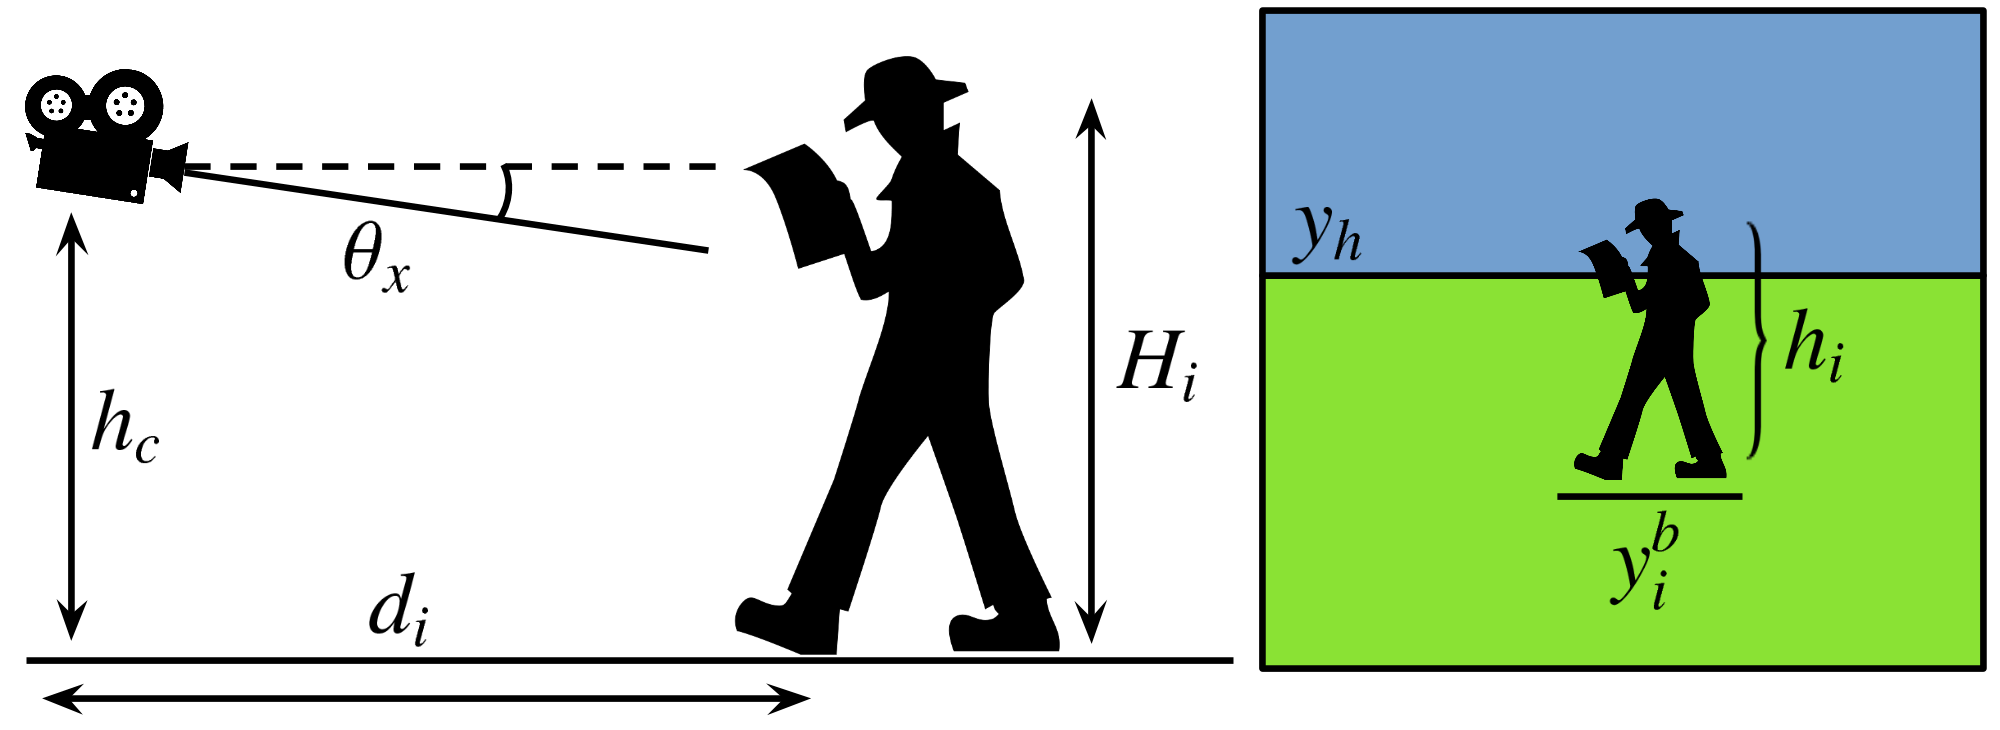
\includegraphics[width=.9\textwidth]{figures/amodal/Perspective.png}
  \caption{\figlabel{perspective} Toy example illustrating our camera model and parameters. Please refer to the text for detailed explanations. }
\end{figure}

\paragraph{Camera Model:} We use a simplified perspective camera model similar to Hoiem \etal~\cite{hoiem2008putting}. Let $f$ be the focal length of the camera, $\theta_x$ the camera tilt angle along the x-axis, $h_c$ the height of the camera, $y_h$ be the horizon position in the image, $y_i^b$ be the ground support point for the $i^{th}$ object in the image and $d_i$ be the distance of the $i^{th}$ object from the camera along the camera axis ($z$ axis). We assume that the images have been corrected for camera roll and all pixel co-ordinates are with respect to the optical center (assumed to be center of the image). \figref{perspective} provides a toy illustration of our model and parameters.

Assuming that the world frame is centered at the camera with its $y$ axis aligned with the ground, the projection of a world point $\mathbf{X} = (X_w,Y_w,Z_w)$ in the image in homogeneous co-ordinates is given by:
\bes
\begin{bmatrix}
x \\
y \\
1
\end{bmatrix} = \frac{1}{Z_w}
\begin{bmatrix}
f & 0 & 0\\
0 & f & 0\\
0 & 0 & 1
\end{bmatrix}
\begin{bmatrix}
1 & 0 & 0 & 0 \\
0 & \cos\theta_x & \sin\theta_x & 0 \\
0 & -\sin\theta_x & \cos\theta_x & 0 \\
\end{bmatrix}
\begin{bmatrix}
X_w \\
Y_w \\
Z_w \\
1
\end{bmatrix}
\ees
For a world point corresponding to the ground contact point of object $i$, given by $(X_w,-h,d_i)$, its corresponding $y$ co-ordinate in the image $y_i^b$ is given by:
$
y_i^b = f\frac{(-h_c/d_i + \tan\theta_x)}{1+(h_c/d_i)\tan\theta_x}
$
Under the assumption of the tilt angle being small ($\tan\theta_x \approx \theta_x$) and height of the camera being not too large compared to object distance ($h\theta_x \ll d_i$), our approximation is 
\be
\eqlabel{groundEq}
y_i^b = -\frac{fh_c}{d_i} + f\theta_x
\ee
Here $f\theta_x$ corresponds to the position of the horizon ($y_h$) in the image. Repeating the above calculation for the topmost point of the object and subtracting from \eqref{groundEq}, we obtain
\be 
\eqlabel{sizeEq}
h_i = \frac{fH_i}{d_i}
\ee
where $h_i$ refers to the height of the object in the image and $H_i$ is the real world height of the object.
Our model makes some simplifying assumptions about the scene namely, objects are assumed to rest on the same horizontal surface (here, the ground) and camera tilt is assumed to be small. We observe that for the purpose of size inference, these assumptions turn out to be reasonable and allow us to estimate heights of objects fairly robustly.

% Algorithm box for size estimation
\begin{algorithm}[h]
\caption{Object Size Estimation}
\begin{algorithmic}
\Initialize{Initial size estimates $\mathbf{H}$ and cluster assignments}
\While {not converged}
\ForAll{images $k \in $ Dataset }
\State $(h_c,y_h) \gets $ SolveLeastSquares($y_b,h,\mathbf{H}$)
\ForAll{pairs $(i,j)$ of objects in $k$}
\State $\frac{H_i}{H_j} \gets \frac{h_i}{h_j}\frac{y_j^b-y_h}{y_i^b-y_h}$\Comment{$(1)$}
\EndFor
\EndFor
\State $\log \mathbf{H} \gets$ least squares with pairwise constraints ($1$)
\State GMM cluster log scales ($\log \mathbf{H}$)
\State Reassign objects to clusters
\EndWhile
\end{algorithmic}
\label{alg:sizeEstimation}
\end{algorithm}

\paragraph{Inferring Object Sizes:} 
The important observation here is that the sizes of objects in an object category are not completely random - they potentially follow a multimodal distribution. For example, different subcategories of boats may represent the different modes of the size distribution. Given some initial sizes and size cluster estimates, our algorithm for size estimation (Algorithm \ref{alg:sizeEstimation}) works by estimating the horizon and camera height per image (by solving a least squares problem using \eqref{groundEq} and \eqref{sizeEq} for all the objects in an image). With the horizon and height estimated per image, we obtain pairwise height ratios $\frac{H_i}{H_j} = \frac{h_i}{h_j}\frac{y_j^b-y_h}{y_i^b-y_h}$ for each pair of objects in an image. We obtain multiple such hypotheses across the dataset which we use to solve a least squares problem for $\log \mathbf{H}$ - the log height for each size cluster. Finally, we cluster the log sizes obtained in the previous step to obtain new size clusters and iterate. Note that $\mathbf{H}$ refers to the vector with heights of various classes and $H_i$ refers to the real world size of the $i^{th}$ object.

This particular model is equivalent to solving a latent variable model where the latent variables are the cluster memberships of the instances, the estimated variables are heights corresponding to the size clusters and the horizon and camera height for each image. The loss function we try to minimize is the mean squared error between the ground contact point predicted by the model and the amodal bounding box. Finally, the log of the object heights are assumed to be a Gaussian mixture. This final assumption ties in elegantly with psychophysics studies which have found that our mental representation of object size (referred to as assumed size~\cite{ittelson1951size,baird1963retinal,epstein1963influence}) is proportional to the logarithm of the real world object size~\cite{konkle2011canonical}.

Our image evidences in the above procedure include the ground support points and heights for all the objects in the image. Note that amodal bounding boxes for objects provide us exactly this information. They account for occlusions and truncations and give us an estimate of the full extent of the object in the image. The above algorithm with occluded/truncated visible bounding boxes would fail miserably and we use our amodal bounding box predictor to first ``complete'' the bounding boxes for us before using our size inference algorithm to infer object heights.

\begin{figure}[htb]
  \centering
  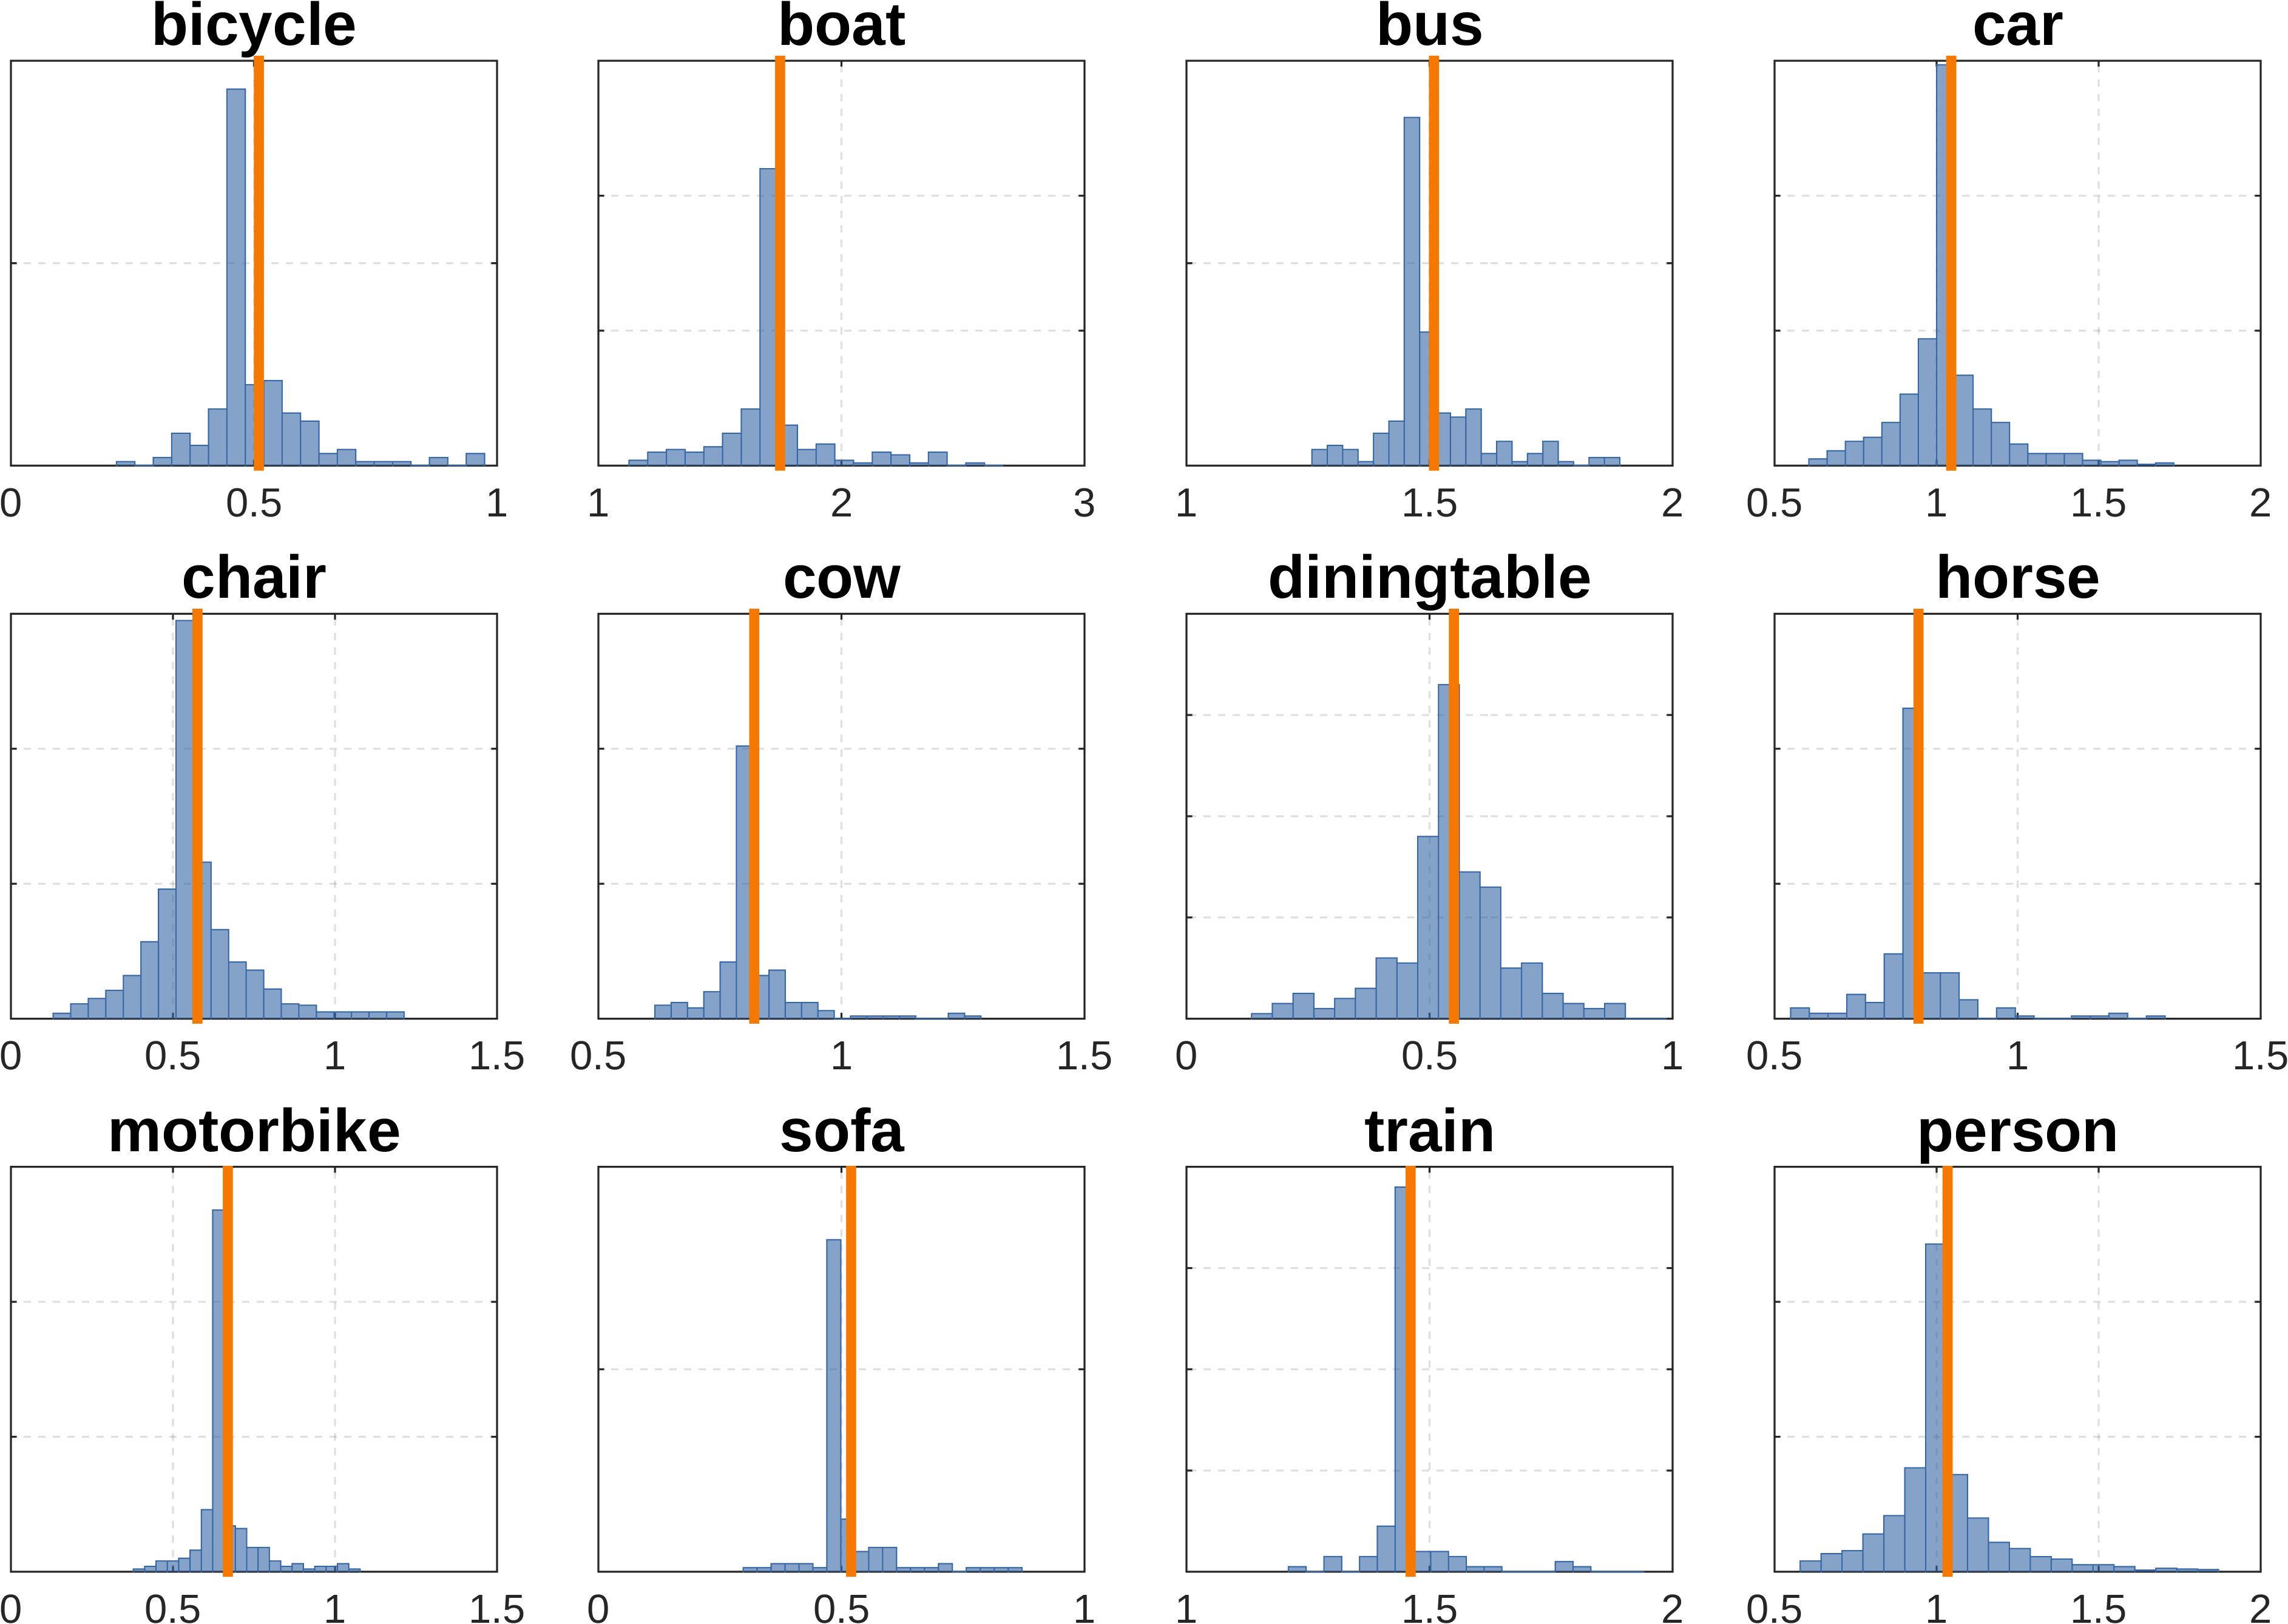
\includegraphics[width=.9\textwidth]{figures/amodal/size_PascalVal_pred.png}
  \caption{\figlabel{pascalSizes} Inferred log size distributions of 12 object categories on PASCAL VOC. We use our class agnostic amodal bounding box predictor to predict amodal boxes for all instances in VOC 2012 \textit{det-val} and use them with our object size estimation system to estimate size distributions for various categories. The plots above show distributions of the log size with the mean size being shown by the orange line.}
\end{figure}

\paragraph{Inferring Object Size Statistics on PASCAL VOC:} We used our size estimation system on PASCAL VOC to estimate size distributions of objects. First, we use our class agnostic amodal bounding box predictor on ground truth visible bounding boxes of all instances on VOC 2012 \textit{det-val} to ``upgrade'' them to amodal boxes. We initialize our system with a rough mean height for each object class obtained from internet sources (Wikipedia, databases of cars etc.) and run our size estimation algorithm on these predicted amodal boxes. \figref{pascalSizes} shows the distributions of log sizes of objects of various categories in PASCAL VOC. Most categories exhibit peaky distributions with classes such as ``boat'' and ``chair'' having longer tails owing to comparatively large intra class variation. Note that we experimented with using multiple size clusters per class for this experiment but the peaky, long tailed nature of these distributions meant that a single Gaussian capturing the log size distributions sufficed. In addition to inferring object sizes, we also infer the horizon position and height of the camera. The median height of the camera across the dataset was 1.4 metres (roughly the height at which people take images) and also exhibited a long tailed distribution (please refer to supplementary for details). Some examples of amodal bounding boxes estimated for all instances from visible bounding boxes and horizons are shown in \figref{resultFig}.



\section{Scenes and Focal Lengths}
\seclabel{sceneFocal}
The focal length of a camera defines its field of view and hence determines how much of a scene is captured in an image taken by the camera. It is an important calibration parameter for obtaining metric, as opposed to projective, measurements from images. It is usually calibrated using multiple images of a known object \cite{zhang2000flexible}, such as a chessboard, or as part of bundle adjustment \cite{triggs2000bundle}, from multiple images of realistic scenes. Well known existing approaches require a minimum set of vanishing lines  \cite{wang1991camera} or exploit Manhattan-world assumptions \cite{caprile1990using}. These techniques are very precise and elegant, but not generally applicable (e.g. beach or forest images, \etc).

We propose instead a learning approach that predicts focal length based on statistical dependencies between scene classes and fields of view. Given the same scene, images taken with large focal lengths will have fewer things in them than those captured with small focal lengths and this provides a cue for determining focal length. However certain scenes also have more things than others. This ambiguity can be resolved by training a predictor with many images of each scene class, taken with different focal lengths. 

Additionally, certain scenes tend to be pictured with preferred focal lengths. As an example, consider a scene class of ``pulpits". If a picture of a pulpit is taken with a short focal length, then the whole church will be visible and that image will not be tagged as a pulpit scene. In order for a pulpit to be dominant in a picture taken with a short focal length camera, then the photographer would have to be unnaturally close to it. 

\paragraph{Data:} We use the Places database \cite{zhou2014learning}, a large dataset that provides a dense sampling of scenes in natural images: it has $205$ scene classes, as diverse as \textit{swimming pool} and \textit{rope bridge}, and $2.5$ million images. We were able to scrape focal length metadata from EXIF tags of approximately $20$k examples, on average 100 per class, and split these into a training set having $15$k and a validation set of $5$k images. 

\paragraph{Learning:} We considered the problem of predicting the ratio of the focal length to the camera sensor width, which when multiplied by the size of the image in pixels gives the desired the focal length in pixels. We clustered the logarithm of this ratio into $10$ bins using k-means and formulated the prediction problem as classification, using a softmax loss. Images in the bin with highest and smallest focal length ratio are shown in \figref{focal_lengths}. We experimented finetuning different popular convolutional networks, including two trained on Imagenet classification -- AlexNet \cite{krizhevsky2012imagenet} and VGG-Deep16 \cite{simonyan2014very} -- and a network trained on the Places scenes -- the PlacesNet \cite{zhou2014learning}.

\begin{figure}[htb!]
  \centering
  \includegraphics[width=0.32\textwidth]{figures/amodal/highest4}
  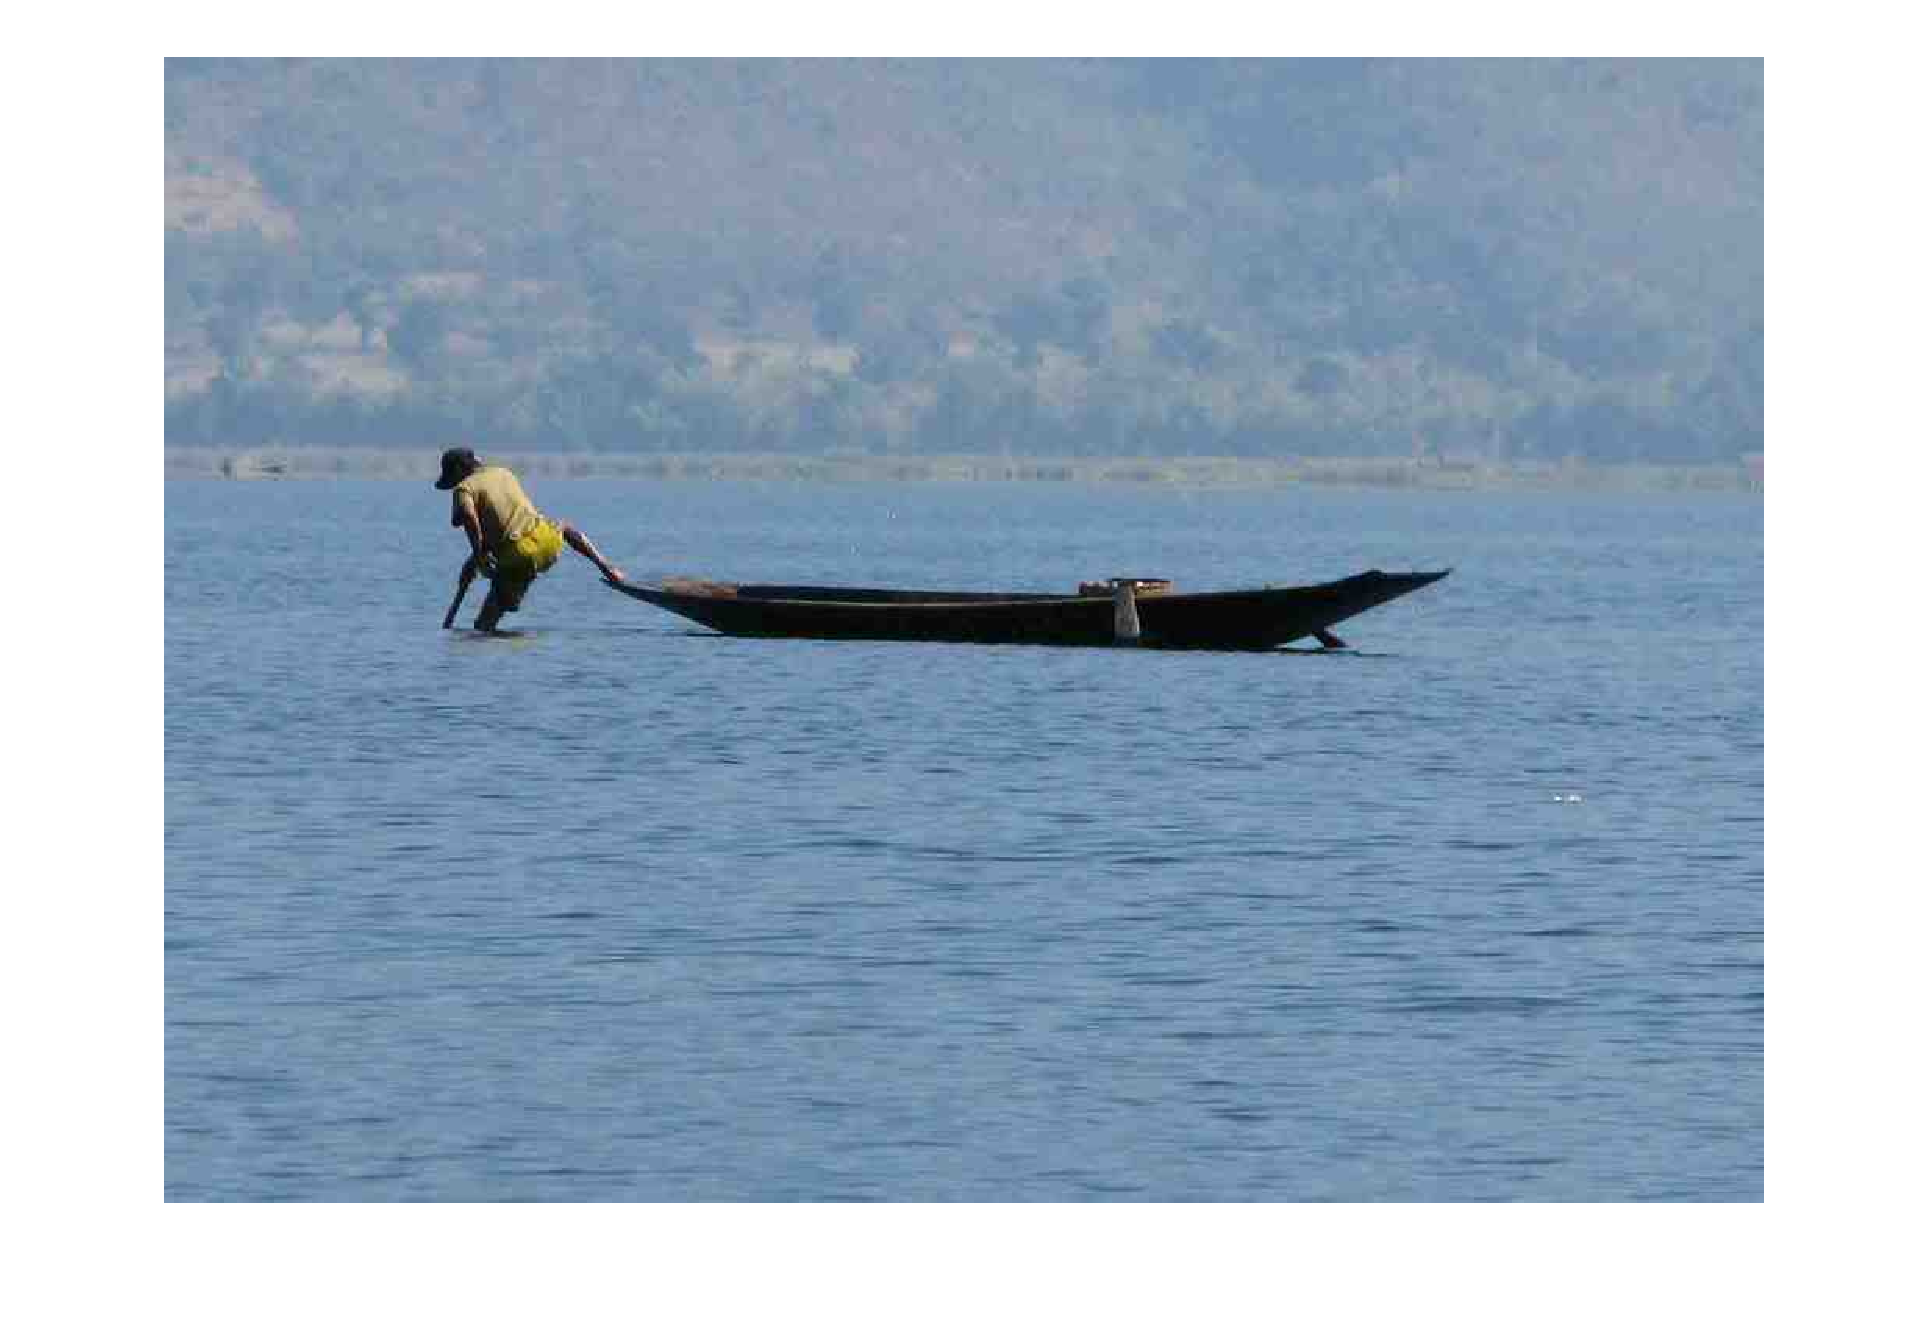
\includegraphics[width=0.32\textwidth]{figures/amodal/highest3}  
  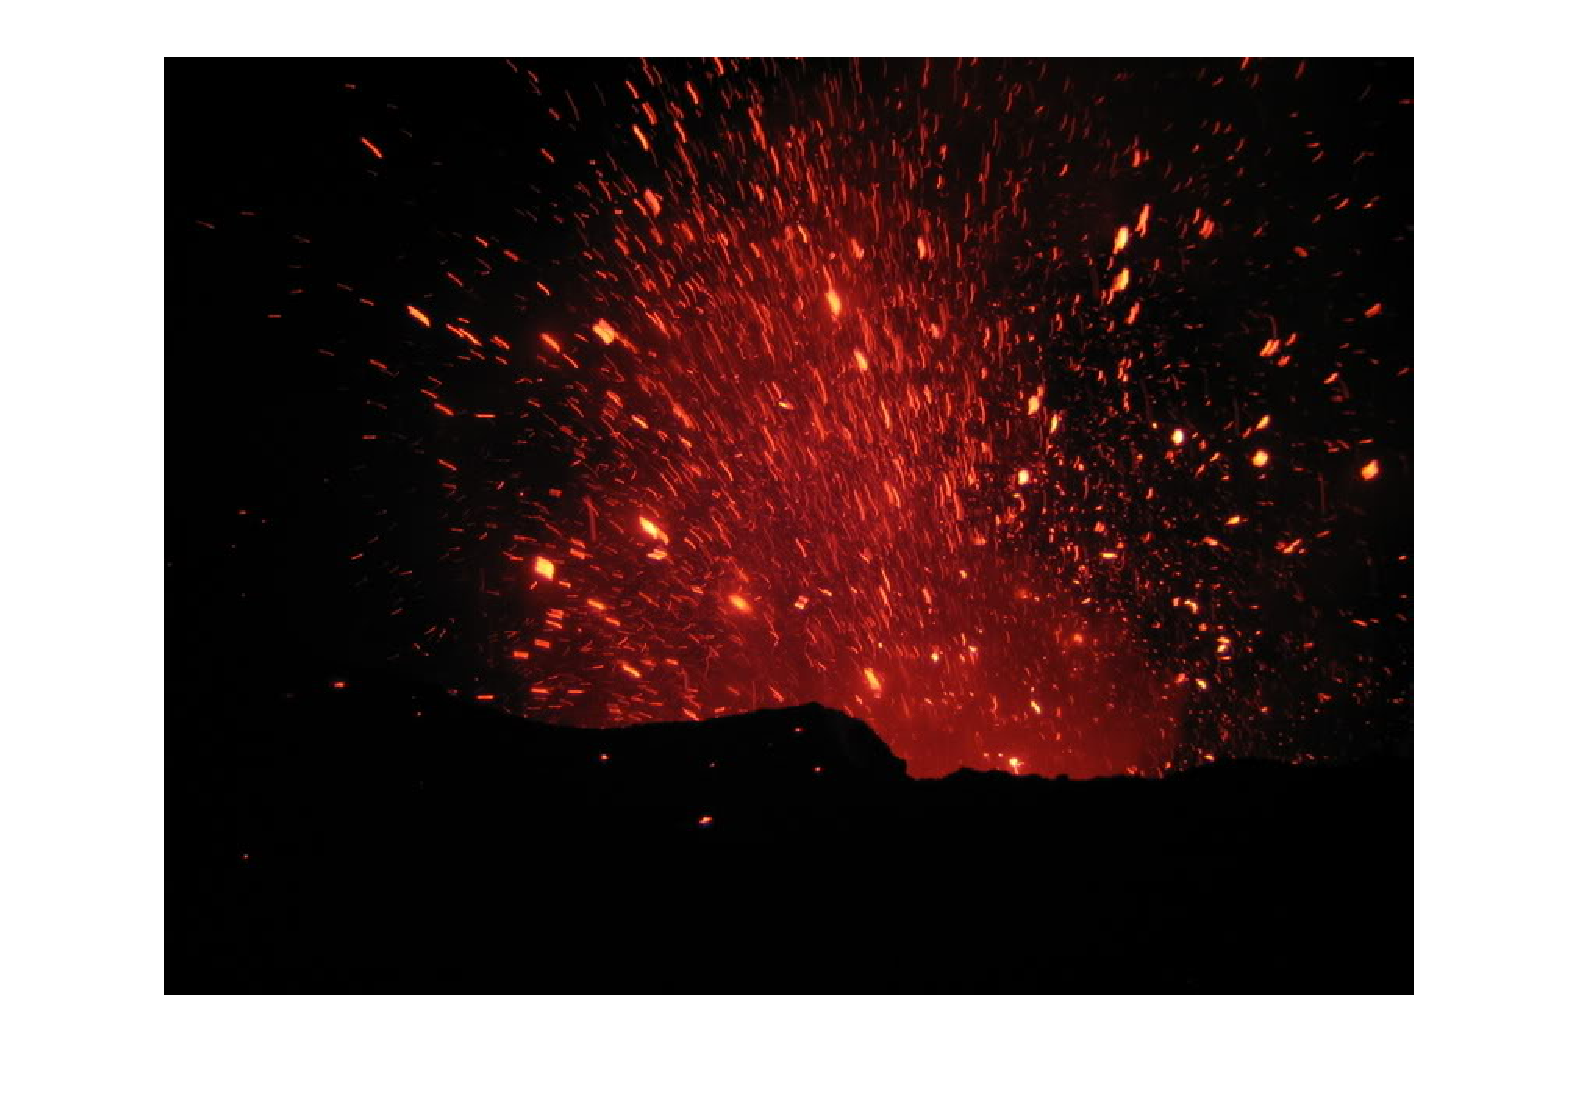
\includegraphics[width=0.32\textwidth]{figures/amodal/highest6}  
  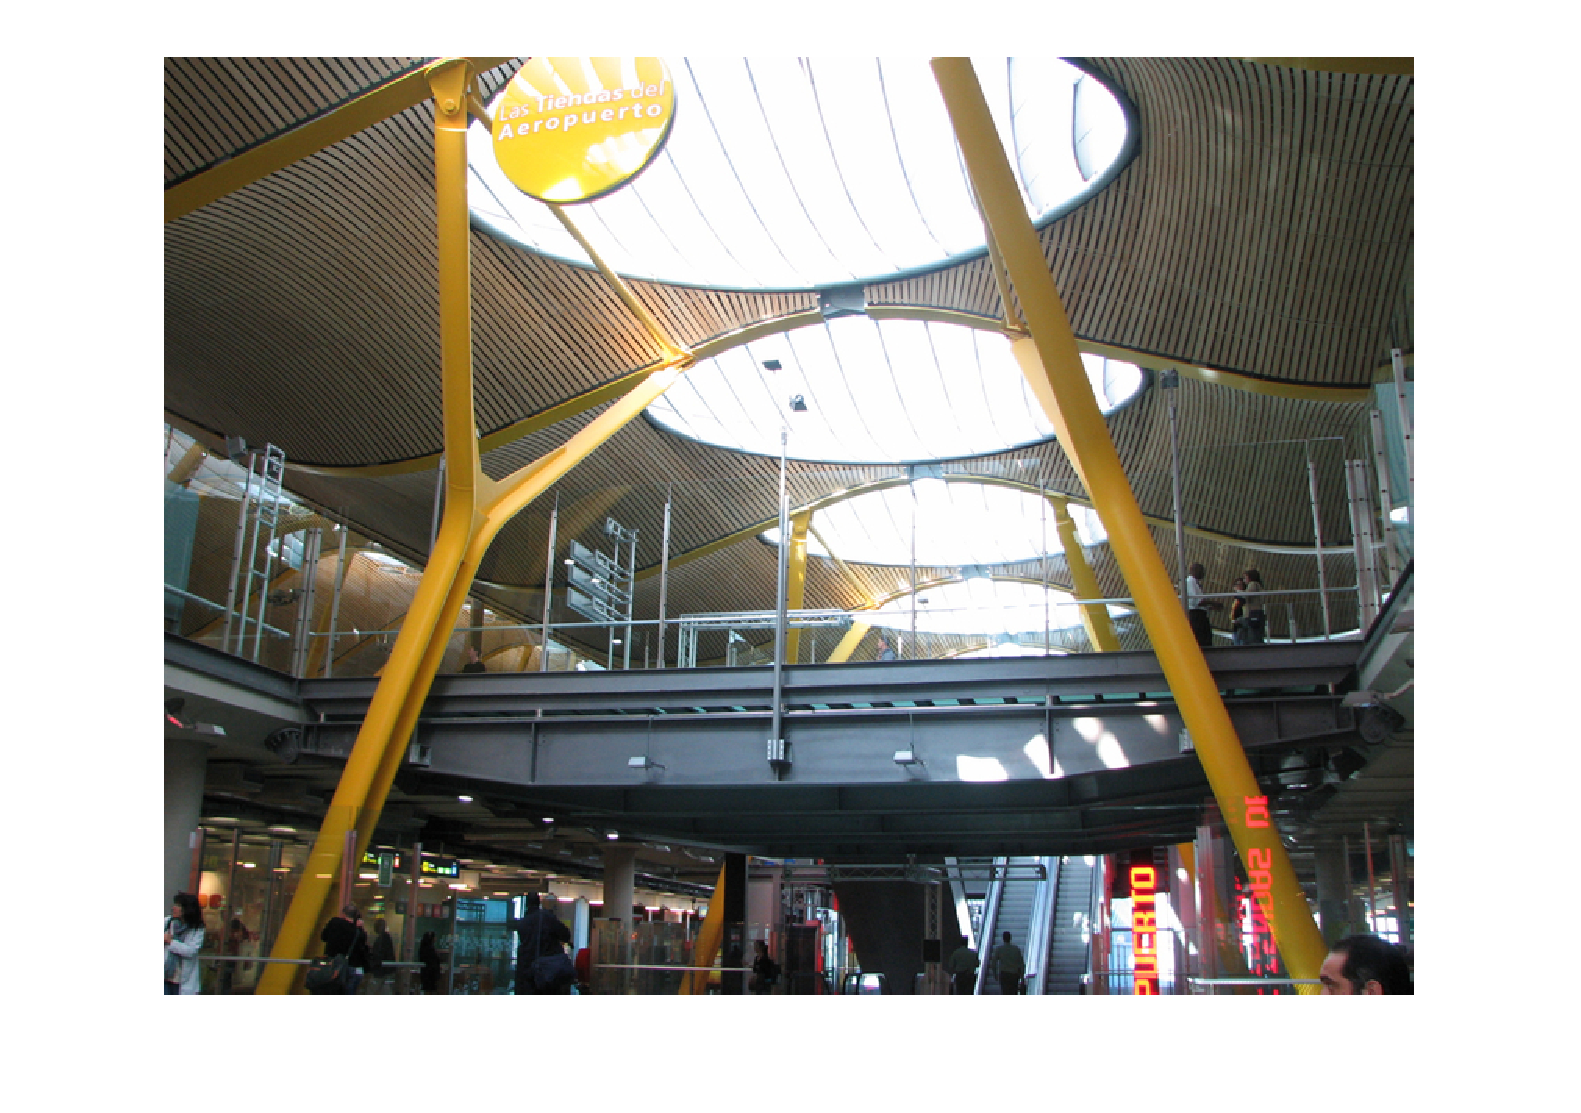
\includegraphics[width=0.32\textwidth]{figures/amodal/lowest1}
  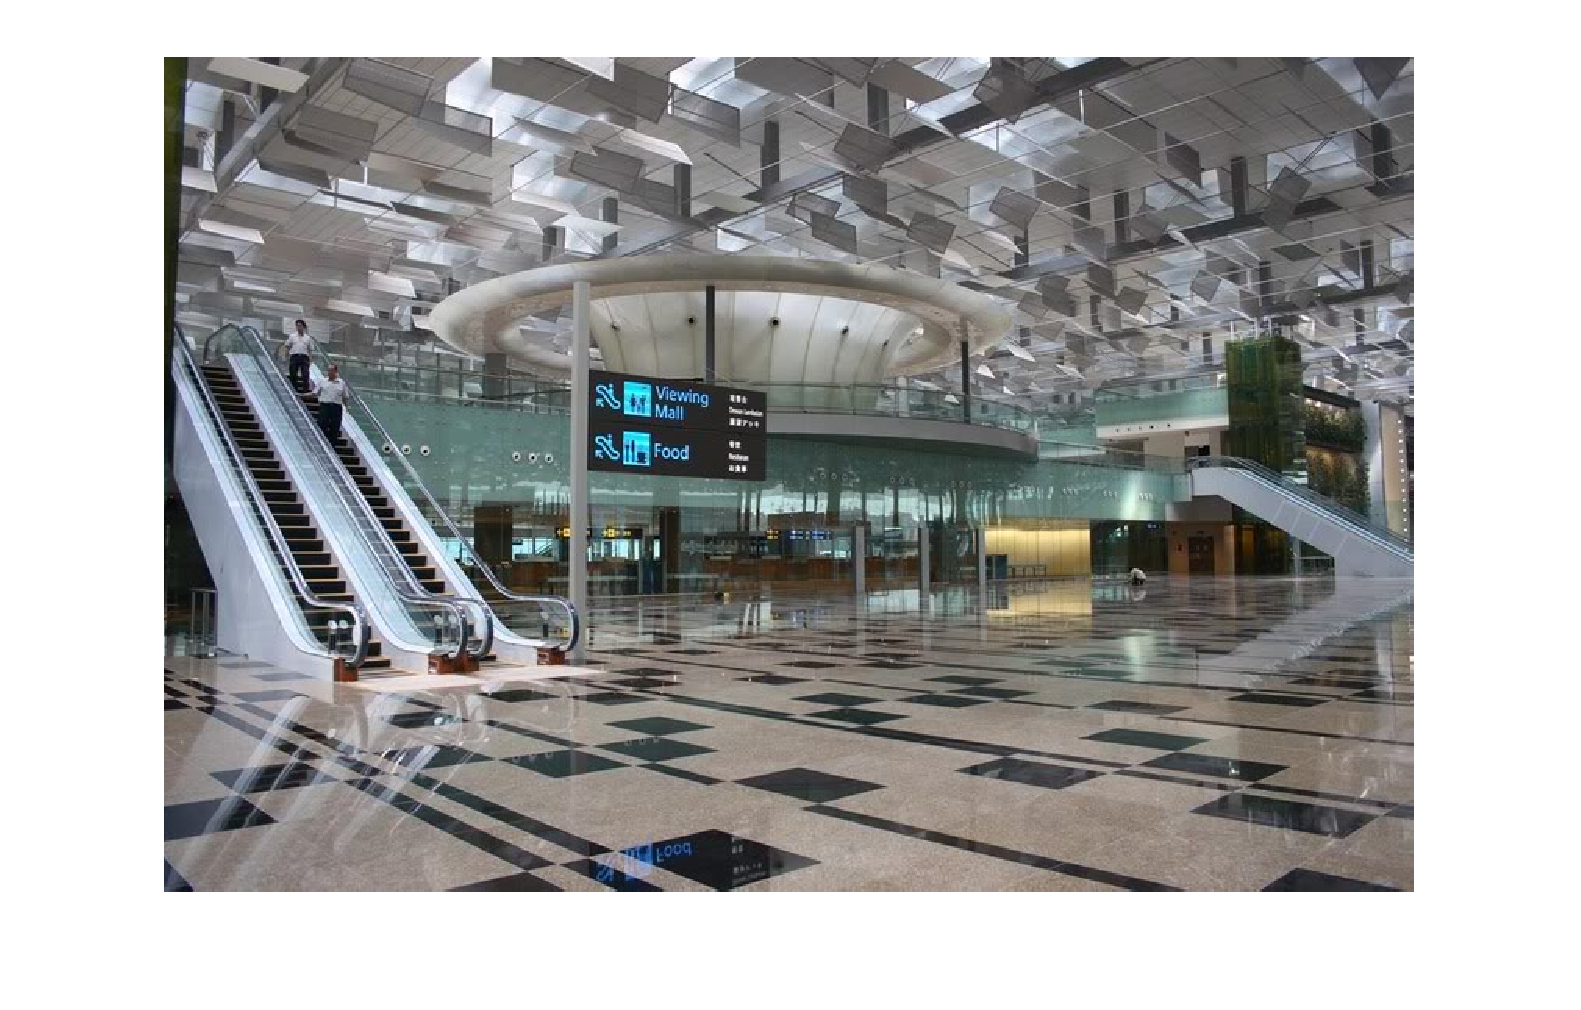
\includegraphics[width=0.32\textwidth]{figures/amodal/lowest3}  
  \includegraphics[width=0.32\textwidth]{figures/amodal/lowest7}
  \caption{\figlabel{focal_lengths} Example images from the Places dataset from clusters with the largest (up) and smallest (down) focal lengths. Note how images with small focal lengths tend to be more cluttered. A pattern we observed is that dangerous or unaccessible scenes, such as those having volcanos, wild animals and boats tend to be captured using very-high focal lengths,  which is rational.}
\end{figure}

\begin{figure}[htb!]
  \centering
  \begin{minipage}{.45\textwidth}
    \centering
    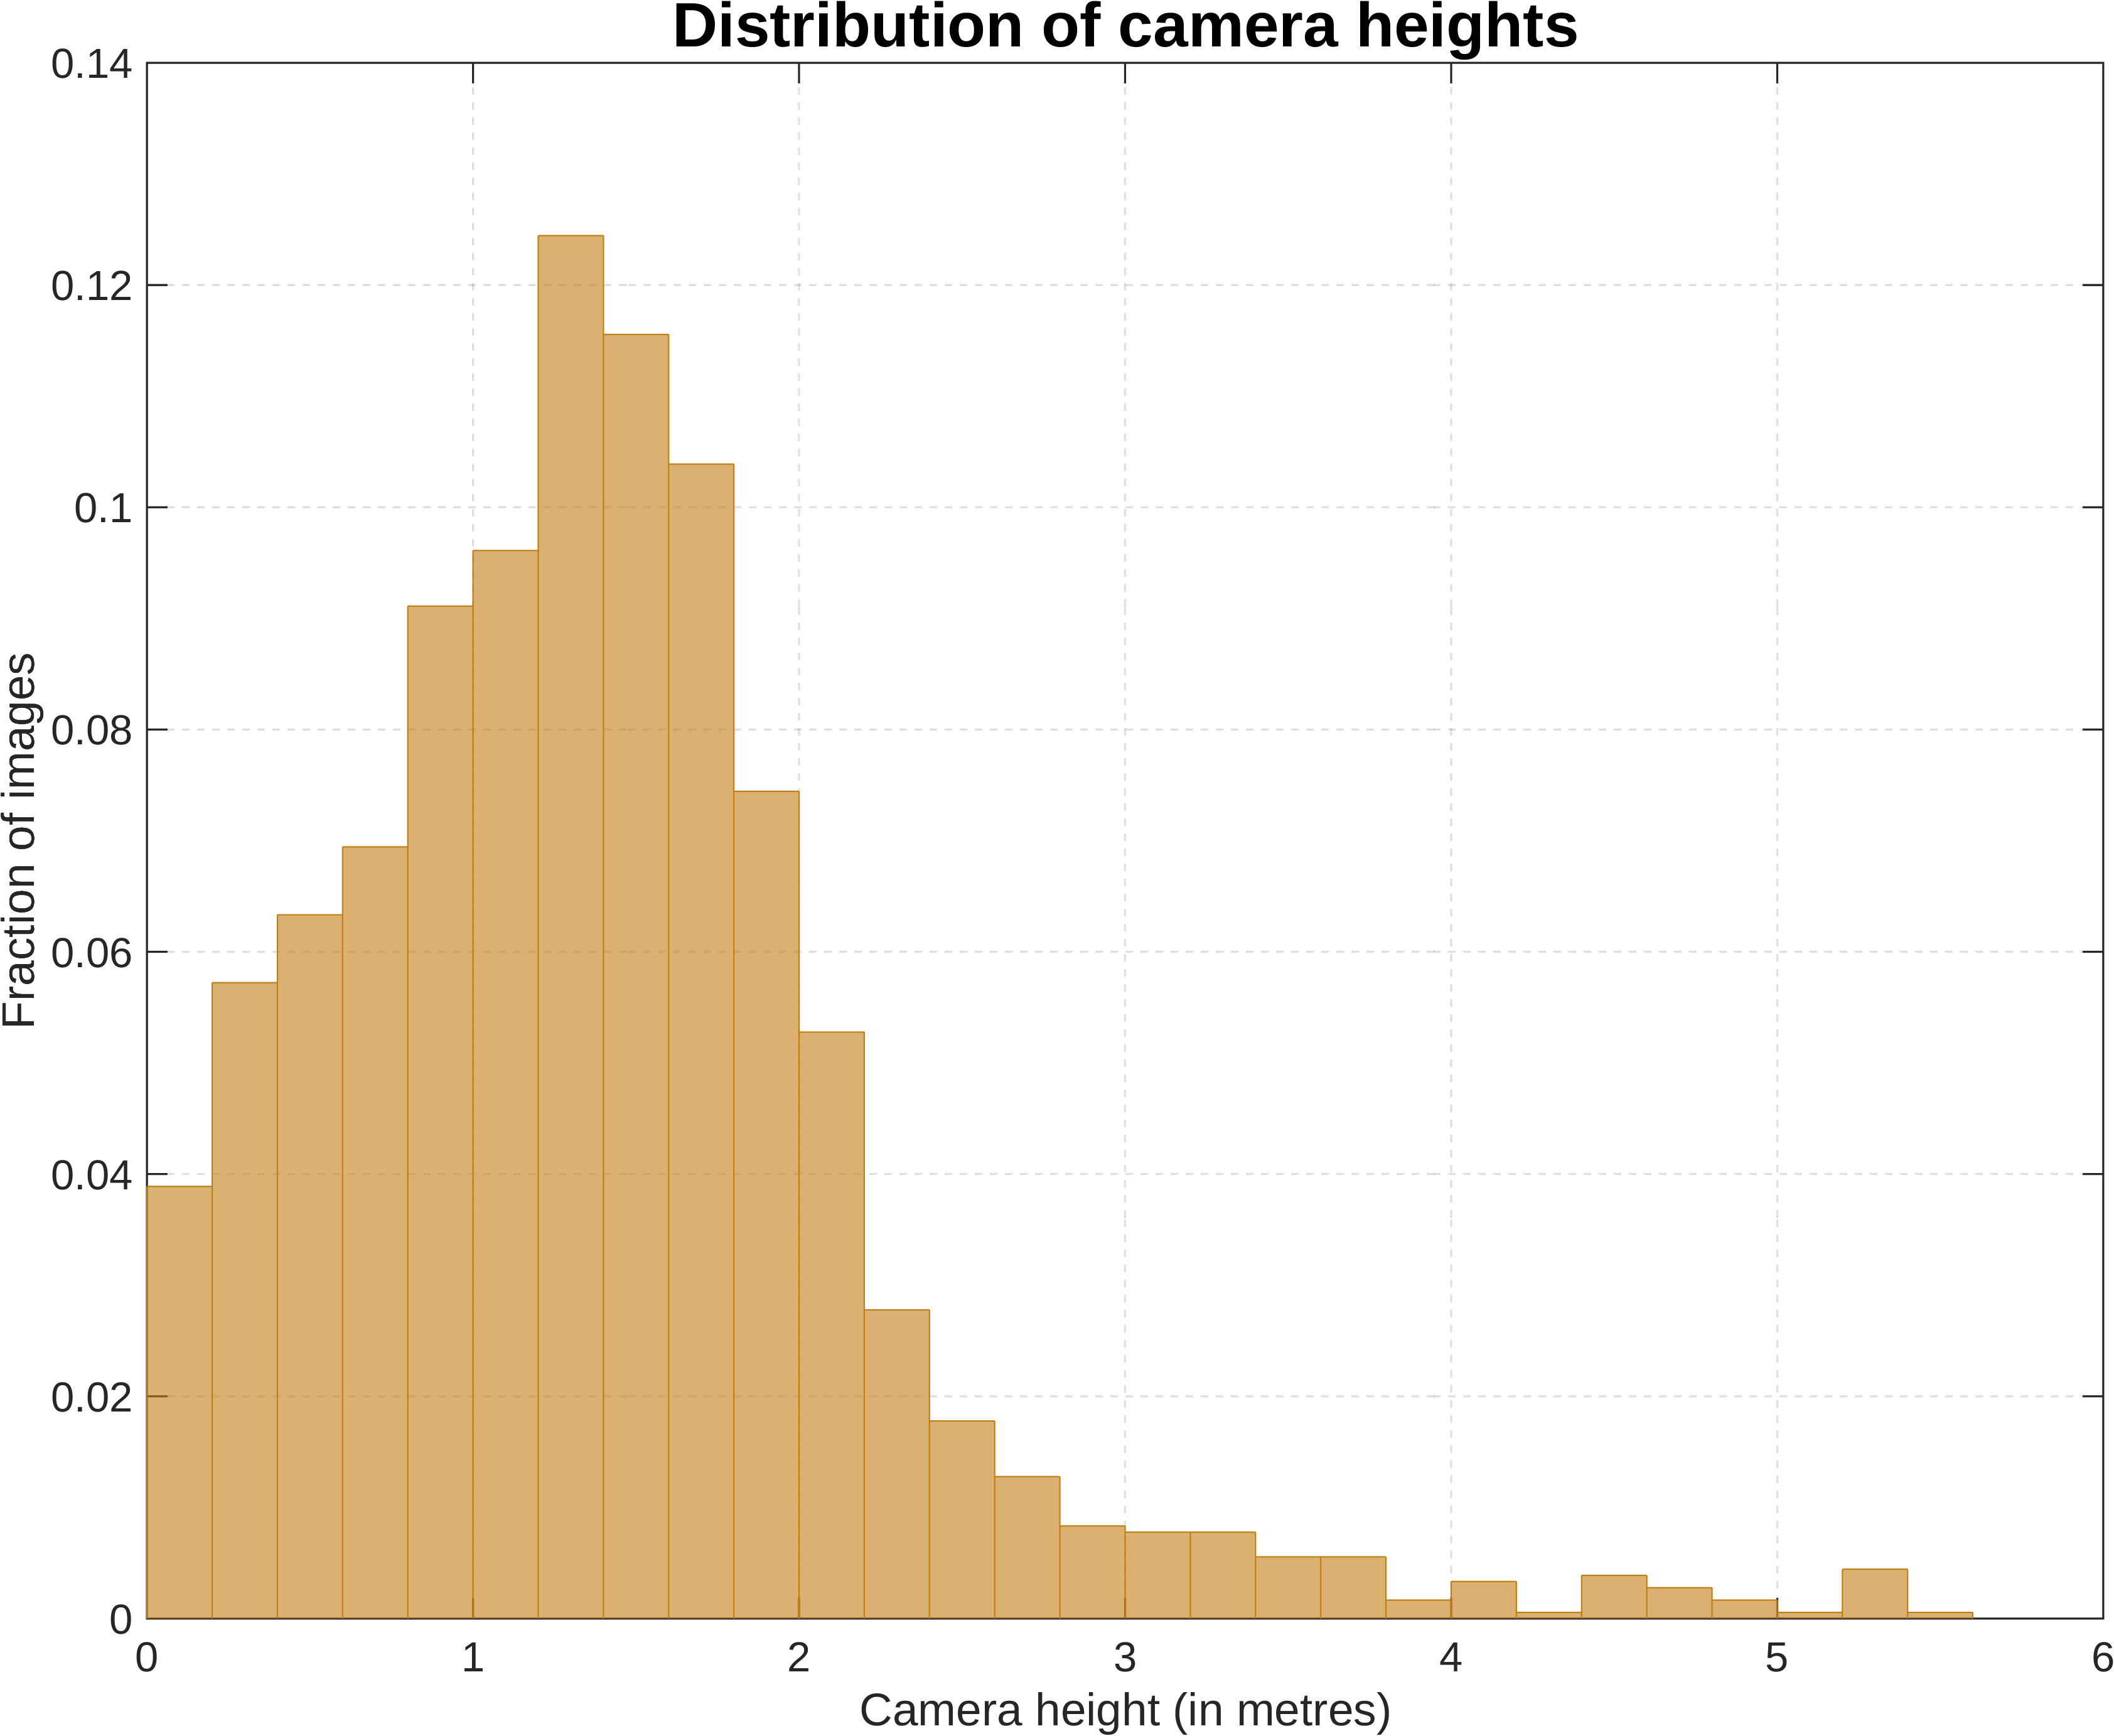
\includegraphics[width=0.95\linewidth]{figures/amodal/heights_pred_choc.png}
    \caption{\figlabel{heightDistr} Distribution of camera heights as inferred on PASCAL VOC. It can be seen that the distribution is peaked around the height at which humans normally take pictures (1.4m) with a long tail.}
  \end{minipage}
  \hfill
  \begin{minipage}{.45\textwidth}
    \centering
    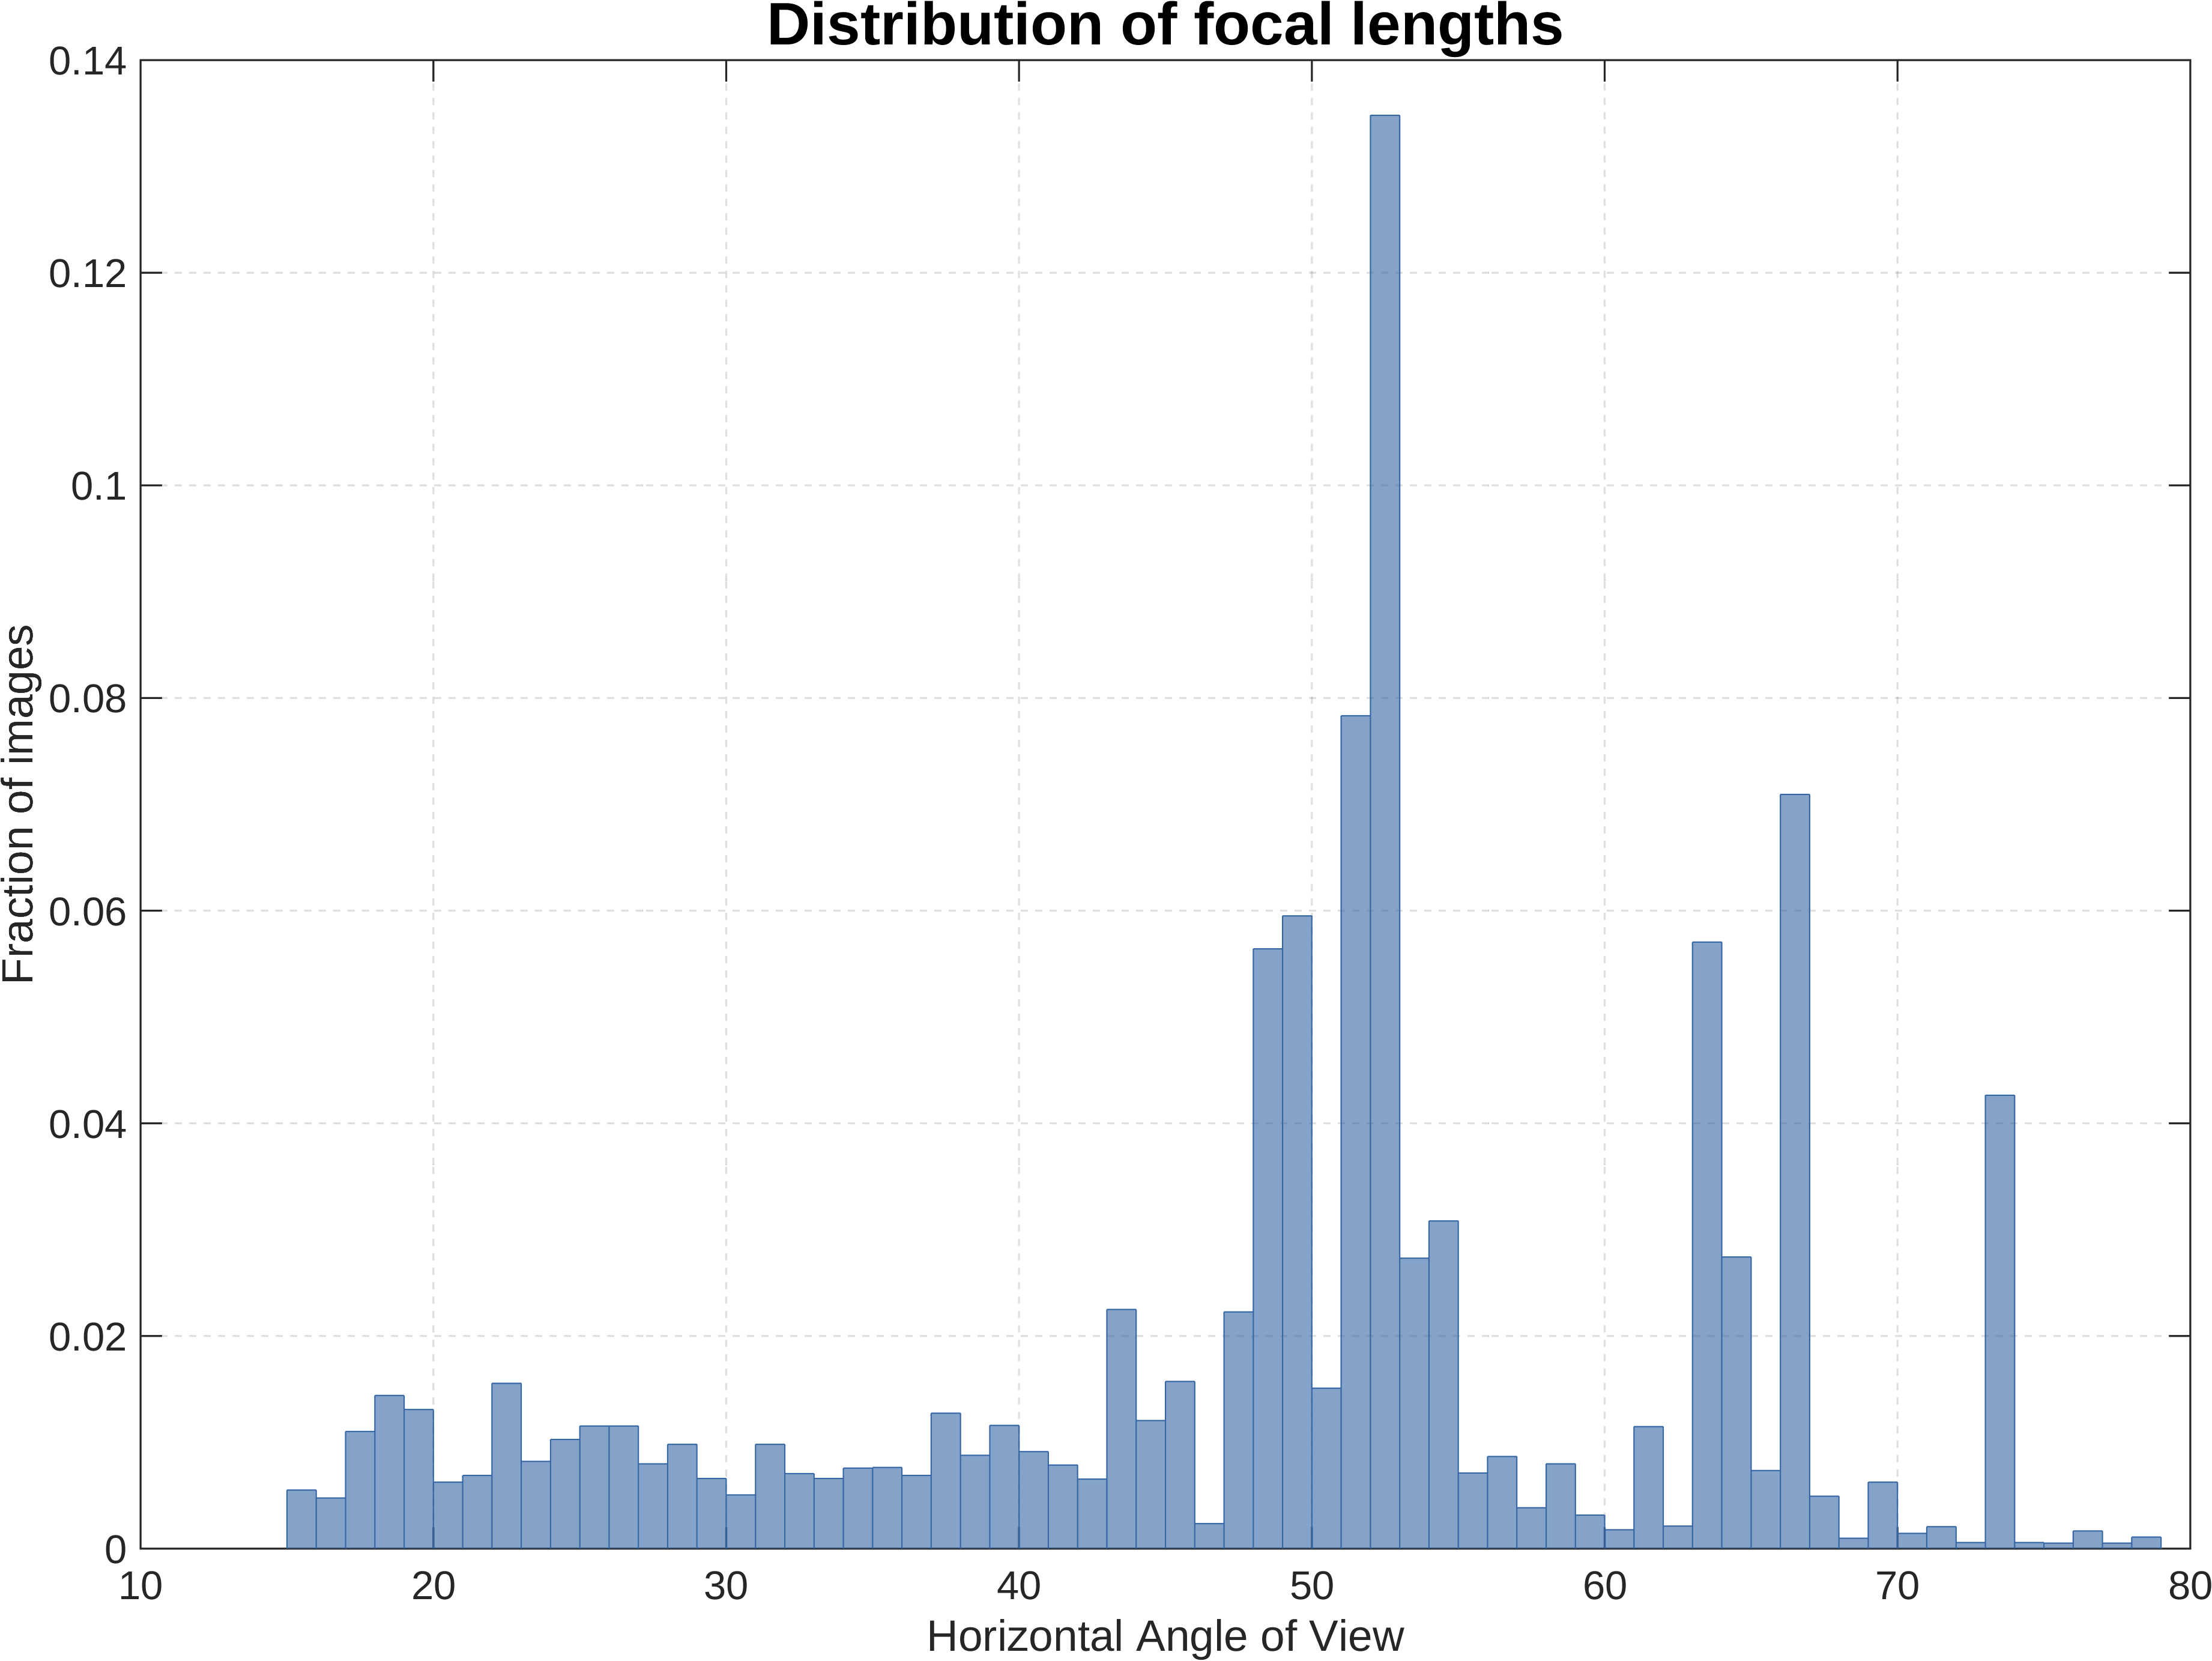
\includegraphics[width=0.95\linewidth]{figures/amodal/fov.png}
    \caption{\figlabel{fovDistr} Distribution of camera focal lengths in the Places dataset shown as horizontal angle of view. The peaks in the distribution correspond to canonical focal lengths in popular wide angle and telephoto lenses. It can be seen that the images cover the full spectrum from wide angle views of scenes (corresponding to the right end of the plot) to close-ups (left end of the histogram).}
  \end{minipage}
  \end{figure}

\paragraph{Results:} The results are shown in \tableref{focal_results} and suggest that focal length can indeed be predicted directly from images, at least approximately, and that pretraining on annotated scene class data makes a good match with this task. Our best model can predict correct focal length quite repeatably  among the top-three and top-five predictions. As baselines, we measure chance performance, and performance when picking the mode of the distribution on the training set -- the bin having most elements. The (unequal) distribution of the focal lengths can be seen in \figref{fovDistr}.


Note that our goal is not high precision of the type that is necessary for high-fidelity reconstruction; we aim for a coarse estimate of the focal length that can be robustly computed from natural images. Our results in this section are a first demonstration that this may be feasible.

\begin{table}
\centering
\resizebox{0.5\linewidth}{!}{
 \begin{tabular}{ l  c  c c}
\toprule
\textbf{Method} & \textbf{top-1} & \textbf{top-3} & \textbf{top-5} \\
\midrule
Chance & 90.0 & 70.0 & 50.0 \\
Mode Selection & 60.2 & 26.4 & 8.7 \\
\midrule
AlexNet-Imagenet & 57.1  & 18.8 & 3.9 \\
VGG-Deep16-Imagenet & 55.8 & 15.9 & 3.3 \\
PlacesNet-Places & \textbf{54.3} & \textbf{15.3} & \textbf{3.1} \\
\bottomrule
  \end{tabular}}
    \caption{\tablelabel{focal_results}Focal length misclassification rate (top-1, top-3 and top-5 predictions) of networks pretrained on object images from Imagenet and the Places dataset. Lower is better.}
\end{table}
\begin{figure}[htb]
  \centering
  \includegraphics[width=\textwidth]{figures/amodal/resultsFig.png}

\caption{\figlabel{resultFig} Amodal bounding box prediction and size estimation results on images in PASCAL VOC. The solid rectangles represent the visible bounding boxes and the dotted lines are the predicted amodal bounding boxes with heights in meters. The horizontal red line denotes the estimated horizon position for the image.}
\end{figure}
\section{Discussion}
We have studied the problem of veridical size estimation in complex natural scenes, with the goal of enriching the visual representations inferred by current recognition systems. We presented techniques for performing amodal completion of detected object bounding boxes, which together with geometric cues allow us to recover relative object sizes, and hence achieve a desirable property of any perceptual system - size constancy. We have also introduced and demonstrated a learning-based approach for predicting focal lengths, which can allow for metrically accurate predictions when standard auto-calibration cues or camera metadata are unavailable. We strived for generality by leveraging recognition. This is unavoidable because the size constancy problem is fundamentally ill-posed and can only be dealt with probabilistically.

We also note that while the focus of our work is to enable veridical size prediction in natural scenes, the three components we have introduced to achieve this goal - amodal completion, geometric reasoning with size constancy and focal length prediction are generic and widely applicable. We provided individual evaluations of each of these components, which together with our qualitative results demonstrate the suitability of our techniques towards understanding real world images at a rich and general level, beyond the 2D image plane.
% \section*{Acknowledgements}
This work was supported in part by NSF Award IIS-1212798 and ONR MURI-N00014-10-1-0933. Shubham Tulsiani was supported by the Berkeley fellowship and Jo\~{a}o Carreira was supported by the Portuguese Science Foundation, FCT, under grant SFRH/BPD/84194/2012. We gratefully acknowledge NVIDIA corporation for the donation of Tesla GPUs for this research.


\end{document}

\section{Untangling Size and Depth}
\seclabel{sizeconstancy}
Monocular cues for depth perception have been well-studied in psychology literature and there are two very important cues which emerge that tie object size and depth -  namely familiar size and relative size. Familiar size is governed by the fact that the visual angle subtended by an object decreases with distance from the observer and prior knowledge about the actual size of the object can be leveraged to obtain absolute depth of the object in the scene. Relative size, on the other hand, helps in explaining relative depths and sizes of objects - if we know that two objects are of similar sizes in the real world, the smaller object in the image appears farther. Another simple cue for depth perception arises due to perspective projection - an object further in the world appears higher on the image plane. Leveraging these three cues, we show that one can estimate real world object sizes from just images. In addition to object sizes, we also estimate a coarse viewpoint for each image in the form of the horizon and camera height. 

The main idea behind the algorithm is to exploit pairwise size relationships between instances of different object classes in images. As we will show below, given support points of objects on the ground and some rough estimate of object sizes, one can estimate the camera height and horizon position in the image - and as a result relative object depths. And in turn, given object heights in the image and relative depths, one can figure out the real world object scale ratios. Finally, exploiting these pairwise size evidences across images, we solve for absolute real world sizes (upto a common scale factor or the metric scale factor). Note that we use size and height interchangeably here as our notion of object size here actually refers to the object height.
% Perspective projection figure
\begin{figure}
  \centering
  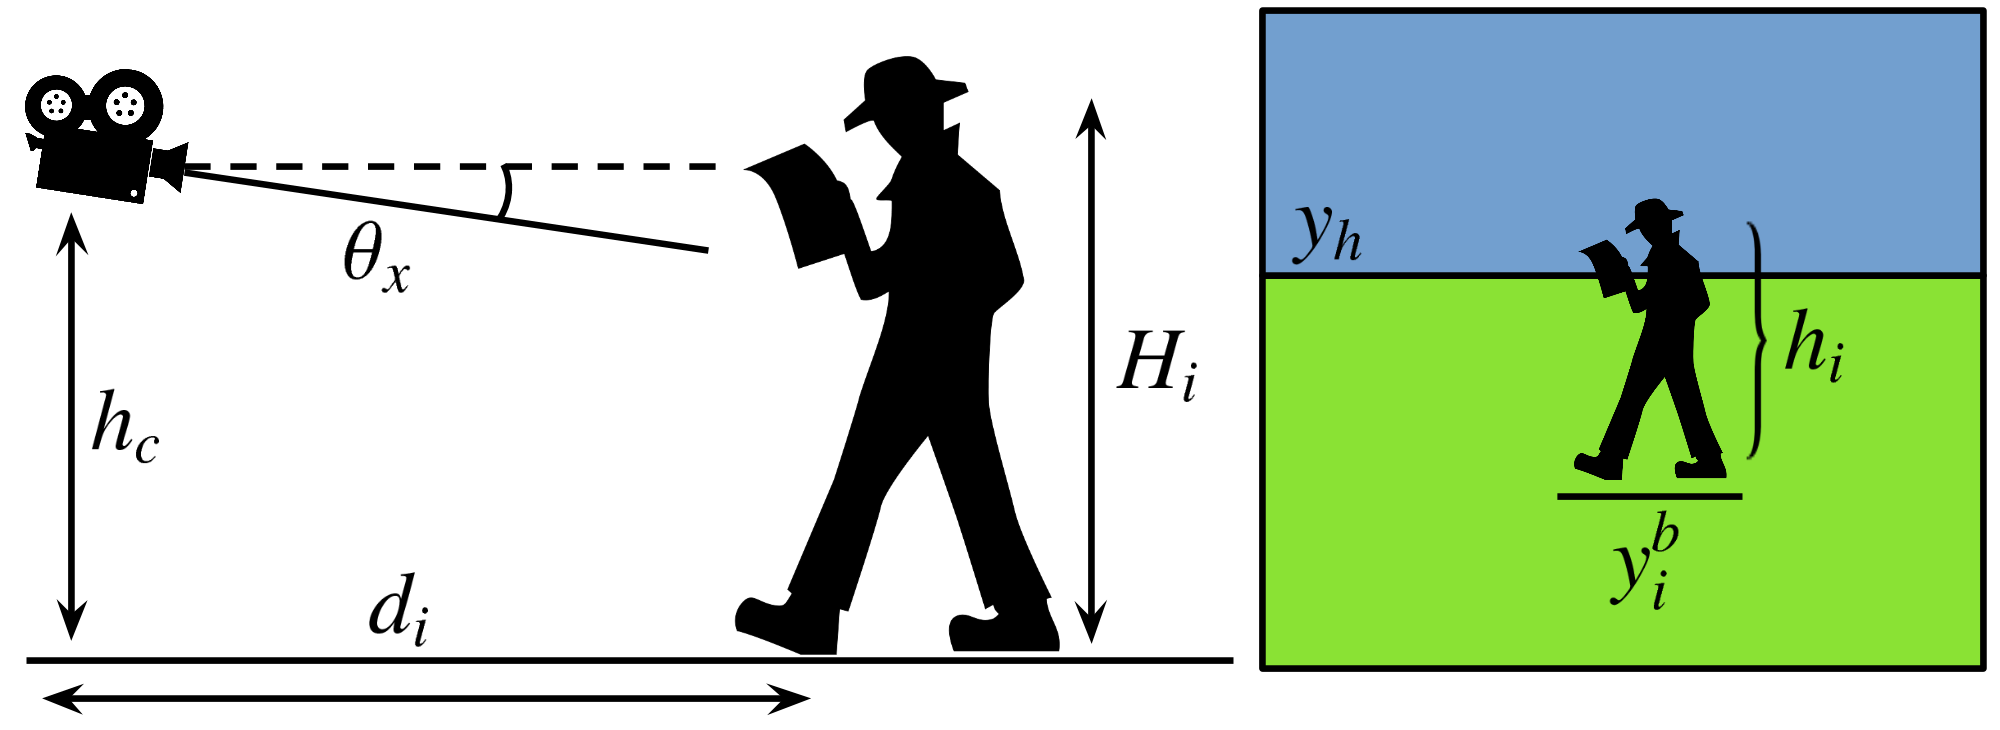
\includegraphics[width=.9\textwidth]{figures/amodal/Perspective.png}
  \caption{\figlabel{perspective} Toy example illustrating our camera model and parameters. Please refer to the text for detailed explanations. }
\end{figure}

\paragraph{Camera Model:} We use a simplified perspective camera model similar to Hoiem \etal~\cite{hoiem2008putting}. Let $f$ be the focal length of the camera, $\theta_x$ the camera tilt angle along the x-axis, $h_c$ the height of the camera, $y_h$ be the horizon position in the image, $y_i^b$ be the ground support point for the $i^{th}$ object in the image and $d_i$ be the distance of the $i^{th}$ object from the camera along the camera axis ($z$ axis). We assume that the images have been corrected for camera roll and all pixel co-ordinates are with respect to the optical center (assumed to be center of the image). \figref{perspective} provides a toy illustration of our model and parameters.

Assuming that the world frame is centered at the camera with its $y$ axis aligned with the ground, the projection of a world point $\mathbf{X} = (X_w,Y_w,Z_w)$ in the image in homogeneous co-ordinates is given by:
\bes
\begin{bmatrix}
x \\
y \\
1
\end{bmatrix} = \frac{1}{Z_w}
\begin{bmatrix}
f & 0 & 0\\
0 & f & 0\\
0 & 0 & 1
\end{bmatrix}
\begin{bmatrix}
1 & 0 & 0 & 0 \\
0 & \cos\theta_x & \sin\theta_x & 0 \\
0 & -\sin\theta_x & \cos\theta_x & 0 \\
\end{bmatrix}
\begin{bmatrix}
X_w \\
Y_w \\
Z_w \\
1
\end{bmatrix}
\ees
For a world point corresponding to the ground contact point of object $i$, given by $(X_w,-h,d_i)$, its corresponding $y$ co-ordinate in the image $y_i^b$ is given by:
$
y_i^b = f\frac{(-h_c/d_i + \tan\theta_x)}{1+(h_c/d_i)\tan\theta_x}
$
Under the assumption of the tilt angle being small ($\tan\theta_x \approx \theta_x$) and height of the camera being not too large compared to object distance ($h\theta_x \ll d_i$), our approximation is 
\be
\eqlabel{groundEq}
y_i^b = -\frac{fh_c}{d_i} + f\theta_x
\ee
Here $f\theta_x$ corresponds to the position of the horizon ($y_h$) in the image. Repeating the above calculation for the topmost point of the object and subtracting from \eqref{groundEq}, we obtain
\be 
\eqlabel{sizeEq}
h_i = \frac{fH_i}{d_i}
\ee
where $h_i$ refers to the height of the object in the image and $H_i$ is the real world height of the object.
Our model makes some simplifying assumptions about the scene namely, objects are assumed to rest on the same horizontal surface (here, the ground) and camera tilt is assumed to be small. We observe that for the purpose of size inference, these assumptions turn out to be reasonable and allow us to estimate heights of objects fairly robustly.

% Algorithm box for size estimation
\begin{algorithm}[h]
\caption{Object Size Estimation}
\begin{algorithmic}
\Initialize{Initial size estimates $\mathbf{H}$ and cluster assignments}
\While {not converged}
\ForAll{images $k \in $ Dataset }
\State $(h_c,y_h) \gets $ SolveLeastSquares($y_b,h,\mathbf{H}$)
\ForAll{pairs $(i,j)$ of objects in $k$}
\State $\frac{H_i}{H_j} \gets \frac{h_i}{h_j}\frac{y_j^b-y_h}{y_i^b-y_h}$\Comment{$(1)$}
\EndFor
\EndFor
\State $\log \mathbf{H} \gets$ least squares with pairwise constraints ($1$)
\State GMM cluster log scales ($\log \mathbf{H}$)
\State Reassign objects to clusters
\EndWhile
\end{algorithmic}
\label{alg:sizeEstimation}
\end{algorithm}

\paragraph{Inferring Object Sizes:} 
The important observation here is that the sizes of objects in an object category are not completely random - they potentially follow a multimodal distribution. For example, different subcategories of boats may represent the different modes of the size distribution. Given some initial sizes and size cluster estimates, our algorithm for size estimation (Algorithm \ref{alg:sizeEstimation}) works by estimating the horizon and camera height per image (by solving a least squares problem using \eqref{groundEq} and \eqref{sizeEq} for all the objects in an image). With the horizon and height estimated per image, we obtain pairwise height ratios $\frac{H_i}{H_j} = \frac{h_i}{h_j}\frac{y_j^b-y_h}{y_i^b-y_h}$ for each pair of objects in an image. We obtain multiple such hypotheses across the dataset which we use to solve a least squares problem for $\log \mathbf{H}$ - the log height for each size cluster. Finally, we cluster the log sizes obtained in the previous step to obtain new size clusters and iterate. Note that $\mathbf{H}$ refers to the vector with heights of various classes and $H_i$ refers to the real world size of the $i^{th}$ object.

This particular model is equivalent to solving a latent variable model where the latent variables are the cluster memberships of the instances, the estimated variables are heights corresponding to the size clusters and the horizon and camera height for each image. The loss function we try to minimize is the mean squared error between the ground contact point predicted by the model and the amodal bounding box. Finally, the log of the object heights are assumed to be a Gaussian mixture. This final assumption ties in elegantly with psychophysics studies which have found that our mental representation of object size (referred to as assumed size~\cite{ittelson1951size,baird1963retinal,epstein1963influence}) is proportional to the logarithm of the real world object size~\cite{konkle2011canonical}.

Our image evidences in the above procedure include the ground support points and heights for all the objects in the image. Note that amodal bounding boxes for objects provide us exactly this information. They account for occlusions and truncations and give us an estimate of the full extent of the object in the image. The above algorithm with occluded/truncated visible bounding boxes would fail miserably and we use our amodal bounding box predictor to first ``complete'' the bounding boxes for us before using our size inference algorithm to infer object heights.

\begin{figure}[htb]
  \centering
  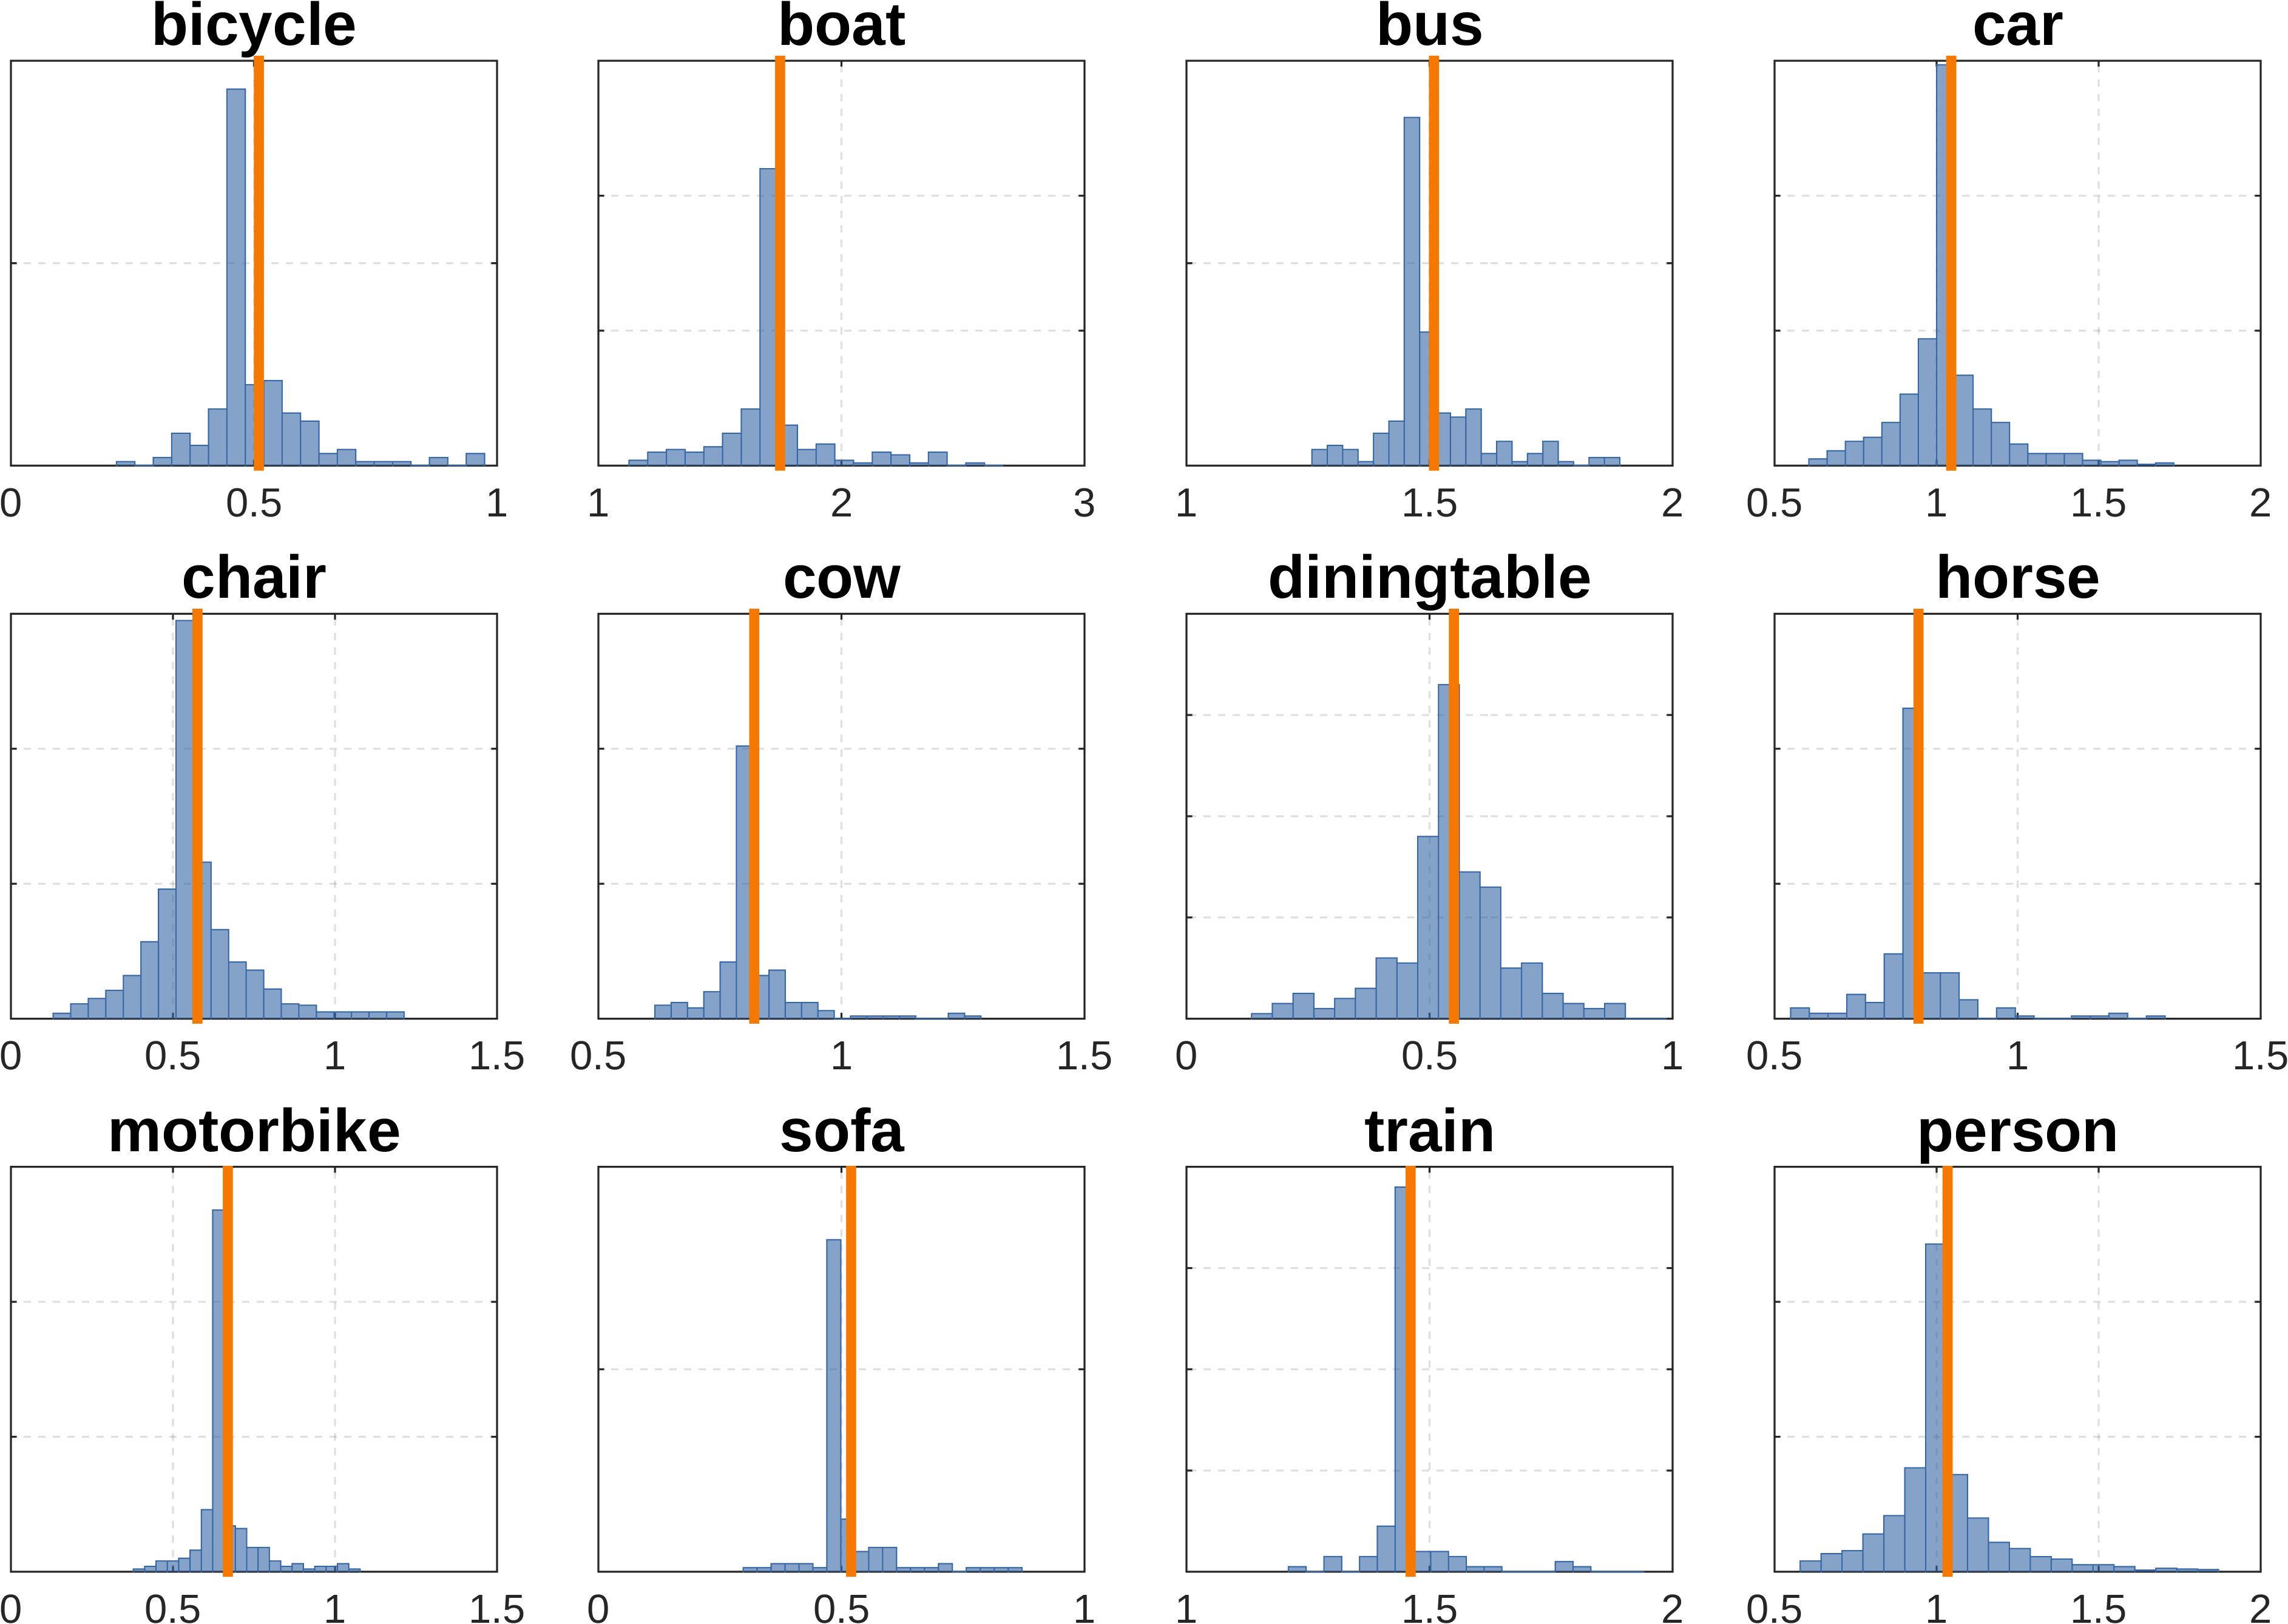
\includegraphics[width=.9\textwidth]{figures/amodal/size_PascalVal_pred.png}
  \caption{\figlabel{pascalSizes} Inferred log size distributions of 12 object categories on PASCAL VOC. We use our class agnostic amodal bounding box predictor to predict amodal boxes for all instances in VOC 2012 \textit{det-val} and use them with our object size estimation system to estimate size distributions for various categories. The plots above show distributions of the log size with the mean size being shown by the orange line.}
\end{figure}

\paragraph{Inferring Object Size Statistics on PASCAL VOC:} We used our size estimation system on PASCAL VOC to estimate size distributions of objects. First, we use our class agnostic amodal bounding box predictor on ground truth visible bounding boxes of all instances on VOC 2012 \textit{det-val} to ``upgrade'' them to amodal boxes. We initialize our system with a rough mean height for each object class obtained from internet sources (Wikipedia, databases of cars etc.) and run our size estimation algorithm on these predicted amodal boxes. \figref{pascalSizes} shows the distributions of log sizes of objects of various categories in PASCAL VOC. Most categories exhibit peaky distributions with classes such as ``boat'' and ``chair'' having longer tails owing to comparatively large intra class variation. Note that we experimented with using multiple size clusters per class for this experiment but the peaky, long tailed nature of these distributions meant that a single Gaussian capturing the log size distributions sufficed. In addition to inferring object sizes, we also infer the horizon position and height of the camera. The median height of the camera across the dataset was 1.4 metres (roughly the height at which people take images) and also exhibited a long tailed distribution (please refer to supplementary for details). Some examples of amodal bounding boxes estimated for all instances from visible bounding boxes and horizons are shown in \figref{resultFig}.



\begin{figure}[htb]
  \centering
  \includegraphics[width=\textwidth]{figures/amodal/resultsFig.png}

\caption{\figlabel{resultFig} Amodal bounding box prediction and size estimation results on images in PASCAL VOC. The solid rectangles represent the visible bounding boxes and the dotted lines are the predicted amodal bounding boxes with heights in meters. The horizontal red line denotes the estimated horizon position for the image.}
\end{figure}
\section{Scenes and Focal Lengths}
\seclabel{sceneFocal}
The focal length of a camera defines its field of view and hence determines how much of a scene is captured in an image taken by the camera. It is an important calibration parameter for obtaining metric, as opposed to projective, measurements from images. It is usually calibrated using multiple images of a known object \cite{zhang2000flexible}, such as a chessboard, or as part of bundle adjustment \cite{triggs2000bundle}, from multiple images of realistic scenes. Well known existing approaches require a minimum set of vanishing lines  \cite{wang1991camera} or exploit Manhattan-world assumptions \cite{caprile1990using}. These techniques are very precise and elegant, but not generally applicable (e.g. beach or forest images, \etc).

We propose instead a learning approach that predicts focal length based on statistical dependencies between scene classes and fields of view. Given the same scene, images taken with large focal lengths will have fewer things in them than those captured with small focal lengths and this provides a cue for determining focal length. However certain scenes also have more things than others. This ambiguity can be resolved by training a predictor with many images of each scene class, taken with different focal lengths. 

Additionally, certain scenes tend to be pictured with preferred focal lengths. As an example, consider a scene class of ``pulpits". If a picture of a pulpit is taken with a short focal length, then the whole church will be visible and that image will not be tagged as a pulpit scene. In order for a pulpit to be dominant in a picture taken with a short focal length camera, then the photographer would have to be unnaturally close to it. 

\paragraph{Data:} We use the Places database \cite{zhou2014learning}, a large dataset that provides a dense sampling of scenes in natural images: it has $205$ scene classes, as diverse as \textit{swimming pool} and \textit{rope bridge}, and $2.5$ million images. We were able to scrape focal length metadata from EXIF tags of approximately $20$k examples, on average 100 per class, and split these into a training set having $15$k and a validation set of $5$k images. 

\paragraph{Learning:} We considered the problem of predicting the ratio of the focal length to the camera sensor width, which when multiplied by the size of the image in pixels gives the desired the focal length in pixels. We clustered the logarithm of this ratio into $10$ bins using k-means and formulated the prediction problem as classification, using a softmax loss. Images in the bin with highest and smallest focal length ratio are shown in \figref{focal_lengths}. We experimented finetuning different popular convolutional networks, including two trained on Imagenet classification -- AlexNet \cite{krizhevsky2012imagenet} and VGG-Deep16 \cite{simonyan2014very} -- and a network trained on the Places scenes -- the PlacesNet \cite{zhou2014learning}.

\begin{figure}[htb!]
  \centering
  \includegraphics[width=0.32\textwidth]{figures/amodal/highest4}
  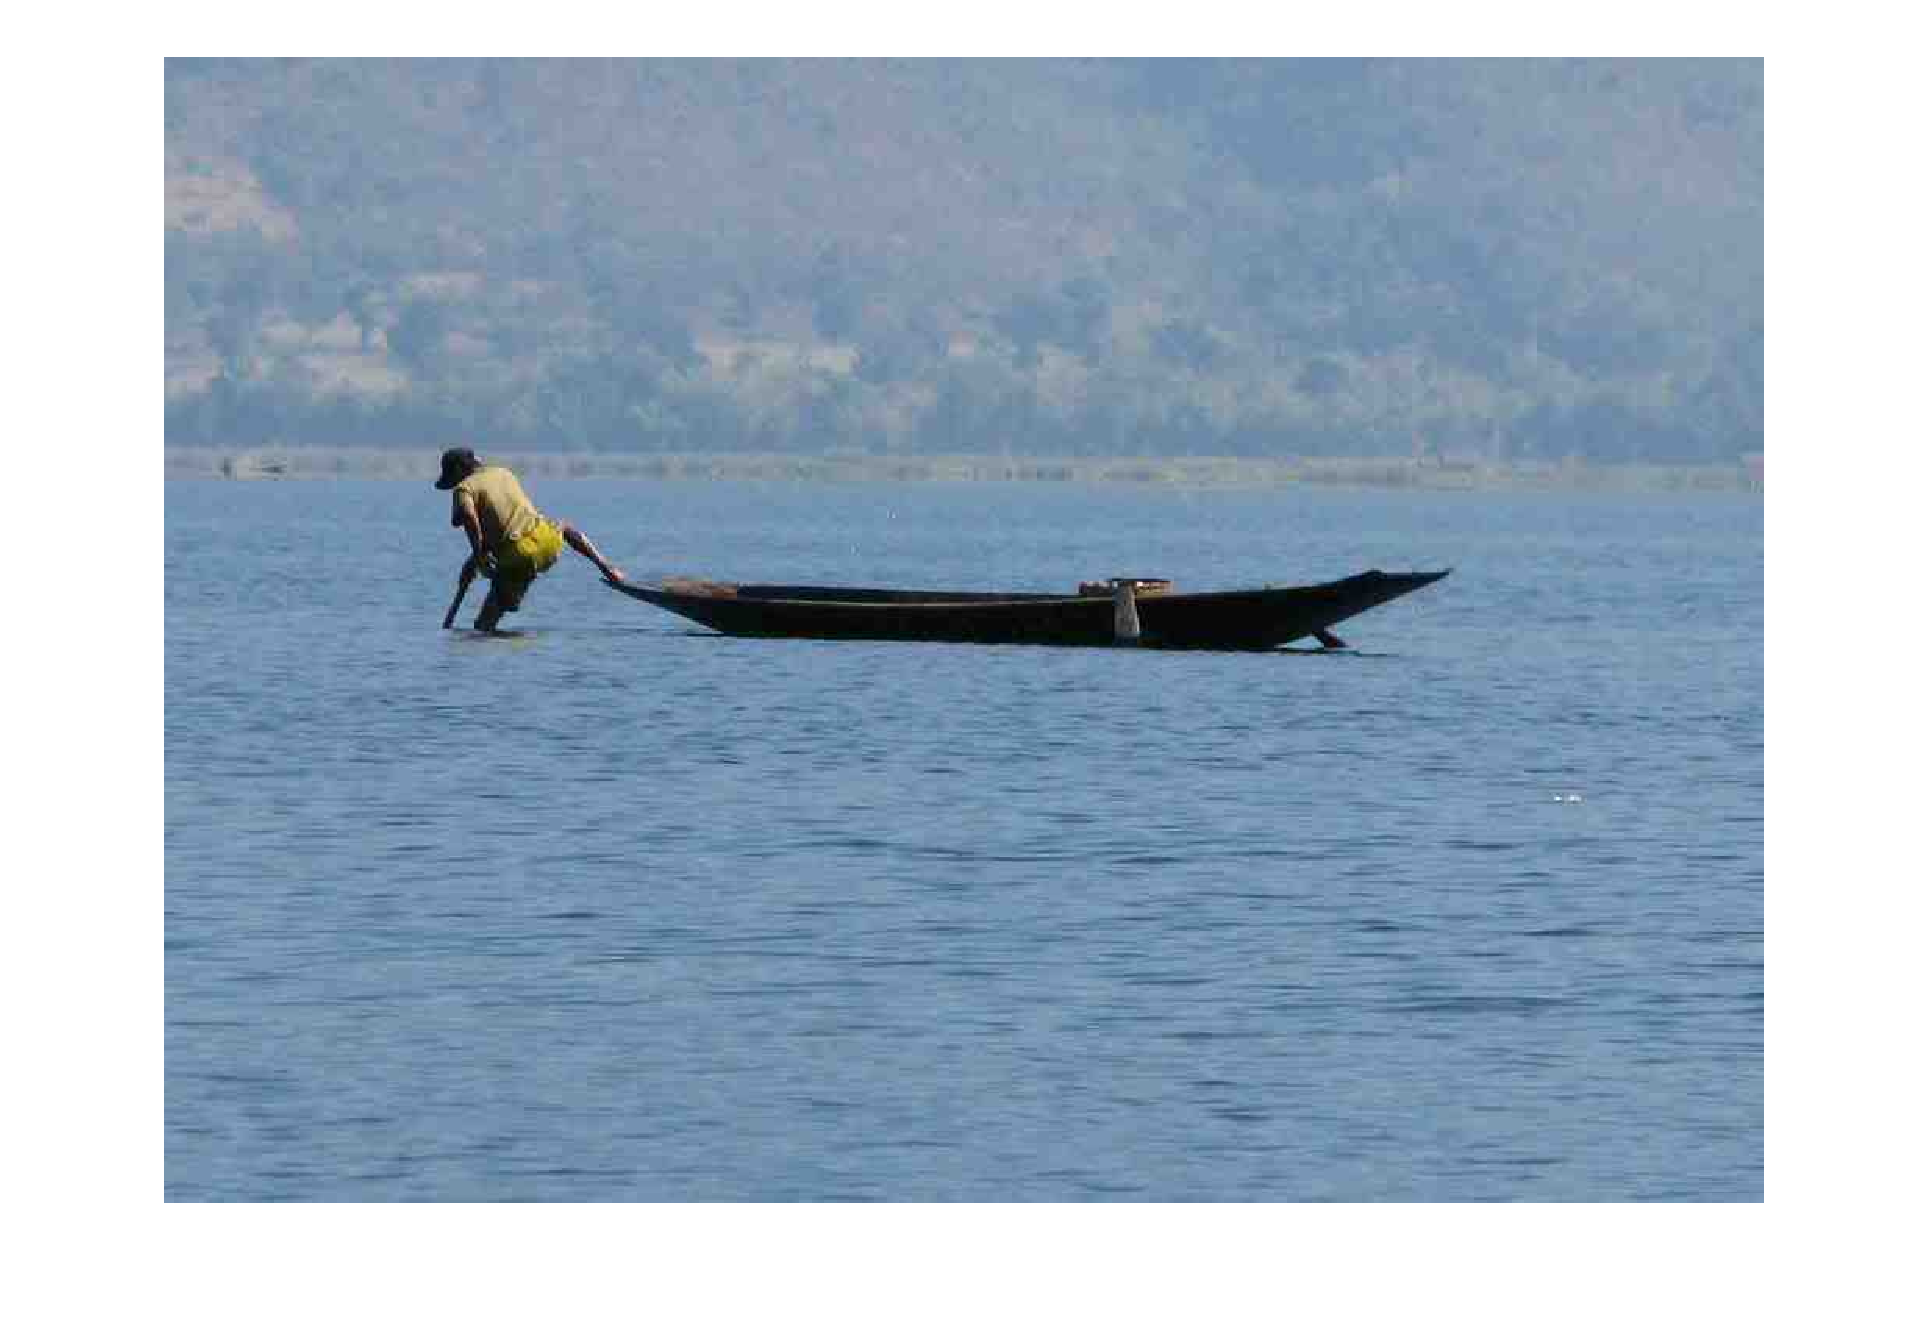
\includegraphics[width=0.32\textwidth]{figures/amodal/highest3}  
  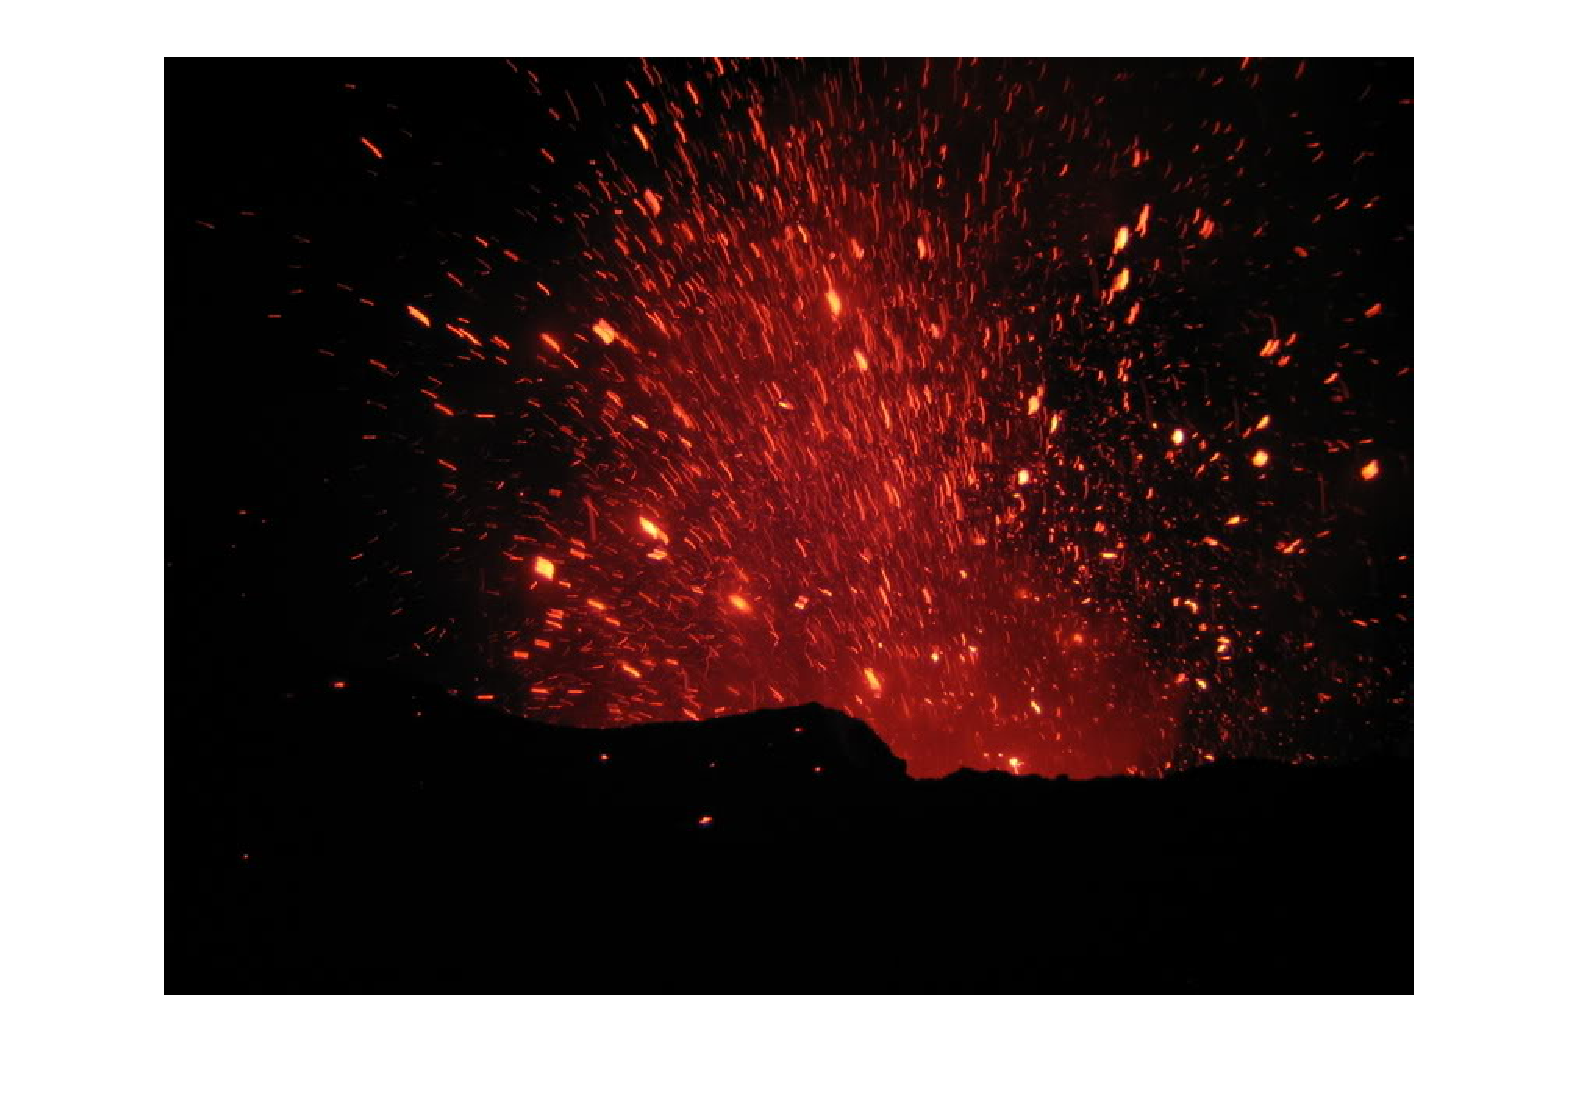
\includegraphics[width=0.32\textwidth]{figures/amodal/highest6}  
  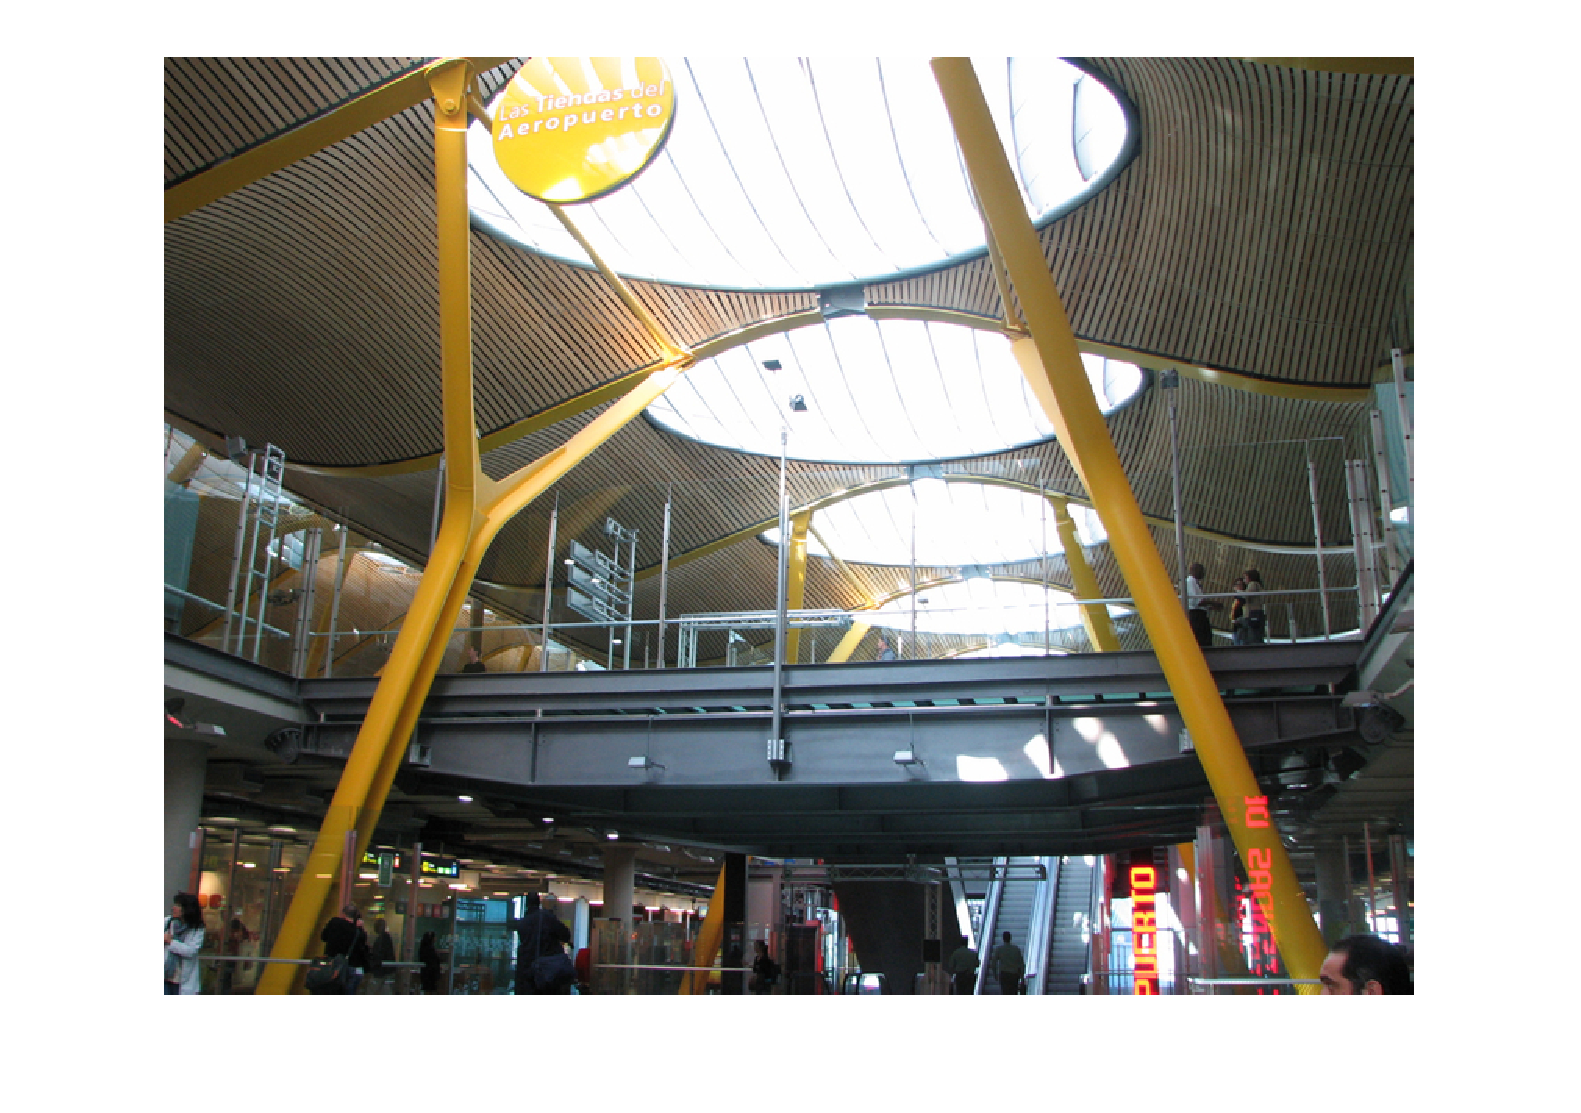
\includegraphics[width=0.32\textwidth]{figures/amodal/lowest1}
  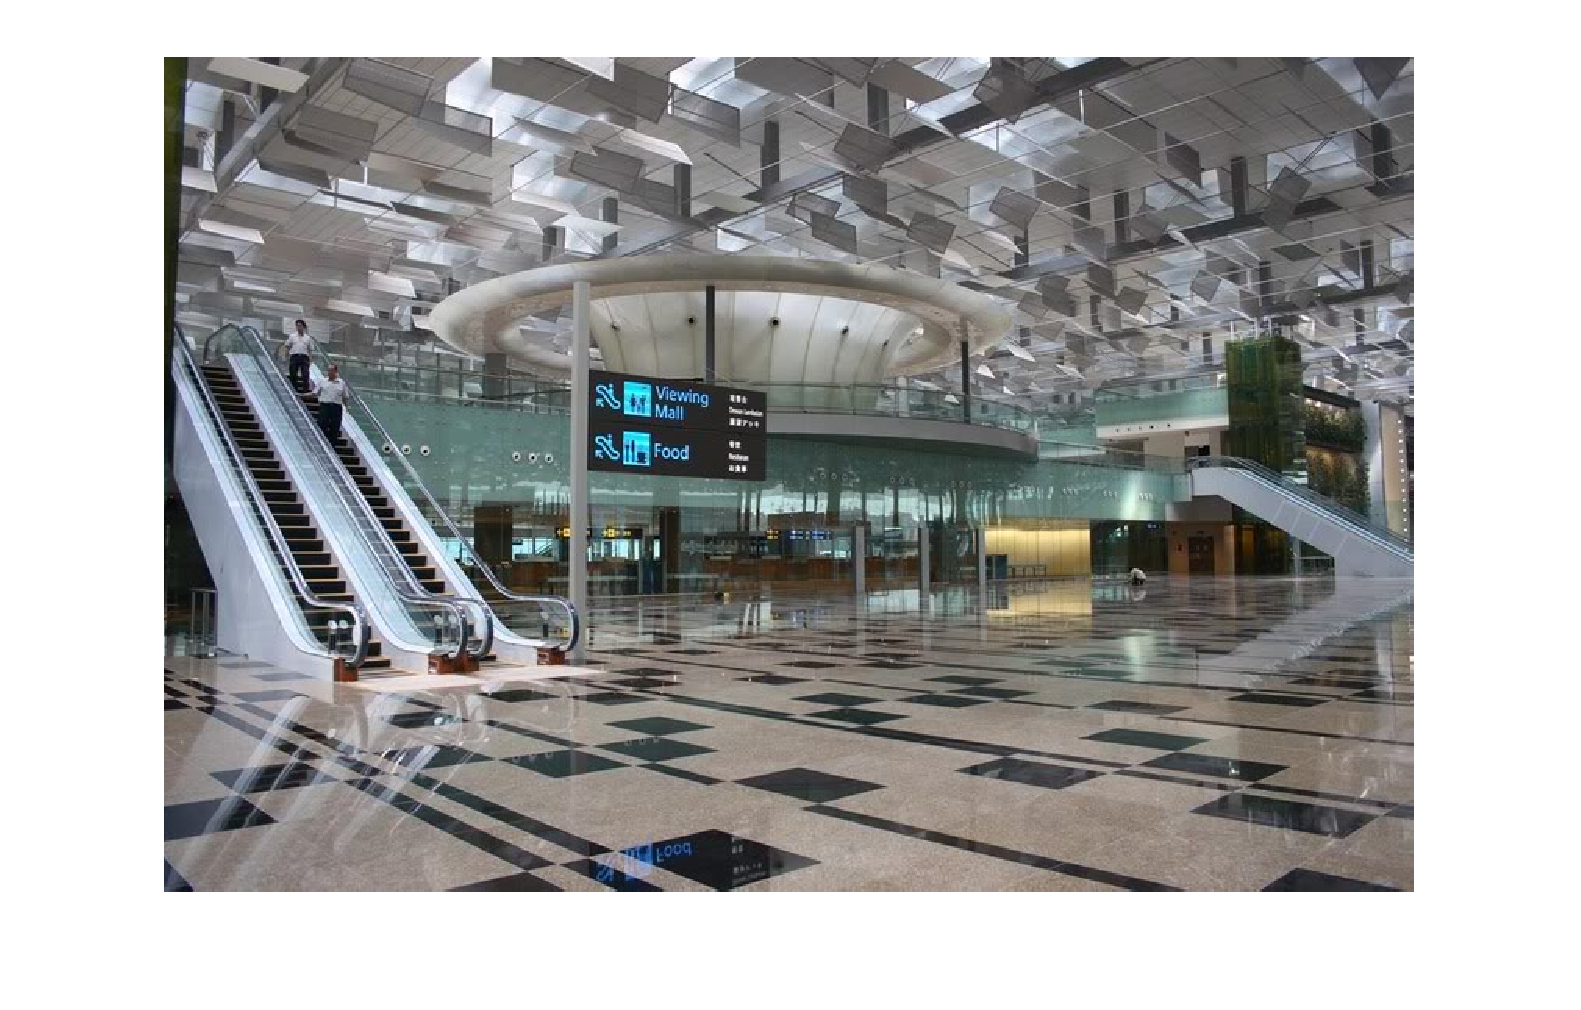
\includegraphics[width=0.32\textwidth]{figures/amodal/lowest3}  
  \includegraphics[width=0.32\textwidth]{figures/amodal/lowest7}
  \caption{\figlabel{focal_lengths} Example images from the Places dataset from clusters with the largest (up) and smallest (down) focal lengths. Note how images with small focal lengths tend to be more cluttered. A pattern we observed is that dangerous or unaccessible scenes, such as those having volcanos, wild animals and boats tend to be captured using very-high focal lengths,  which is rational.}
\end{figure}

\begin{figure}[htb!]
  \centering
  \begin{minipage}{.45\textwidth}
    \centering
    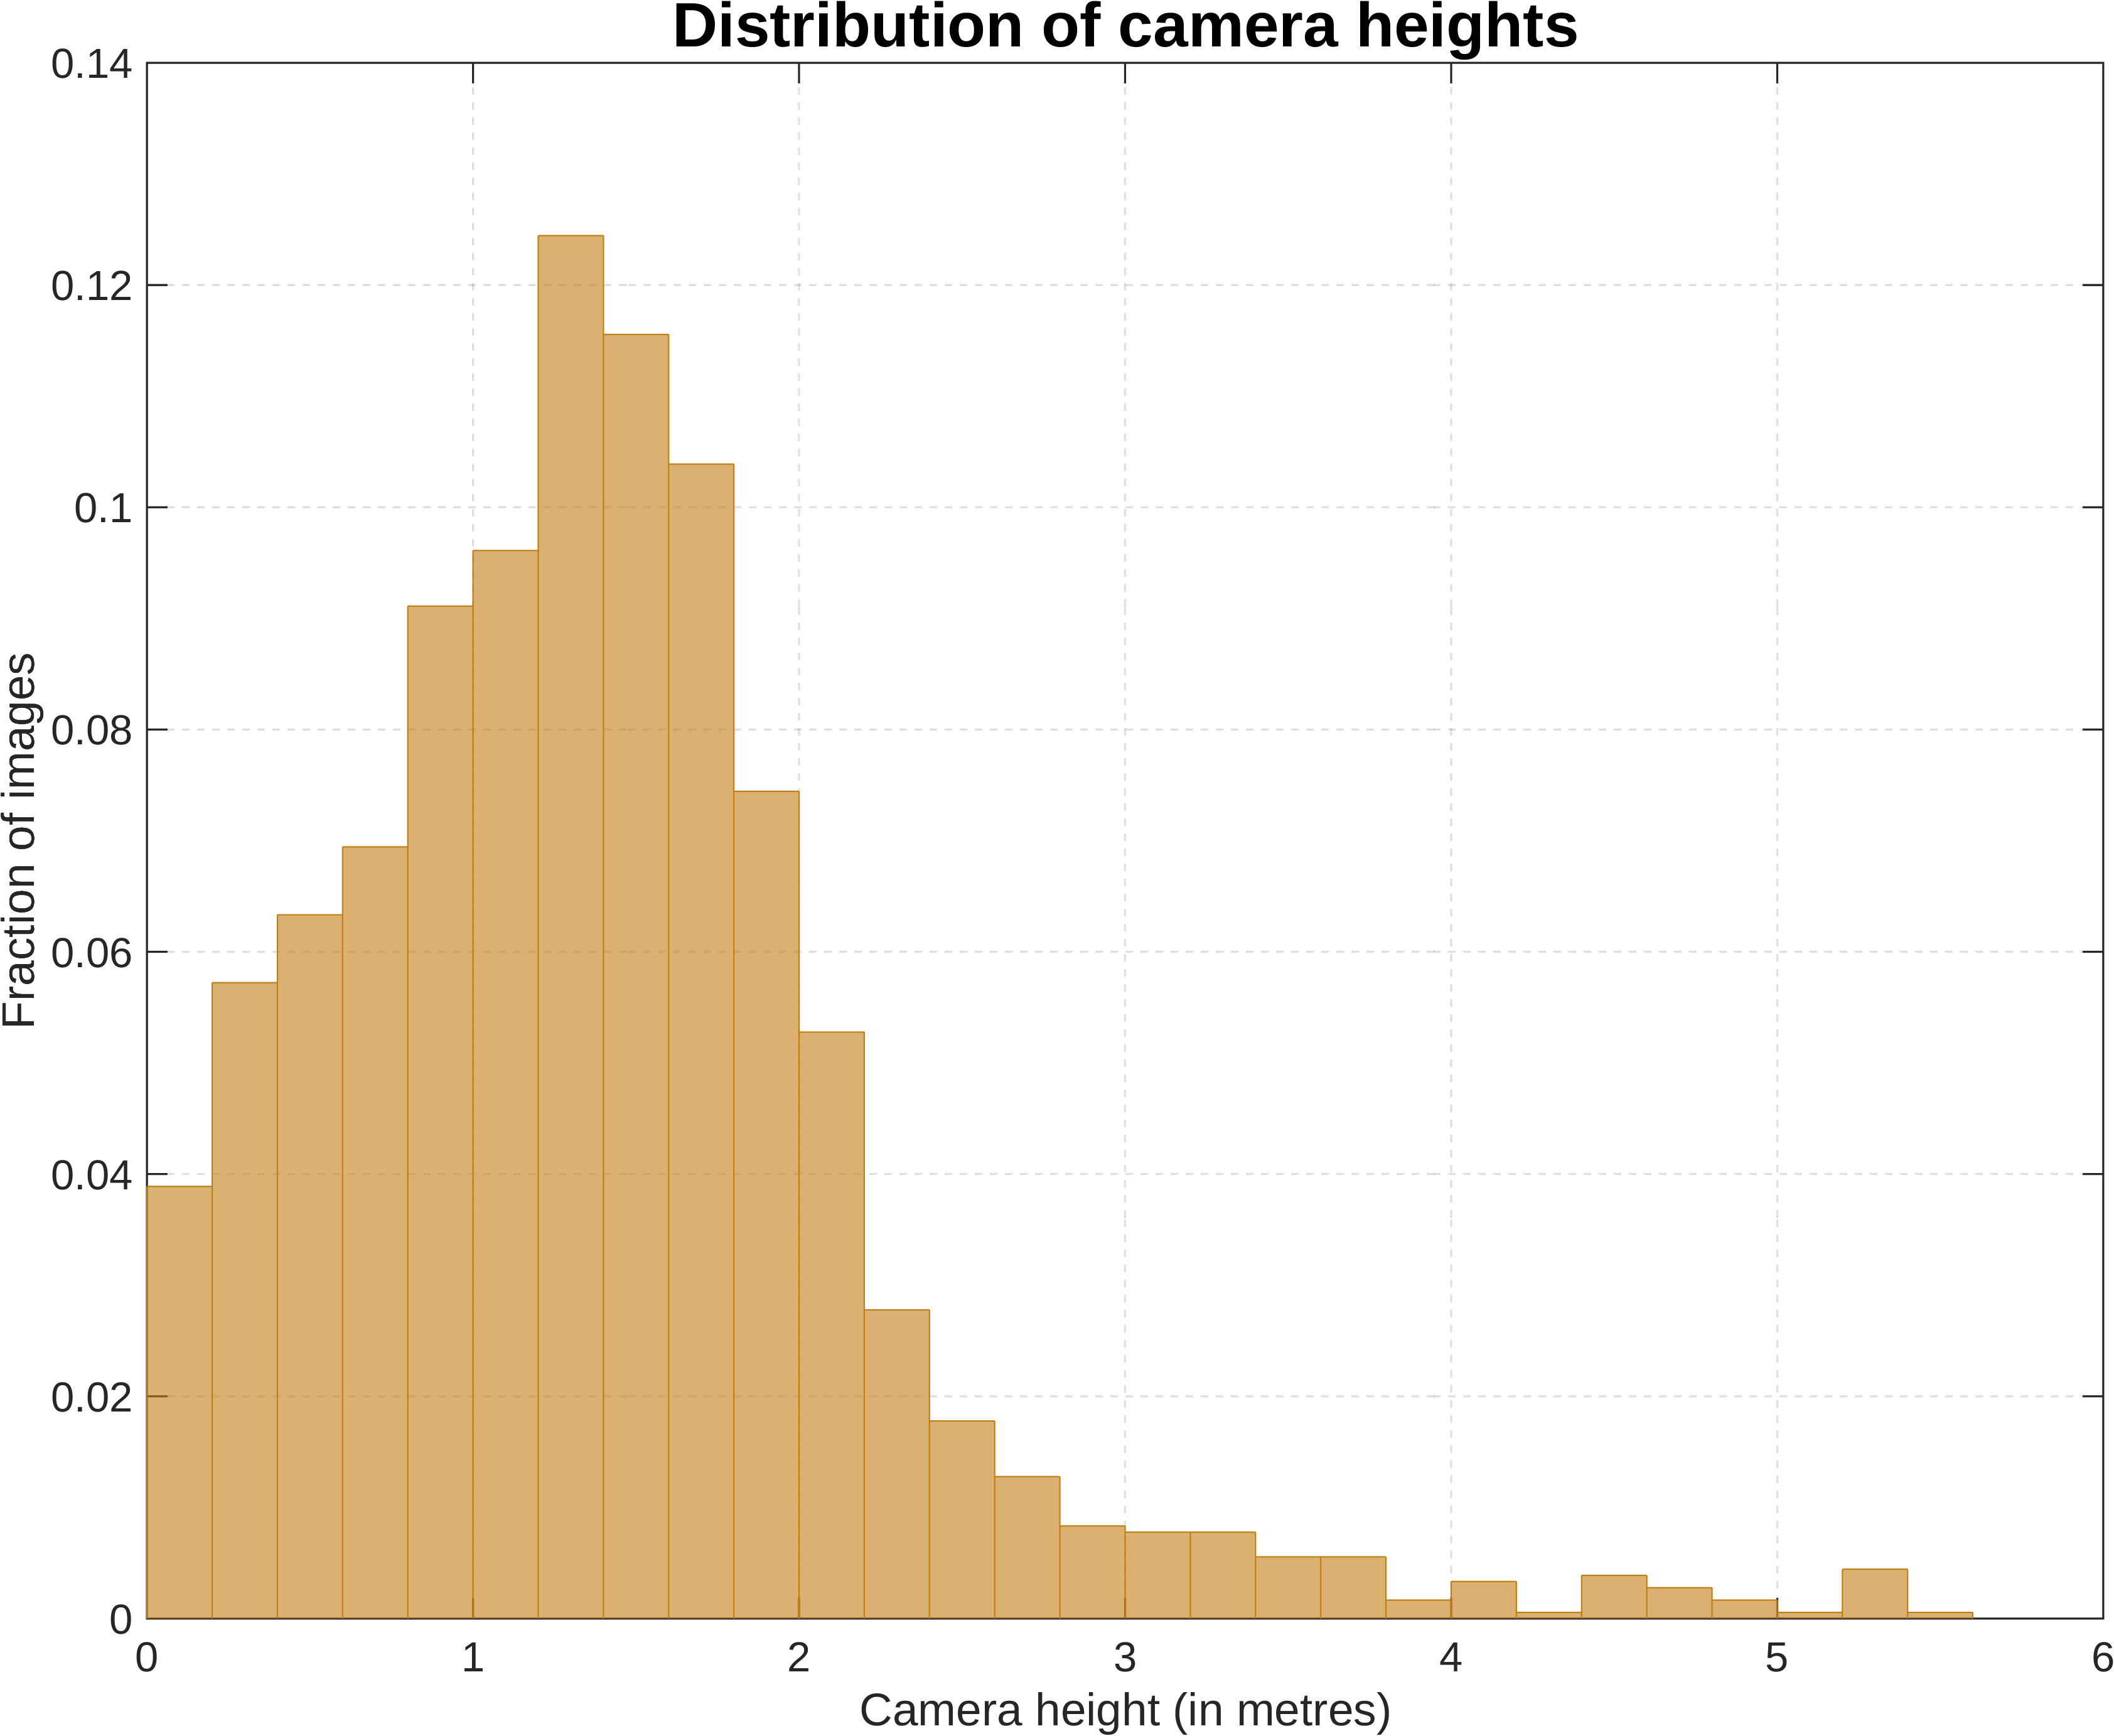
\includegraphics[width=0.95\linewidth]{figures/amodal/heights_pred_choc.png}
    \caption{\figlabel{heightDistr} Distribution of camera heights as inferred on PASCAL VOC. It can be seen that the distribution is peaked around the height at which humans normally take pictures (1.4m) with a long tail.}
  \end{minipage}
  \hfill
  \begin{minipage}{.45\textwidth}
    \centering
    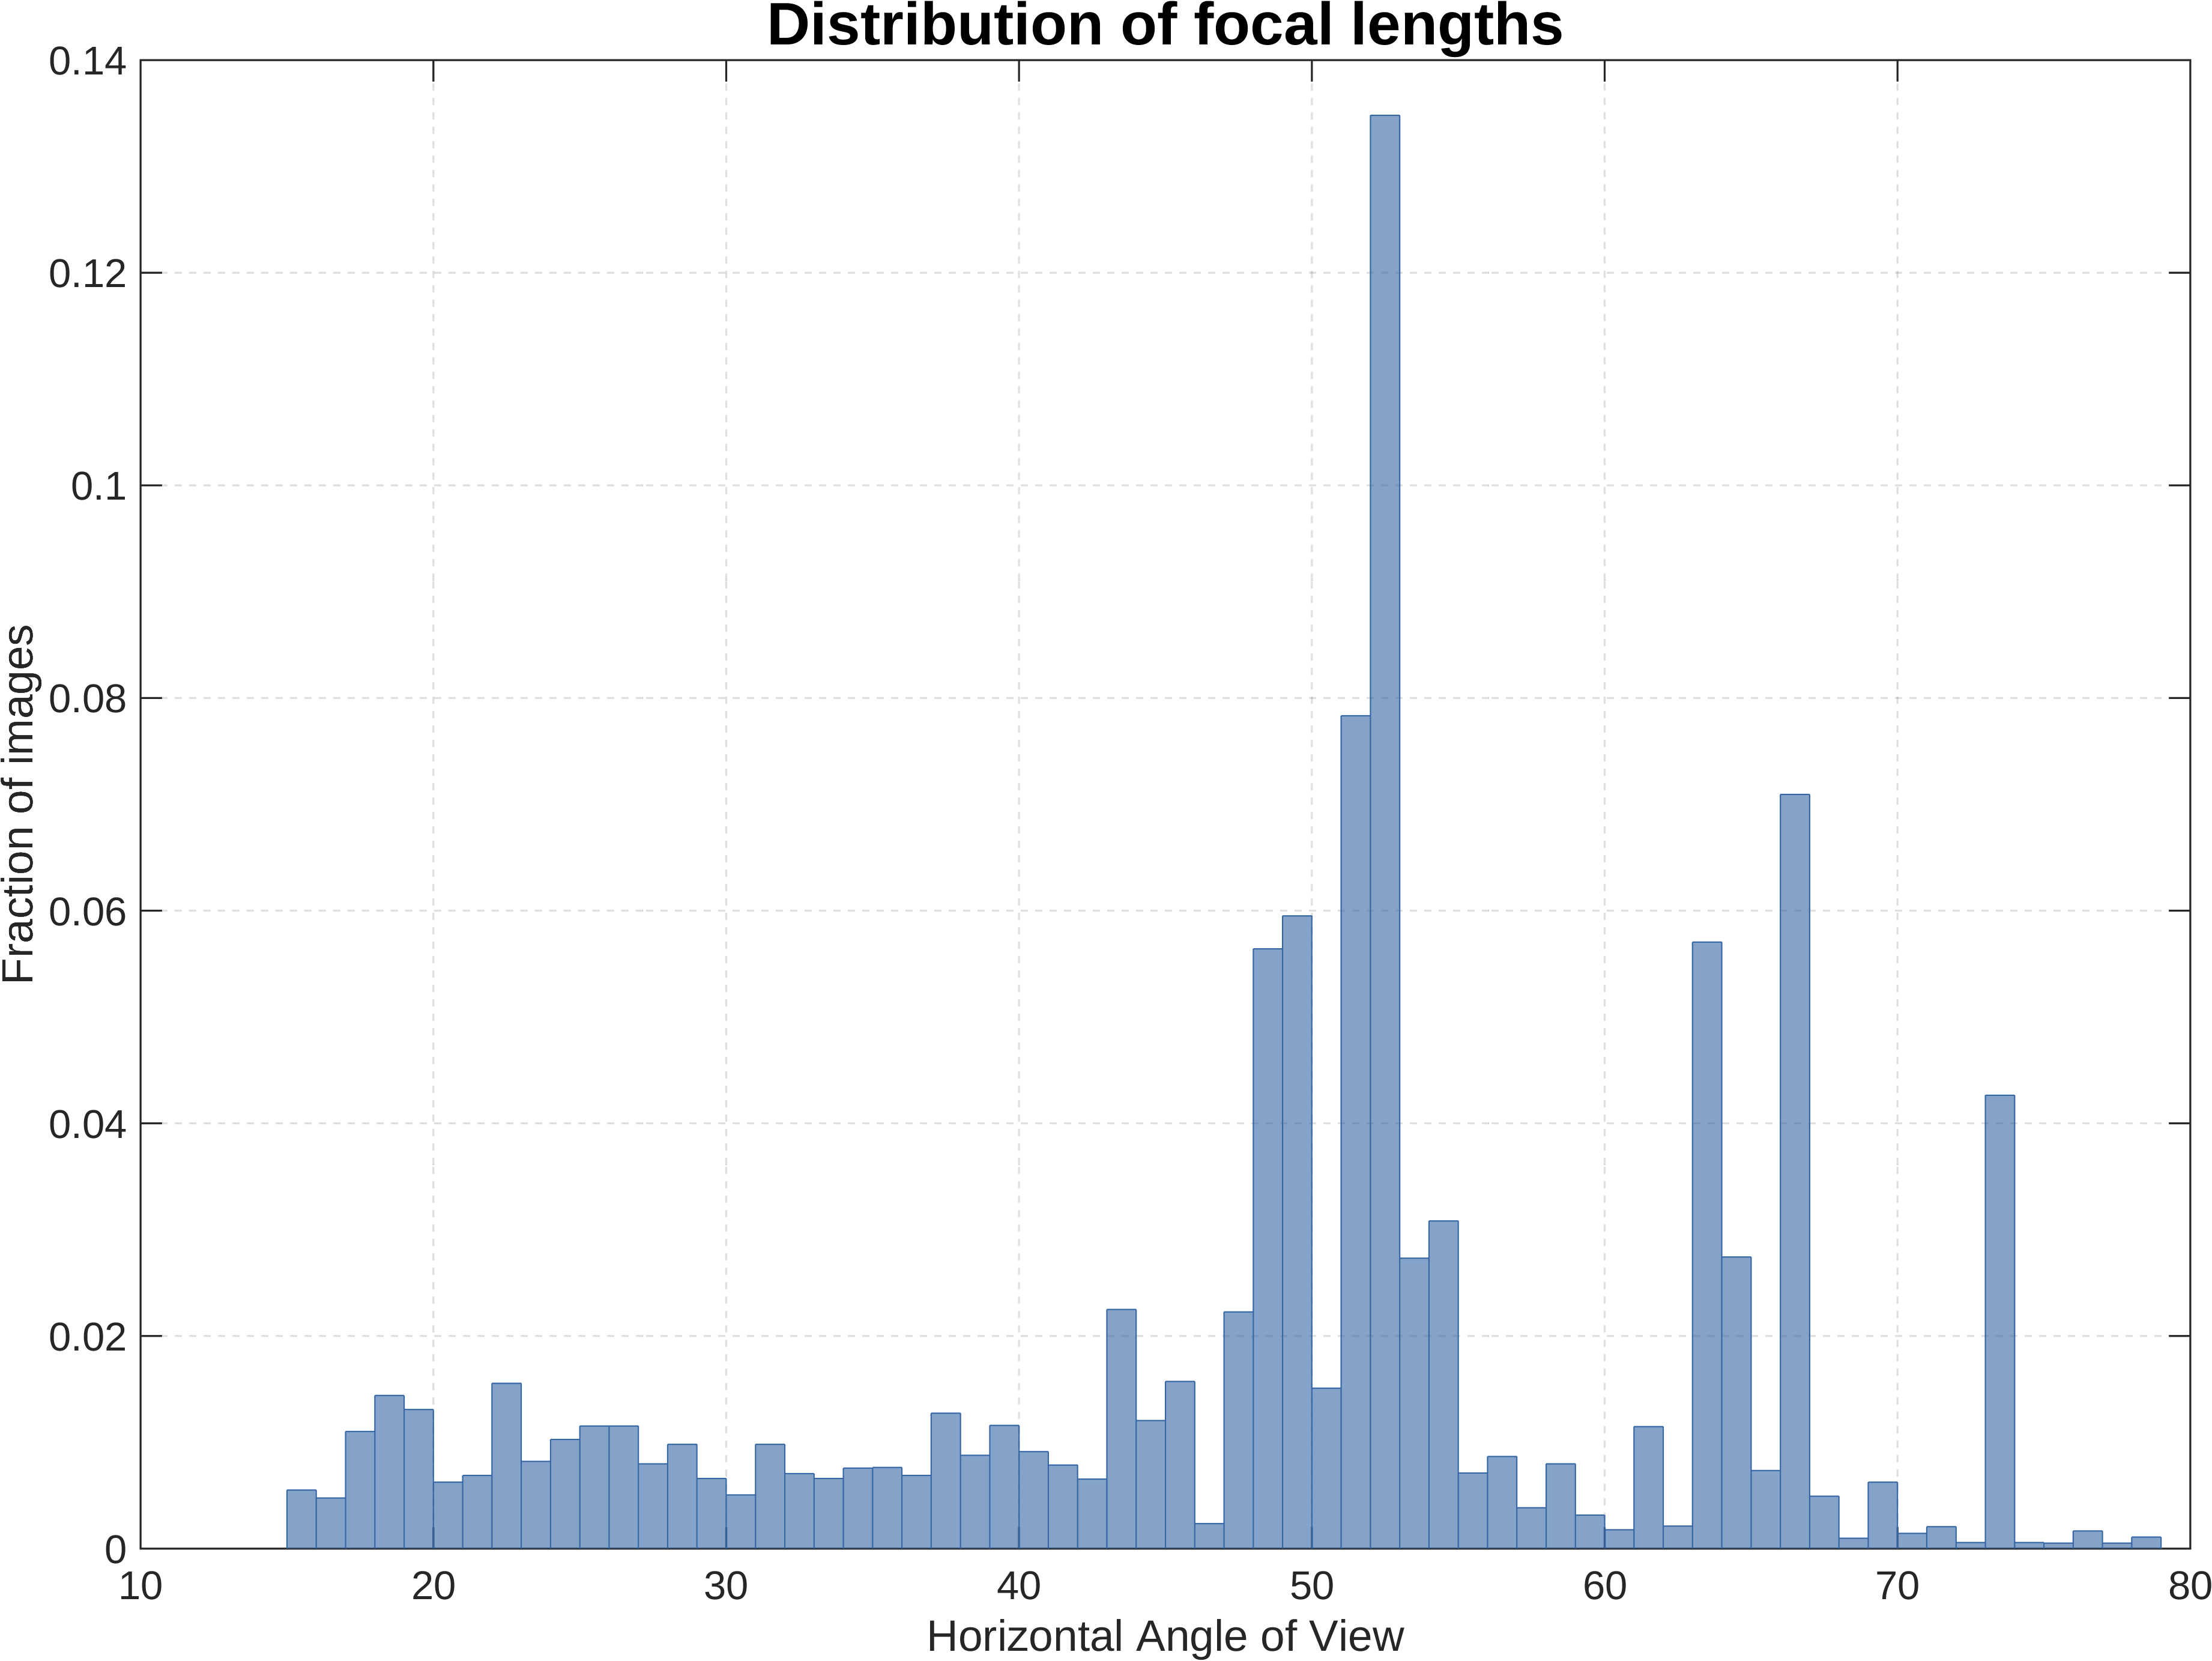
\includegraphics[width=0.95\linewidth]{figures/amodal/fov.png}
    \caption{\figlabel{fovDistr} Distribution of camera focal lengths in the Places dataset shown as horizontal angle of view. The peaks in the distribution correspond to canonical focal lengths in popular wide angle and telephoto lenses. It can be seen that the images cover the full spectrum from wide angle views of scenes (corresponding to the right end of the plot) to close-ups (left end of the histogram).}
  \end{minipage}
  \end{figure}

\paragraph{Results:} The results are shown in \tableref{focal_results} and suggest that focal length can indeed be predicted directly from images, at least approximately, and that pretraining on annotated scene class data makes a good match with this task. Our best model can predict correct focal length quite repeatably  among the top-three and top-five predictions. As baselines, we measure chance performance, and performance when picking the mode of the distribution on the training set -- the bin having most elements. The (unequal) distribution of the focal lengths can be seen in \figref{fovDistr}.


Note that our goal is not high precision of the type that is necessary for high-fidelity reconstruction; we aim for a coarse estimate of the focal length that can be robustly computed from natural images. Our results in this section are a first demonstration that this may be feasible.

\begin{table}
\centering
\resizebox{0.5\linewidth}{!}{
 \begin{tabular}{ l  c  c c}
\toprule
\textbf{Method} & \textbf{top-1} & \textbf{top-3} & \textbf{top-5} \\
\midrule
Chance & 90.0 & 70.0 & 50.0 \\
Mode Selection & 60.2 & 26.4 & 8.7 \\
\midrule
AlexNet-Imagenet & 57.1  & 18.8 & 3.9 \\
VGG-Deep16-Imagenet & 55.8 & 15.9 & 3.3 \\
PlacesNet-Places & \textbf{54.3} & \textbf{15.3} & \textbf{3.1} \\
\bottomrule
  \end{tabular}}
    \caption{\tablelabel{focal_results}Focal length misclassification rate (top-1, top-3 and top-5 predictions) of networks pretrained on object images from Imagenet and the Places dataset. Lower is better.}
\end{table}
%\newcommand{\gtViewWidth}{0.15}
\newcommand{\gtViewFormat}{pdf}
\begin{figure*}[htb!]
\includegraphics[width=\gtViewWidth\textwidth]{figures/categoryshapes/predictionVisualizationsVgg/aeroplane/42.\gtViewFormat} \hfill
\includegraphics[width=\gtViewWidth\textwidth]{figures/categoryshapes/predictionVisualizationsVgg/aeroplane/85.\gtViewFormat}
\includegraphics[width=\gtViewWidth\textwidth]{figures/categoryshapes/predictionVisualizationsVgg/aeroplane/125.\gtViewFormat} \hfill
\includegraphics[width=\gtViewWidth\textwidth]{figures/categoryshapes/predictionVisualizationsVgg/aeroplane/166.\gtViewFormat} \hfill
\includegraphics[width=\gtViewWidth\textwidth]{figures/categoryshapes/predictionVisualizationsVgg/aeroplane/207.\gtViewFormat}
\includegraphics[width=\gtViewWidth\textwidth]{figures/categoryshapes/predictionVisualizationsVgg/aeroplane/251.\gtViewFormat}

\includegraphics[width=\gtViewWidth\textwidth]{figures/categoryshapes/predictionVisualizationsVgg/bicycle/20.\gtViewFormat} \hfill
\includegraphics[width=\gtViewWidth\textwidth]{figures/categoryshapes/predictionVisualizationsVgg/bicycle/36.\gtViewFormat} \hfill
\includegraphics[width=\gtViewWidth\textwidth]{figures/categoryshapes/predictionVisualizationsVgg/bicycle/57.\gtViewFormat}
\includegraphics[width=\gtViewWidth\textwidth]{figures/categoryshapes/predictionVisualizationsVgg/bicycle/78.\gtViewFormat} \hfill
\includegraphics[width=\gtViewWidth\textwidth]{figures/categoryshapes/predictionVisualizationsVgg/bicycle/95.\gtViewFormat} \hfill
\includegraphics[width=\gtViewWidth\textwidth]{figures/categoryshapes/predictionVisualizationsVgg/bicycle/114.\gtViewFormat}

\includegraphics[width=\gtViewWidth\textwidth]{figures/categoryshapes/predictionVisualizationsVgg/bus/22.\gtViewFormat} \hfill
\includegraphics[width=\gtViewWidth\textwidth]{figures/categoryshapes/predictionVisualizationsVgg/bus/49.\gtViewFormat} \hfill
\includegraphics[width=\gtViewWidth\textwidth]{figures/categoryshapes/predictionVisualizationsVgg/bus/70.\gtViewFormat}
\includegraphics[width=\gtViewWidth\textwidth]{figures/categoryshapes/predictionVisualizationsVgg/bus/98.\gtViewFormat} \hfill
\includegraphics[width=\gtViewWidth\textwidth]{figures/categoryshapes/predictionVisualizationsVgg/bus/120.\gtViewFormat} \hfill
\includegraphics[width=\gtViewWidth\textwidth]{figures/categoryshapes/predictionVisualizationsVgg/bus/142.\gtViewFormat}

\includegraphics[width=\gtViewWidth\textwidth]{figures/categoryshapes/predictionVisualizationsVgg/car/49.\gtViewFormat} \hfill
\includegraphics[width=\gtViewWidth\textwidth]{figures/categoryshapes/predictionVisualizationsVgg/car/92.\gtViewFormat} \hfill
\includegraphics[width=\gtViewWidth\textwidth]{figures/categoryshapes/predictionVisualizationsVgg/car/137.\gtViewFormat}
\includegraphics[width=\gtViewWidth\textwidth]{figures/categoryshapes/predictionVisualizationsVgg/car/186.\gtViewFormat} \hfill
\includegraphics[width=\gtViewWidth\textwidth]{figures/categoryshapes/predictionVisualizationsVgg/car/232.\gtViewFormat} \hfill
\includegraphics[width=\gtViewWidth\textwidth]{figures/categoryshapes/predictionVisualizationsVgg/car/279.\gtViewFormat}

\includegraphics[width=\gtViewWidth\textwidth]{figures/categoryshapes/predictionVisualizationsVgg/chair/36.\gtViewFormat} \hfill
\includegraphics[width=\gtViewWidth\textwidth]{figures/categoryshapes/predictionVisualizationsVgg/chair/73.\gtViewFormat} \hfill
\includegraphics[width=\gtViewWidth\textwidth]{figures/categoryshapes/predictionVisualizationsVgg/chair/112.\gtViewFormat}
\includegraphics[width=\gtViewWidth\textwidth]{figures/categoryshapes/predictionVisualizationsVgg/chair/149.\gtViewFormat} \hfill
\includegraphics[width=\gtViewWidth\textwidth]{figures/categoryshapes/predictionVisualizationsVgg/chair/183.\gtViewFormat} \hfill
\includegraphics[width=\gtViewWidth\textwidth]{figures/categoryshapes/predictionVisualizationsVgg/chair/219.\gtViewFormat}

\includegraphics[width=\gtViewWidth\textwidth]{figures/categoryshapes/predictionVisualizationsVgg/motorbike/21.\gtViewFormat} \hfill
\includegraphics[width=\gtViewWidth\textwidth]{figures/categoryshapes/predictionVisualizationsVgg/motorbike/44.\gtViewFormat} \hfill
\includegraphics[width=\gtViewWidth\textwidth]{figures/categoryshapes/predictionVisualizationsVgg/motorbike/65.\gtViewFormat}
\includegraphics[width=\gtViewWidth\textwidth]{figures/categoryshapes/predictionVisualizationsVgg/motorbike/86.\gtViewFormat} \hfill
\includegraphics[width=\gtViewWidth\textwidth]{figures/categoryshapes/predictionVisualizationsVgg/motorbike/106.\gtViewFormat} \hfill
\includegraphics[width=\gtViewWidth\textwidth]{figures/categoryshapes/predictionVisualizationsVgg/motorbike/125.\gtViewFormat}

\caption{Viewpoint predictions for unoccluded groundtruth instances using our algorithm.  The columns show 15th, 30th, 45th, 60th, 75th and 90th percentile instances respectively in terms of the error. We visualize the predictions by rendering a 3D model using our predicted viewpoint.}
\label{figure:viewpointPreds}
\end{figure*}

\section{Experiments}
\seclabel{experiments}

We have presented several contributions towards the goal of object reconstruction from a single image -- \secref{modelLearning} proposed a method to learn deformable 3D models from an annotated image set, \secref{viewpoints} introduced a CNN based system to predict viewpoints and \secref{testing} put forward a framework for reconstructing objects from a single image. Our goal in the experiments was to empirically evaluate and qualitatively demonstrate the efficacy of each of these contributions.

We first  examine the quality and expressiveness of our learned 3D models by evaluating how well they matched the underlying 3D shapes of the training data (\secref{modelEval}). We also evaluate the accuracy of our viewpoint prediction system (\secref{vpExperiments}). We then study their sensitivity of obtained reconstructions when fit to images using noisy automatic segmentations and pose predictions (\secref{sensitivityAnalysis}) and finally present qualitative results for reconstructions from a single image (\secref{qualitativeRes}).


\subsection{Quality of Learned 3D Models}
\seclabel{modelEval}
The first question we address is whether the category-specific shape models we learn for each object class (\secref{modelLearning}) using an annotated image collection correctly explain the underlying 3D object shape for these annotated instances. Note that while it is not our final goal, this is itself a very challenging task - we have to obtain a dense 3D reconstruction for annotated images using just silhouettes and sparse keypoint correspondences. Recent work by Vicente \etal \cite{carvi14} addressed this task of `lifting' an annotated image collection to 3D and we compare the performance of our model learning stage against their approach. We also incorporate category-agnostic shape inflation  \cite{twarog2012playing} and intrinsic image \cite{Barron2012B} methods as baselines. The evaluation metrics, dataset and results are described below.

\vspace{3mm}
\noindent \textbf{Dataset.} We consider images from the challenging PASCAL VOC 2012 dataset~\cite{pascal-voc-2012} which contain objects from the 10 rigid object categories (as listed in Table \ref{tab:carvi_compare}). We use the publicly available ground truth class-specific keypoints~\cite{bourdevECCV10} and object segmentations~\cite{BharathICCV2011} to learn category-specific shape models for each class. We learn and fit our 3D models on the whole dataset (no train/test split), following the setup of Vicente \etal \cite{carvi14}.

Since ground truth 3D shapes are unavailable for PASCAL VOC and most other detection datasets, we evaluated the quality of our learned 3D models on the next best thing we managed to obtain: the PASCAL3D+ dataset~\cite{pascal3d} which has up to 10 3D CAD models for the rigid categories in PASCAL VOC. PASCAL3D+ provides between 4 different models for ``tvmonitor'' and ``train'' and 10 for ``car'' and ``chair''.
The subset of PASCAL we considered after filtering occluded instances, which we do not tackle in this paper, had between 70 images for ``sofa'' and 500 images for classes ``aeroplanes'' and ``cars''.

\vspace{3mm}
\noindent \textbf{Metrics.} We quantify the quality of our 3D models by comparing against the PASCAL 3D+ models using two metrics - 1) a mesh error metric computed as the Hausdorff distance between the ground truth and predicted mesh after translating both to the origin and normalizing by the diagonal of the tighest 3D bounding box of the ground truth mesh~\cite{aspert2002mesh} and 2) a depth map error to evaluate the quality of the reconstructed visible object surface, measured as the mean absolute distance between reconstructed and ground truth depth:
\begin{gather}
 Z\text{-MAE}(\hat{Z},Z^{*})=\frac{1}{n\cdot\gamma}\underset{\beta}{\text{min}}\underset{x,y}{\sum}|\hat{Z}_{x,y}-Z^*_{x,y}-\beta|
\end{gather}
where $\hat{Z}$ and $Z^*$ represent predicted and ground truth depth maps respectively. Analytically, $\beta$ can be computed as the median of $\hat{Z}-Z^*$ and $\gamma$ is a normalization factor to account for absolute object size for which we use the bounding box diagonal. Note that our depth map error is translation and scale invariant.

\vspace{3mm}
\noindent \textbf{Results.}
We report the performance of our model learning approach in Table \ref{tab:carvi_compare}. Here, `SIRFS' denotes a state-of-the art intrinsic image decomposition method and `Puffball'l\cite{twarog2012playing} denotes a shape-inflation method for reconstruction.  `Carvi' denotes the recent method by Vicente \etal \cite{carvi14} which is specifically designed for the task of reconstructing an annotated image collection as their visual hull based reconstruction technique makes strong assumptions regarding the accuracy of the object mask and predicted viewpoint.

We observe that category-agnostic methods -- Puffball\cite{twarog2012playing} and SIRFS\cite{barronPAMI13, Barron2012B} -- consistently perform worse on the benchmark by themselves as they use generic priors to reconstruct each image individually and cannot reason over the image collection jointly. Our model learning performs comparably to the specialized approach of Vicente \etal -- we demonstrate competitive, if not better, performance on both benchmarks with our models showing greater robustnes to perspective foreshortening effects on ``trains'' and ``buses''.  Certain classes like ``boat'' and ``sofa'' are especially hard because of large intra-class variance and data sparsity respectively.

\subsection{Accuracy of Viewpoint Estimation}
%\section{Experiments : Viewpoint Prediction}
\seclabel{vpExperiments}

\renewcommand{\arraystretch}{1.4}
\setlength{\tabcolsep}{6pt}
\begin{table*}
\centering
\resizebox{1.0\linewidth}{!}{
\begin{tabular}{lcccccccccccc|c}
\toprule
 & \textbf{\footnotesize{}aero} & \textbf{\footnotesize{}bike} & \textbf{\footnotesize{}boat} & \textbf{\footnotesize{}bottle} & \textbf{\footnotesize{}bus} & \textbf{\footnotesize{}car} & \textbf{\footnotesize{}chair} & \textbf{\footnotesize{}table} & \textbf{\footnotesize{}mbike} & \textbf{\footnotesize{}sofa} & \textbf{\footnotesize{}train} & \textbf{\footnotesize{}tv} & \textbf{\footnotesize{}mean}\tabularnewline
\midrule
{\footnotesize{}$Acc_{\frac{\pi}{6}}$ (Pool5-TNet)} & {\footnotesize{}0.27} & {\footnotesize{}0.18} & {\footnotesize{}0.36} & {\footnotesize{}0.81} & {\footnotesize{}0.71} & {\footnotesize{}0.36} & {\footnotesize{}0.52} & {\footnotesize{}0.52} & {\footnotesize{}0.38} & {\footnotesize{}0.67} & {\footnotesize{}0.70} & {\footnotesize{}0.71} & {\footnotesize{}0.52}\tabularnewline
{\footnotesize{}$Acc_{\frac{\pi}{6}}$(fc7-TNet)} & {\footnotesize{}0.50} & {\footnotesize{}0.44} & {\footnotesize{}0.39} & {\footnotesize{}0.88} & {\footnotesize{}0.81} & {\footnotesize{}0.70} & {\footnotesize{}0.39} & {\footnotesize{}0.38} & {\footnotesize{}0.48} & {\footnotesize{}0.44} & {\footnotesize{}0.78} & {\footnotesize{}0.65} & {\footnotesize{}0.57}\tabularnewline
{\footnotesize{}$Acc_{\frac{\pi}{6}}$(ours-TNet)} & {\footnotesize{}0.78} & {\footnotesize{}0.74} & {\footnotesize{}0.49} & \textbf{\footnotesize{}0.93} & {\footnotesize{}0.94} & \textbf{\footnotesize{}0.90} & {\footnotesize{}0.65} & \textbf{\footnotesize{}0.67} & {\footnotesize{}0.83} & {\footnotesize{}0.67} & {\footnotesize{}0.79} & {\footnotesize{}0.76} & {\footnotesize{}0.76}\tabularnewline
{\footnotesize{}$Acc_{\frac{\pi}{6}}$(ours-ONet)} & \textbf{\footnotesize{}0.81} & \textbf{\footnotesize{}0.77} & \textbf{\footnotesize{}0.59} & \textbf{\footnotesize{}0.93} & \textbf{\footnotesize{}0.98} & {\footnotesize{}0.89} & \textbf{\footnotesize{}0.80} & \textbf{\footnotesize{}0}{\footnotesize{}.62} & \textbf{\footnotesize{}0.88} & \textbf{\footnotesize{}0.82} & \textbf{\footnotesize{}0.80} & \textbf{\footnotesize{}0.80} & \textbf{\footnotesize{}0.81}\tabularnewline
\midrule
{\footnotesize{}$MedErr$ (Pool5-TNet)} & {\footnotesize{}42.6} & {\footnotesize{}52.3} & {\footnotesize{}46.3} & {\footnotesize{}18.5} & {\footnotesize{}17.5} & {\footnotesize{}45.6} & {\footnotesize{}28.6} & {\footnotesize{}27.7} & {\footnotesize{}37.0} & {\footnotesize{}25.9} & {\footnotesize{}20.6} & {\footnotesize{}21.5} & {\footnotesize{}32.0}\tabularnewline
{\footnotesize{}$MedErr$(fc7-TNet)} & {\footnotesize{}29.8} & {\footnotesize{}40.3} & {\footnotesize{}49.5} & {\footnotesize{}13.5} & {\footnotesize{}7.6} & {\footnotesize{}13.6} & {\footnotesize{}45.5} & {\footnotesize{}38.7} & {\footnotesize{}31.4} & {\footnotesize{}38.5} & {\footnotesize{}9.9} & {\footnotesize{}22.6} & {\footnotesize{}28.4}\tabularnewline
{\footnotesize{}$MedErr$(ours-TNet)} & {\footnotesize{}14.7} & {\footnotesize{}18.6} & {\footnotesize{}31.2} & {\footnotesize{}13.5} & {\footnotesize{}6.3} & \textbf{\footnotesize{}8.8} & {\footnotesize{}17.7} & {\footnotesize{}17.4} & {\footnotesize{}17.6} & {\footnotesize{}15.1} & {\footnotesize{}8.9} & {\footnotesize{}17.8} & {\footnotesize{}15.6}\tabularnewline
{\footnotesize{}$MedErr$(ours-ONet)} & \textbf{\footnotesize{}13.8} & \textbf{\footnotesize{}17.7} & \textbf{\footnotesize{}21.3} & \textbf{\footnotesize{}12.9} & \textbf{\footnotesize{}5.8} & {\footnotesize{}9.1} & \textbf{\footnotesize{}14.8} & \textbf{\footnotesize{}15.2} & \textbf{\footnotesize{}14.7} & \textbf{\footnotesize{}13.7} & \textbf{\footnotesize{}8.7} & \textbf{\footnotesize{}15.4} & \textbf{\footnotesize{}13.6}\tabularnewline
\bottomrule
\end{tabular}}
\caption{Viewpoint Estimation with Ground Truth box}
\label{table:poseGtEval}
\end{table*}

An important component of the proposed reconstruction framework is the viewpoint estimation system \secref{viewpoints} which allows us to fit learned models to objects in new images. We evaluate this component under two settings -- viewpoint prediction accuracy when the object localization is known and a detection setting with unkown localization. We observe that our proposed approach significantly improves the state-of-the-art for viewpoint estimation in both these settings.

\vspace{3mm}
\noindent \textbf{Dataset.}
Xiang \etal \cite{pascal3d} provide annotations for $(\phi,\varphi,\psi)$ corresponding to all the instances in the PASCAL VOC 2012 detection train, validation set as well as for ImageNet images. We use the PASCAL train set and the ImageNet annotations to train the CNN described in \secref{viewpoints} and use the PASCAL VOC 2012 validation set annotations to evaluate our performance. 

\vspace{3mm}
\noindent \textbf{Viewpoint Estimation with Ground Truth box.}
To analyze the performance of our viewpoint estimation method independent of factors like mis-localization, we first tackle the task of estimating the viewpoint of an object with known bounds. Let $\Delta(R_1,R_2) = \frac{ \| log(R_1^TR_2)\|_F}{\sqrt{2}}$ denote the geodesic distance function over the manifold of rotation matrices. $\Delta(R_{gt},R_{pred})$ captures the difference between ground truth viewpoint $R_{gt}$ and predicted viewpoint $R_{pred}$. We use two complementary metrics for evaluation -
\begin{itemize}
\item \textbf{Median Error :} The common confusions for the task of viewpoint estimation often are predictions which are far apart (eg. left facing vs right facing car) and the median error ($MedErr$) is a widely use metric that is robust to these if a significant fraction of the estimates are accurate.
\item \textbf{Accuracy at $\theta$ :} A small median error does not necessarily imply accurate estimates for all instances, a complementary performance measure is the fraction of instances whose predicted viewpoint is within a fixed threshold of the target viewpoint. We denote this metric by $Acc_{\theta}$ where $\theta$ is the threshold. We use $\theta = \frac{\pi}{6}$.
\end{itemize}
Recently, Ghodrati \etal \cite{ghodrati14viewpoint} achieved results comparable to state-of-the art by using a linear classifier over layer 5 features of TNet. We denote this method as 'Pool5-TNet' and implement it as a baseline. To study the effect of end-to-end training of the CNN architecture, we use a linear classifier on top of the fc7 layer of TNet as another baseline (denoted as 'fc7-TNet' ). With the aim of  analyzing viewpoint estimation independently, the evaluations were restricted only to objects marked as non-occluded and non-truncated. The performance of our method and comparisons to the baseline are shown in Table \ref{table:poseGtEval}. The results clearly demonstrate that end-to-end training improves results and that our method with the TNet architecture performs significantly better than the 'Pool5-TNet' method used in \cite{ghodrati14viewpoint}. We also observe a significant improvement by using the ONet architecture and only use this architecture for further experiments/analysis. In Figure \ref{figure:viewpointPreds}, we show our predictions sorted in terms of the error and  it can be seen that the predictions for most categories are reliable even at the 90th percentile.

\renewcommand{\arraystretch}{1.4}
\setlength{\tabcolsep}{6pt}
\begin{table}[htb!]
\centering
\resizebox{1.0\linewidth}{!}{
\begin{tabular}{lcccccc}
\toprule
 &  \multicolumn{4}{c}{\footnotesize{}$AVP$} &  {\footnotesize{}$AVP_{\frac{\pi}{6}}$} & {\footnotesize{}$ARP_{\frac{\pi}{6}}$} \tabularnewline
\midrule
\textbf{\footnotesize{}Number of bins} & \textbf{\footnotesize{}4 } & \textbf{\footnotesize{}8} & \textbf{\footnotesize{}16} & \textbf{\footnotesize{}24} & \textbf{\footnotesize{}-} & \textbf{\footnotesize{}-}\tabularnewline
\midrule
\textbf{\footnotesize{}Xiang \etal \cite{pascal3d}} & {\footnotesize{}19.5} & {\footnotesize{}18.7} & {\footnotesize{}15.6} & {\footnotesize{}12.1} & {\footnotesize{}-} & {\footnotesize{}-}\tabularnewline
\textbf{\footnotesize{}Pepik \etal \cite{pepik12dpm}} & {\footnotesize{}23.8} & {\footnotesize{}21.5} & {\footnotesize{}17.3} & {\footnotesize{}13.6} & {\footnotesize{}-} & {\footnotesize{}-}\tabularnewline
\textbf{\footnotesize{}Ghodrati \etal \cite{ghodrati14viewpoint}} & {\footnotesize{}24.1} & {\footnotesize{}22.3} & {\footnotesize{}17.3} & {\footnotesize{}13.7} & {\footnotesize{}-} & {\footnotesize{}-}\tabularnewline
\textbf{\footnotesize{}ours} & \textbf{\footnotesize{}49.1} & \textbf{\footnotesize{}44.5} & \textbf{\footnotesize{}36.0} & \textbf{\footnotesize{}31.1} & {\footnotesize{}50.7} & {\footnotesize{}46.5}\tabularnewline
\bottomrule
\end{tabular}}

\caption{Mean performance of our approach for various metrics. The detailed results for  individual classes can be found at the PASCAL3D leaderboard (\url{http://cvgl.stanford.edu/projects/pascal3d.html}).}
\label{table:poseDetEval}
\end{table}

\vspace{3mm}
\noindent \textbf{Viewpoint Estimation with Detection.}
Xiang \etal \cite{pascal3d} introduced the $AVP$ metric to measure advances in the task of viewpoint estimation in the setting where localizations are not known a priori. The metric is similar to the $AP$ criterion used for PASCAL VOC detection except that each detection candidate has an associated viewpoint and the detection is labeled correct if it has a correct predicted viewpoint bin as well as a correct localization (bounding box IoU $>$ 0.5). Xiang \etal \cite{pascal3d} also compared to Pepik \etal \cite{pepik12dpm} on the AVP metric using various viewpoint bin sizes and Ghodrati \etal \cite{ghodrati14viewpoint} also showed comparable results on the metric. To evaluate our method, we obtain detections from RCNN \cite{rcnn} using MCG \cite{mcg2014} object proposals and augment them with a pose predicted using the corresponding detection's bounding box.

We note that there are two issues with the $AVP$ metric - it only evaluates the prediction for the azimuth ($\phi$) angle and discretizes viewpoint instead of treating it continuously. Therefore, we also introduce two additional evaluation metrics which follow the IoU $>$ 0.5 criteria for localization but modify the criteria for assigning a viewpoint prediction to be correct as follows -
\begin{itemize}
\item $AVP_{\theta}$ : $\delta(\phi_{gt},\phi_{pred})<\theta$
\item $ARP_{\theta}$ :  $\Delta(R_{gt},R_{pred})<\theta$
\end{itemize}
Note that $ARP_{\theta}$ requires the prediction of all euler angles instead of just $\phi$ and therefore, is a stricter metric.

The performance of our CNN based approach for viewpoint prediction in the detection setting is shown in Table \ref{table:poseDetEval} and it can be seen that we significantly outperform the state-of-the-art methods across all categories. While it is not possible to compare our pose estimation performance independent of detection with DPM based methods like \cite{pascal3d,pepik12dpm}, an indirect comparison results from the analysis using ground truth boxes where we demonstrate that our pose estimation approach is an improvement over \cite{ghodrati14viewpoint} which in turn performs similar to \cite{pascal3d,pepik12dpm} while using similar detectors.

% \begin{table}[htb!]
        \centering
        \begin{tabular}{lcc}
\toprule
\textbf{\footnotesize{}Setting} & \textbf{\footnotesize{}Mean Error} & \textbf{\footnotesize{}Mean Accuracy}\tabularnewline
\midrule
{\footnotesize{}Default} & {\footnotesize{}13.5} & {\footnotesize{}0.81}\tabularnewline
{\footnotesize{}Small Objects} & {\footnotesize{}15.1} & {\footnotesize{}0.75}\tabularnewline
{\footnotesize{}Large Objects} & {\footnotesize{}12.7} & {\footnotesize{}0.87}\tabularnewline
{\footnotesize{}Occluded Objects} & {\footnotesize{}19.9} & {\footnotesize{}0.65}\tabularnewline
\bottomrule
\end{tabular}
        \caption{Object characteristics vs viewpoint prediction error}
        \label{table:vpObjectModes}
    \end{table}

 \begin{table}[htb!]
 \centering
\begin{tabular}{cc}
\toprule
\textbf{\footnotesize{}Setting} & \textbf{\footnotesize{}Accuracy}\tabularnewline
\midrule
{\footnotesize{}Error$<\frac{\pi}{9}$} & {\footnotesize{}83.7}\tabularnewline
{\footnotesize{}$\frac{\pi}{9}<$Error $<\frac{2\pi}{9}$} & {\footnotesize{}5.7}\tabularnewline
{\footnotesize{}Error$>\frac{\pi}{9}$ \& Error($\pi-flip$)$<\frac{\pi}{9}$} & {\footnotesize{}5.8}\tabularnewline
{\footnotesize{}Error$>\frac{\pi}{9}$ \& Error($z-ref$)$<\frac{\pi}{9}$} & {\footnotesize{}6.5}\tabularnewline
{\footnotesize{}Other} & {\footnotesize{}2.9}\tabularnewline
\bottomrule
\end{tabular}
		\caption{Analysis of error modes for viewpoint prediction}
		\label{table:vpErrorModes}        
 \end{table}


An understanding of failure cases and effect of object characteristics on performance can often suggest insights for future directions. Hoeim \etal \cite{hoiem2012diagnosing} suggested some excellent diagnostics for object detection systems and we adapt those  for the task of pose estimation. We evaluate our system's output for both the task of viewpoint prediction as well as keypoint prediction but restrict our analysis to the setting with known bounding boxes - this enables us to analyze our pose estimation method independent of the detection system. We denote as 'large objects' the top third of instances and by 'small objects' the bottom third of instances. The label 'occluded' describes all the objects marked as truncated or occluded according to the PASCAL VOC annotations. We summarize our observations below.

\paragraph{Object Characteristics : } Table \ref{table:vpObjectModes} shows the effect of object characteristics by reporting the mean across the classes of the median viewpoint error and accuracy. We can see that the method performs worse for occluded objects. There is also a significant difference between the performance for small and large objects - while such error trends are acceptable in the robotic setting where ambiguity for the farther objects is tolerable, one may need to capture more context to perform well without higher resolution input.

\paragraph{Error Modes: }
Since it is difficult to characterize error modes for generic rotations, we restrict the analysis to only the predicted azimuth. Assuming the image plane to be XY, we denote by $Z-ref$ the pose for the instance reflected along the XY plane and by $\pi-flip$ a rotation of $\pi$ along the $Z$ axis. Table \ref{table:vpErrorModes} reports the percentage of instances whose predicted pose corresponds to various modes. We observe that these error modes are equally common  and that only about $3\%$ of the errors are not explained by these.

Note that we exclude 'diningtable' and 'bottle' categories from the above analysis due to small number of unoccluded instances and insignificant variations respectively.

\subsection{Sensitivity Analysis for Recognition based Reconstruction} 
\seclabel{sensitivityAnalysis}
\renewcommand{\arraystretch}{1.4} 
\setlength{\tabcolsep}{8pt}
\begin{table*}
\centering
\footnotesize
\resizebox{1.0\linewidth}{!}{
\begin{tabular}{cccccccccccc|c}
\toprule 
	& 	& \textbf{aero}	& \textbf{bike}	& \textbf{boat}	& \textbf{bus}	& \textbf{car}	& \textbf{chair}	& \textbf{mbike}	& \textbf{sofa}	& \textbf{train}	& \textbf{tv}	& \textbf{mean}
\\
\midrule

\multirow{3}{*}{\textbf{Mesh}} 	& KP+Mask	& 1.77 & 1.85 & 3.68 & 1.90 & 1.80 & 2.26 & 1.83 & 6.86 & 2.69 & 3.40 & 2.80 \\
& KP+SDS	& 1.75 & 1.89 & 3.71 & 1.87 & 1.75 & 2.27 & 1.84 & 6.56 & 2.76 & 3.39 & 2.78 \\
& PP+SDS	& 1.84 & 2.02 & 4.59 & 1.86 & 1.88 & 2.41 & 2.01 & 7.30 & 2.74 & 3.27 & 2.99 \\
& Puff~\cite{twarog2012playing} & 3.31 & 2.49 & 2.95 & 3.40 & 2.87 & 3.09 & 2.65 & 2.73 & 3.91 & 3.33 & 3.07 \\
\midrule
\multirow{3}{*}{\textbf{Depth}} 	& KP+Mask	& 9.83 & 9.95 & 21.07 & 12.80 & 10.07 & 9.10 & 9.98 & 29.39 & 25.70 & 9.85 & 14.77 \\
& KP+SDS	& 9.95 & 10.35 & 20.11 & 13.06 & 10.49 & 9.24 & 10.61 & 27.94 & 26.13 & 10.10 & 14.80 \\
& PP+SDS	& 11.42 & 11.25 & 21.93 & 22.04 & 13.69 & 10.27 & 11.71 & 26.76 & 34.92 & 9.88 & 17.39 \\
& SIRFS~\cite{barronPAMI13} & 13.58 & 14.48 & 19.64 & 30.14 & 22.60 & 20.12 & 16.81 & 21.54 & 41.40 & 23.67 & 22.40 \\
\bottomrule
\end{tabular}}
\caption{Ablation study for our method assuming/relaxing various annotations at test time on objects in PASCAL VOC. As can be seen, our method degrades gracefully with relaxed annotations. Note that these experiments are in a train/test setting and numbers will differ from Table \ref{tab:carvi_compare}. Please see text for more details.}
\label{tab:ablation}
\end{table*}

\begin{figure*}[htbp!]
  \includegraphics[width = \textwidth]{figures/categoryshapes/resultfig1.pdf}
  \caption{Fully automatic reconstructions on detected instances (0.5 IoU with ground truth) using our models on rigid categories in PASCAL VOC. We show our instance segmentation input, the inferred shape overlaid on the image, a 2.5D depth map (after the bottom-up refinement stage), the mesh in the image viewpoint and two other views. It can be seen that our method produces plausible reconstructions which is a remarkable achievement given just a single image and noisy instance segmentations. Color encodes depth in the image coordinate frame (blue is closer). More results can be found at \url{https://goo.gl/MgVQzZ}.}
  \label{fig:recons}
\end{figure*}

Our primary goal is to reconstruct objects in an image automatically. Towards this goal, we study the performance of our system when relaxing the availability of various  expensive annotations of the form of keypoint correspondences or instance segmentations. 

\vspace{3mm}
\noindent \textbf{Dataset and Metrics.}
The reconstruction error metrics for measuring mesh and depth error are the same as described previously (\secref{modelEval}). The segmentation, keypoint annotations for learning and the mesh annotations for evaluation are also similarly obtained. However, for the sensitivity analysis, we introduce a train/test split since the recognition components used for instance segmentation and viewpoint estimation are trained on the PASCAL VOC train set. We therefore train our category-shape models  on only the subset of the data corresponding to PASCAL VOC train set. We then reconstruct the held out objects in the PASCAL validation set and report performance for these test objects.

\vspace{3mm}
\noindent \textbf{Results.}
In order to analyze sensitivity of our models to noisy inputs we reconstructed held-out test instances using our models given just ground truth bounding boxes. We compare various versions of our method using ground truth(Mask)/imperfect segmentations(SDS) and keypoints(KP)/our pose predictor(PP) for viewpoint estimation respectively. For pose prediction, we use the CNN-based system described in \secref{viewpoints}. To obtain an approximate segmentation from the bounding box, we use the refinement stage of the state-of-the-art joint detection and segmentation system proposed in \cite{BharathECCV2014}. 

Table \ref{tab:ablation} shows that our results degrade gracefully from the fully annotated to the fully automatic setting. Our method is robust to some mis-segmentation owing to our shape model that prevents shapes from bending unnaturally to explain noisy silhouettes. Our reconstructions degrade slightly with imperfect pose initializations even though our projection parameter optimization deals with it to some extent. With predicted poses, we observe that sometimes even when our reconstructions look plausible, the errors can be high as the metrics are sensitive to bad alignment. The data sparsity issue is especially visible in the case of sofas where in a train/test setting in Table \ref{tab:ablation} the numbers drop significantly with less training data (only 34 instances). Note we do not evaluate our bottom-up component as the PASCAL 3D+ meshes provided do not share the same high frequency shape details as the instance.

\subsection{Fully Automatic Reconstruction}
\seclabel{qualitativeRes}
We qualitatively demonstrate reconstructions on automatically detected and segmented instances with 0.5 IoU overlap with the ground truth in whole images in PASCAL VOC using \cite{BharathECCV2014} in Figure \ref{fig:recons}. We can see that our method is able to deal with some degree of mis-segmentation. Some of our major failure modes include not being able to capture the correct scale and pose of the object and thus badly fitting to the silhouette in some cases.


%\input{applications}
\section{Discussion}
We proposed what may be the first approach to perform fully automatic object reconstruction from a single image on a large and realistic dataset. Critically, our deformable 3D shape model can be bootstrapped from easily acquired ground-truth 2D annotations thereby bypassing the need for a-priori manual mesh design or 3D scanning and making it possible for convenient use of these types of models on large real-world datasets (e.g. PASCAL VOC). We report an extensive evaluation of the quality of the learned 3D models on a 3D benchmarking dataset for PASCAL VOC~\cite{pascal3d} showing competitive results with models that specialize in shape reconstruction using ground truth annotations as inputs while demonstrating that our method is equally capable in the wild, on top of automatic object detectors.

Much research lies ahead, both in terms of improving the quality and the robustness of reconstruction at test time (both bottom-up and top-down components), developing benchmarks for joint recognition and reconstruction and relaxing the need for annotations during training: all of these constitute interesting and important directions for future work. More expressive non-linear shape models \cite{wu20143d} may prove helpful (we present an instance in Chapter \ref{chapter:LSM} with LSMs), as well as a tighter integration between segmentation and reconstruction.

%For now, our models are likely to be useful for 3D-oriented recognition approaches \cite{SavareseF07,zia2013detailed,fidler20123d}.
%\todo{Remove all supplementary references ?}
%For now, our models are likely to be useful for 3D-oriented recognition approaches \cite{zia2013detailed,fidler20123d}.

%The existence of strong dependencies between object reconstruction, recognition and segmentation in human vision has been well demonstrated (e.g. \cite{nandakumar2011little}) and we hope our work will contribute exploiting similar interactions in the computational setting. 

%  and found this to lead to more accurate reconstruction compared to using either process in isolation. 
This dissertation is a product of the love and guidance of a great many people who contributions to this perhaps outweigh any of mine. First and foremost, I would like to thank my advisor, Jitendra Malik, for teaching me how to pursue impactful research, the numerous history lessons and having my back whenever I faltered. I wouldn't trade advisors for anything in this world. Thank you Alyosha Efros for (re)-introducing me to the treasure that is Berkeley and guiding me through testing times both as a mentor and an academic ``brother''. Thanks to my quals and thesis committee members Bruno Olshausen and Pieter Abbeel for valuable feedback on my research.

I have had the great fortune to be surrounded by some of the smartest and most empathetic people during my time at Berkeley. Thanks to my co-authors - Shubham Tulsiani who taught me great many things including the art of asking the right questions, Jo\~ao Carreira for his artful writing and Christian H\"ane for deepening my knowledge in 3D vision. Thanks to everyone in Malik and Efros groups: Saurabh, Bharath, Pablo, Jon Barron, Georgia, Pulkit, Panna, Ross, Deepak, Tinghui, Jun-Yan, Richard, Shiry, David, Evan, Judy and others, for all the discussions in the lab. My ideas and opinions have been greatly shaped by the discussions and I have learned immensely from them. I would also like to thank Angie Abbatecola for never letting the Berkeley bureaucracy bog me down and always being there to help.

My experience during grad school has been made ever so enjoyable by my amazing support group of friends. Thank you Sakshi, Somil, Tejas, Mobin, Smeet and Shiva for being there when the going got tough. Thanks to my group of friends away from home (Berkeley) - Partha, Sanjay and Pramit, for keeping me going. Thanks Varsha for always believing in me and helping me become a better human being over these years. Finally, I would like to thank the three most important people in my life: my father, mother and brother (Amlan). Thank you for giving me the freedom to pursue my dreams, teaching me the immense value of helping others and never letting me feel alone 8000 miles away.

{\small
\bibliographystyle{ieee}
\bibliography{referencesClean}
}

\end{document}
